\chapter{Gráficos en 3D}

Con \textbf{MATLAB} Se pueden realizar curvas en el espacio y superficies 3D. Un ejemplo de curvas en el espacio son las curvas de nivel, las cuales en realidad son representaciones bi-dimensionales que tras su posterior interpretación nos conducen al entorno espacial.

Algunos tipos de gráficos 3D que se pueden realizar con \textbf{MATLAB}:
\begin{center}
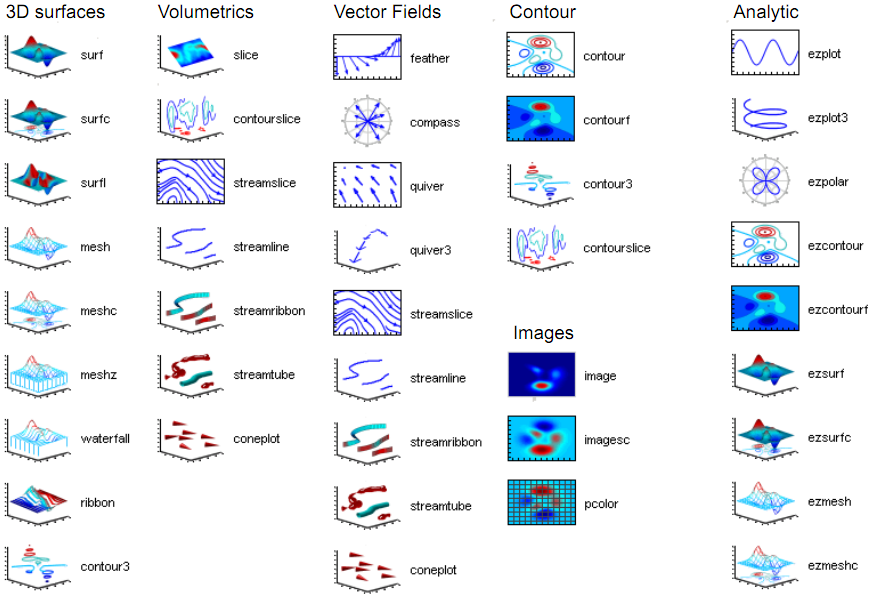
\includegraphics[width=450pt]{./Imagenes/graficos3d.png}
\end{center}

\section{Curvas en el espacio}

Existe una conexión muy estrecha entre las funciones vectoriales continuas de una variable con 
las curvas.

Una función vectorial \textbf{r} definida sobre un intervalo $I=[a,b]$, es una correspondencia entre los puntos de $I$ con los vectores del espacio, mediante $r(t)=(x(t),y(t),z(t)); t \in I$.

La función vectorial \textbf{r} es continua en \textbf{t=c} si y solo si sus funciones componentes \textbf{x,y,z} son continuas en \textbf{t=c}.

Dado un punto \textbf{P(x;y;z)} en el espacio, el vector $r(t)=x_{i}+y_{j}+z_{k}$ es el vector posición del punto \textbf{P}. A cada punto le corresponde un único vector posición y viceversa. 

\section{El comando plot3}

Este comando se utiliza para representar curvas en el espacio. Su funcionamiento y manejo es similar al del comando \textbf{plot}. La sintaxis del comando es:

\begin{lstlisting}[language=Matlab]
>> plot3(x,y,z,opciones)
\end{lstlisting}

En el campo opciones, se utilizan las mismas que vimos anteriormente para el comando \textbf{plot}.

El ejemplo que veremos a continuación corresponde a una curva alabeada $(x(t), y(t), z(t)), t \in [t_{0}, t_{f} ]$, con la orden $plot3(x,y,z)$:

\begin{lstlisting}[language=Matlab]
>> t=linspace(0,50,500);
>> x=t.*cos(t); y=t.*sin(t); z=t;
>> plot3(x,y,z)
>> xlabel('x(t)'); ylabel('y(t)'); zlabel('z(t)');
>> grid on; title('Curva con plot3');
\end{lstlisting}
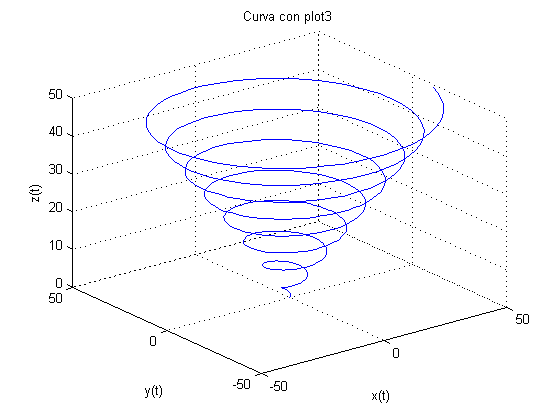
\includegraphics[width=300pt]{./Imagenes/3d1.png}


\section{El comando surf}

El comando \textbf{surf} se utiliza para representar superficies en el espacio. Esencialmente sirve para representar funciones de dos variables en el espacio. La sintaxis de este comando es:

\begin{lstlisting}[language=Matlab]
>> surf(x,y,z)
\end{lstlisting}

donde \textbf{X} e \textbf{Y} especifican una malla en el plano y \textbf{Z} la altura correspondiente. El color que se le da a cada punto esta asignado por defecto según la altura del eje Z.

Lo que debemos hacer ahora es construir una malla. Para esto utilizaremos el comando \textbf{meshgrid}. De esta forma podremos representar una superficie $ z = f(x,y) $ en un dominio rectangular, utilizando puntos de coordenadas $ x = (x_{1},\ldots, x_{n}) $ e $ y = (y_{1},\ldots, y_{n}) $. Con estos puntos podremos generar una malla donde los nuevos puntos sean $ x_{i},y_{j} $. En \textbf{MATLAB} simplemente tenemos que utilizar la orden

\begin{lstlisting}[language=Matlab]
>> [X,Y]=meshgrid(x,y)
\end{lstlisting}

que crea las matrices de \textit{m} x \textit{n} respectivas para X e Y.

\begin{center}
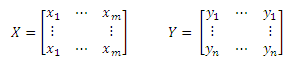
\includegraphics[width=150pt]{./Imagenes/matrices.png}
\end{center}


Es decir, las m filas de X son copias del vector x y las n columnas de Y son copias del vector y. La malla esta formada por los puntos $(X_{(i,j)},Y_{(i,j)})$. Por ejemplo,

\begin{lstlisting}[language=Matlab]
>> x=[0 0.33 0.67 1]; y=[-1 0 1];
>> [X,Y]=meshgrid(x,y)
X =
0 0.3300 0.6700 1.0000
0 0.3300 0.6700 1.0000
0 0.3300 0.6700 1.0000

Y =
-1 -1 -1 -1
 0  0  0  0
 1  1  1  1
\end{lstlisting}

Ahora para representar la superficie $z = f(x, y)$ utilizamos la orden \textbf{surf(X,Y,Z)} donde,

\begin{center}
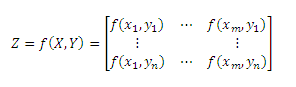
\includegraphics[width=150pt]{./Imagenes/matrices2.png}
\end{center}

A continuación vemos un ejemplo de superficie creada con el comando \textbf{surf}:

\begin{lstlisting}[language=Matlab]
>> x=linspace(-2,2,40);
>> y=linspace(-1,1,20);
>> [X,Y]=meshgrid(x,y);
>> Z=X.^2-Y.^2;
>> surf(X,Y,Z)
\end{lstlisting}
\begin{center}
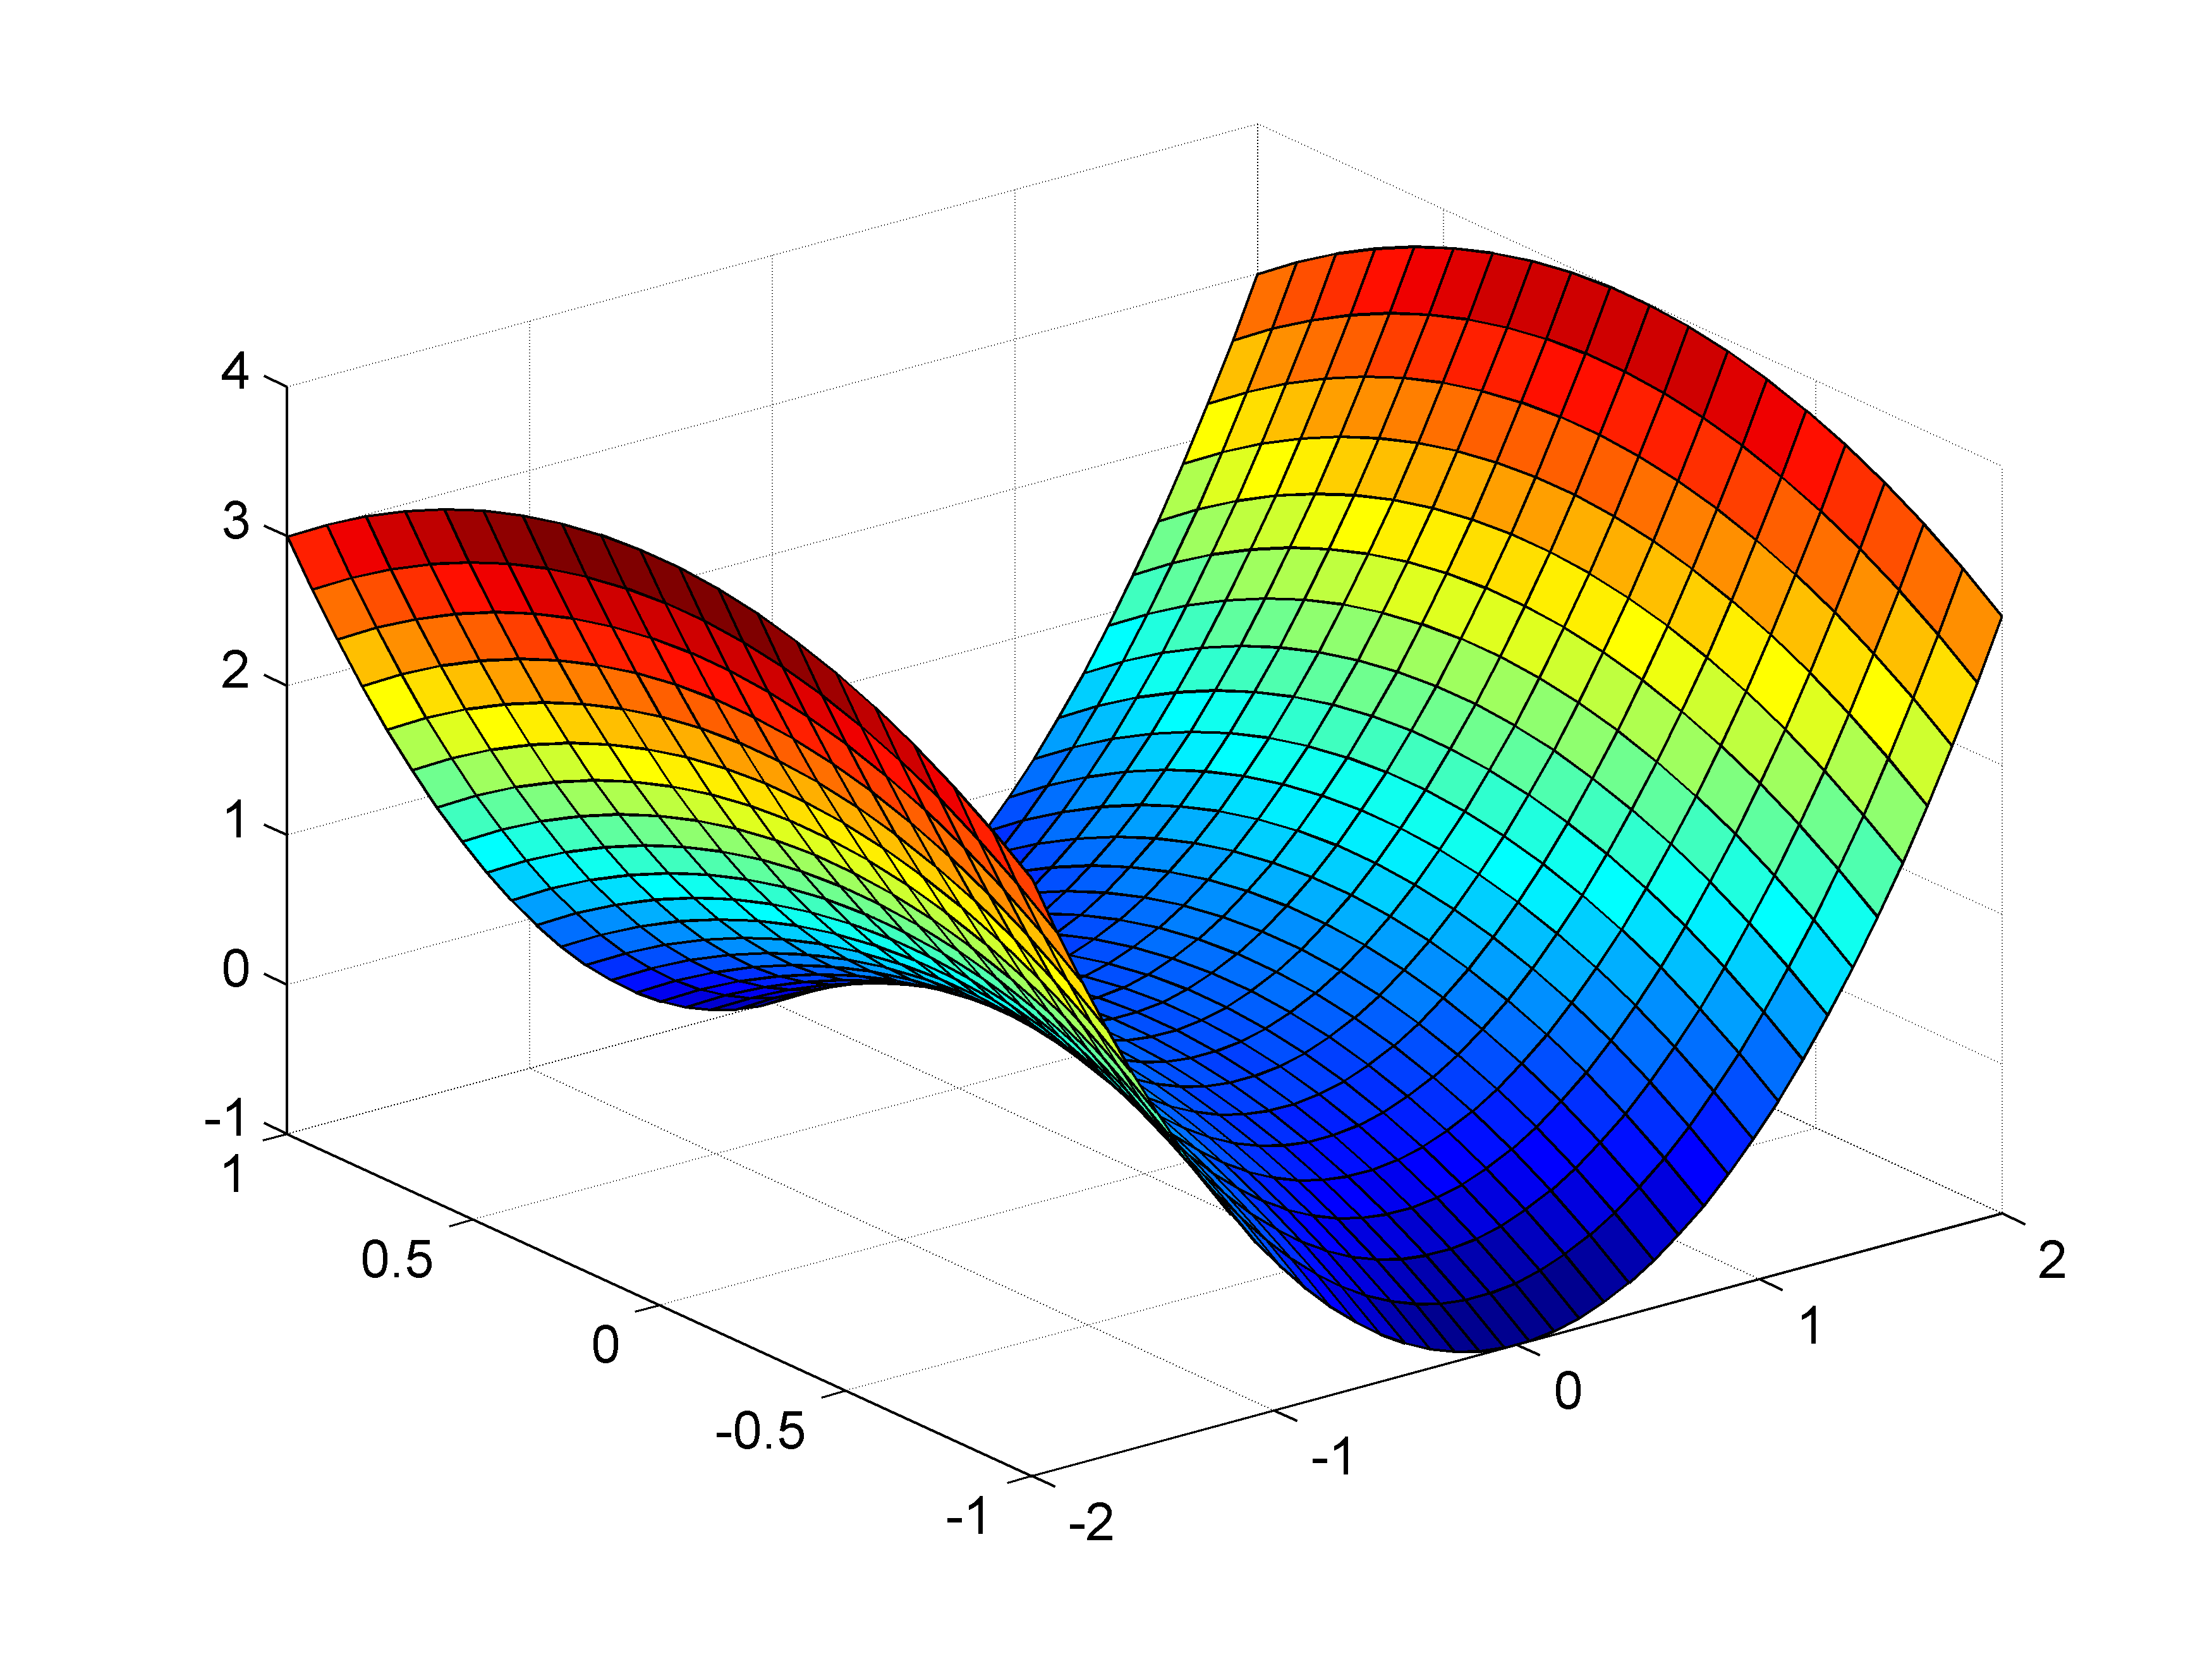
\includegraphics[width=300pt]{./Imagenes/surface1.png}
\end{center}

Se puede también dibujar una superficie y asignarle a esta un color según los valores de un cuarto vector.

\begin{lstlisting}[language=Matlab]
>> x=linspace(-3,3,60);
>> y=linspace(-3,3,60);
>> [X,Y]=meshgrid(x,y);
>> Z=X.^2-Y.^2;
>> T=cos(sqrt(X.^2+Y.^2+Z.^2));
>> surf(X,Y,Z,T), colorbar
\end{lstlisting}
\begin{center}
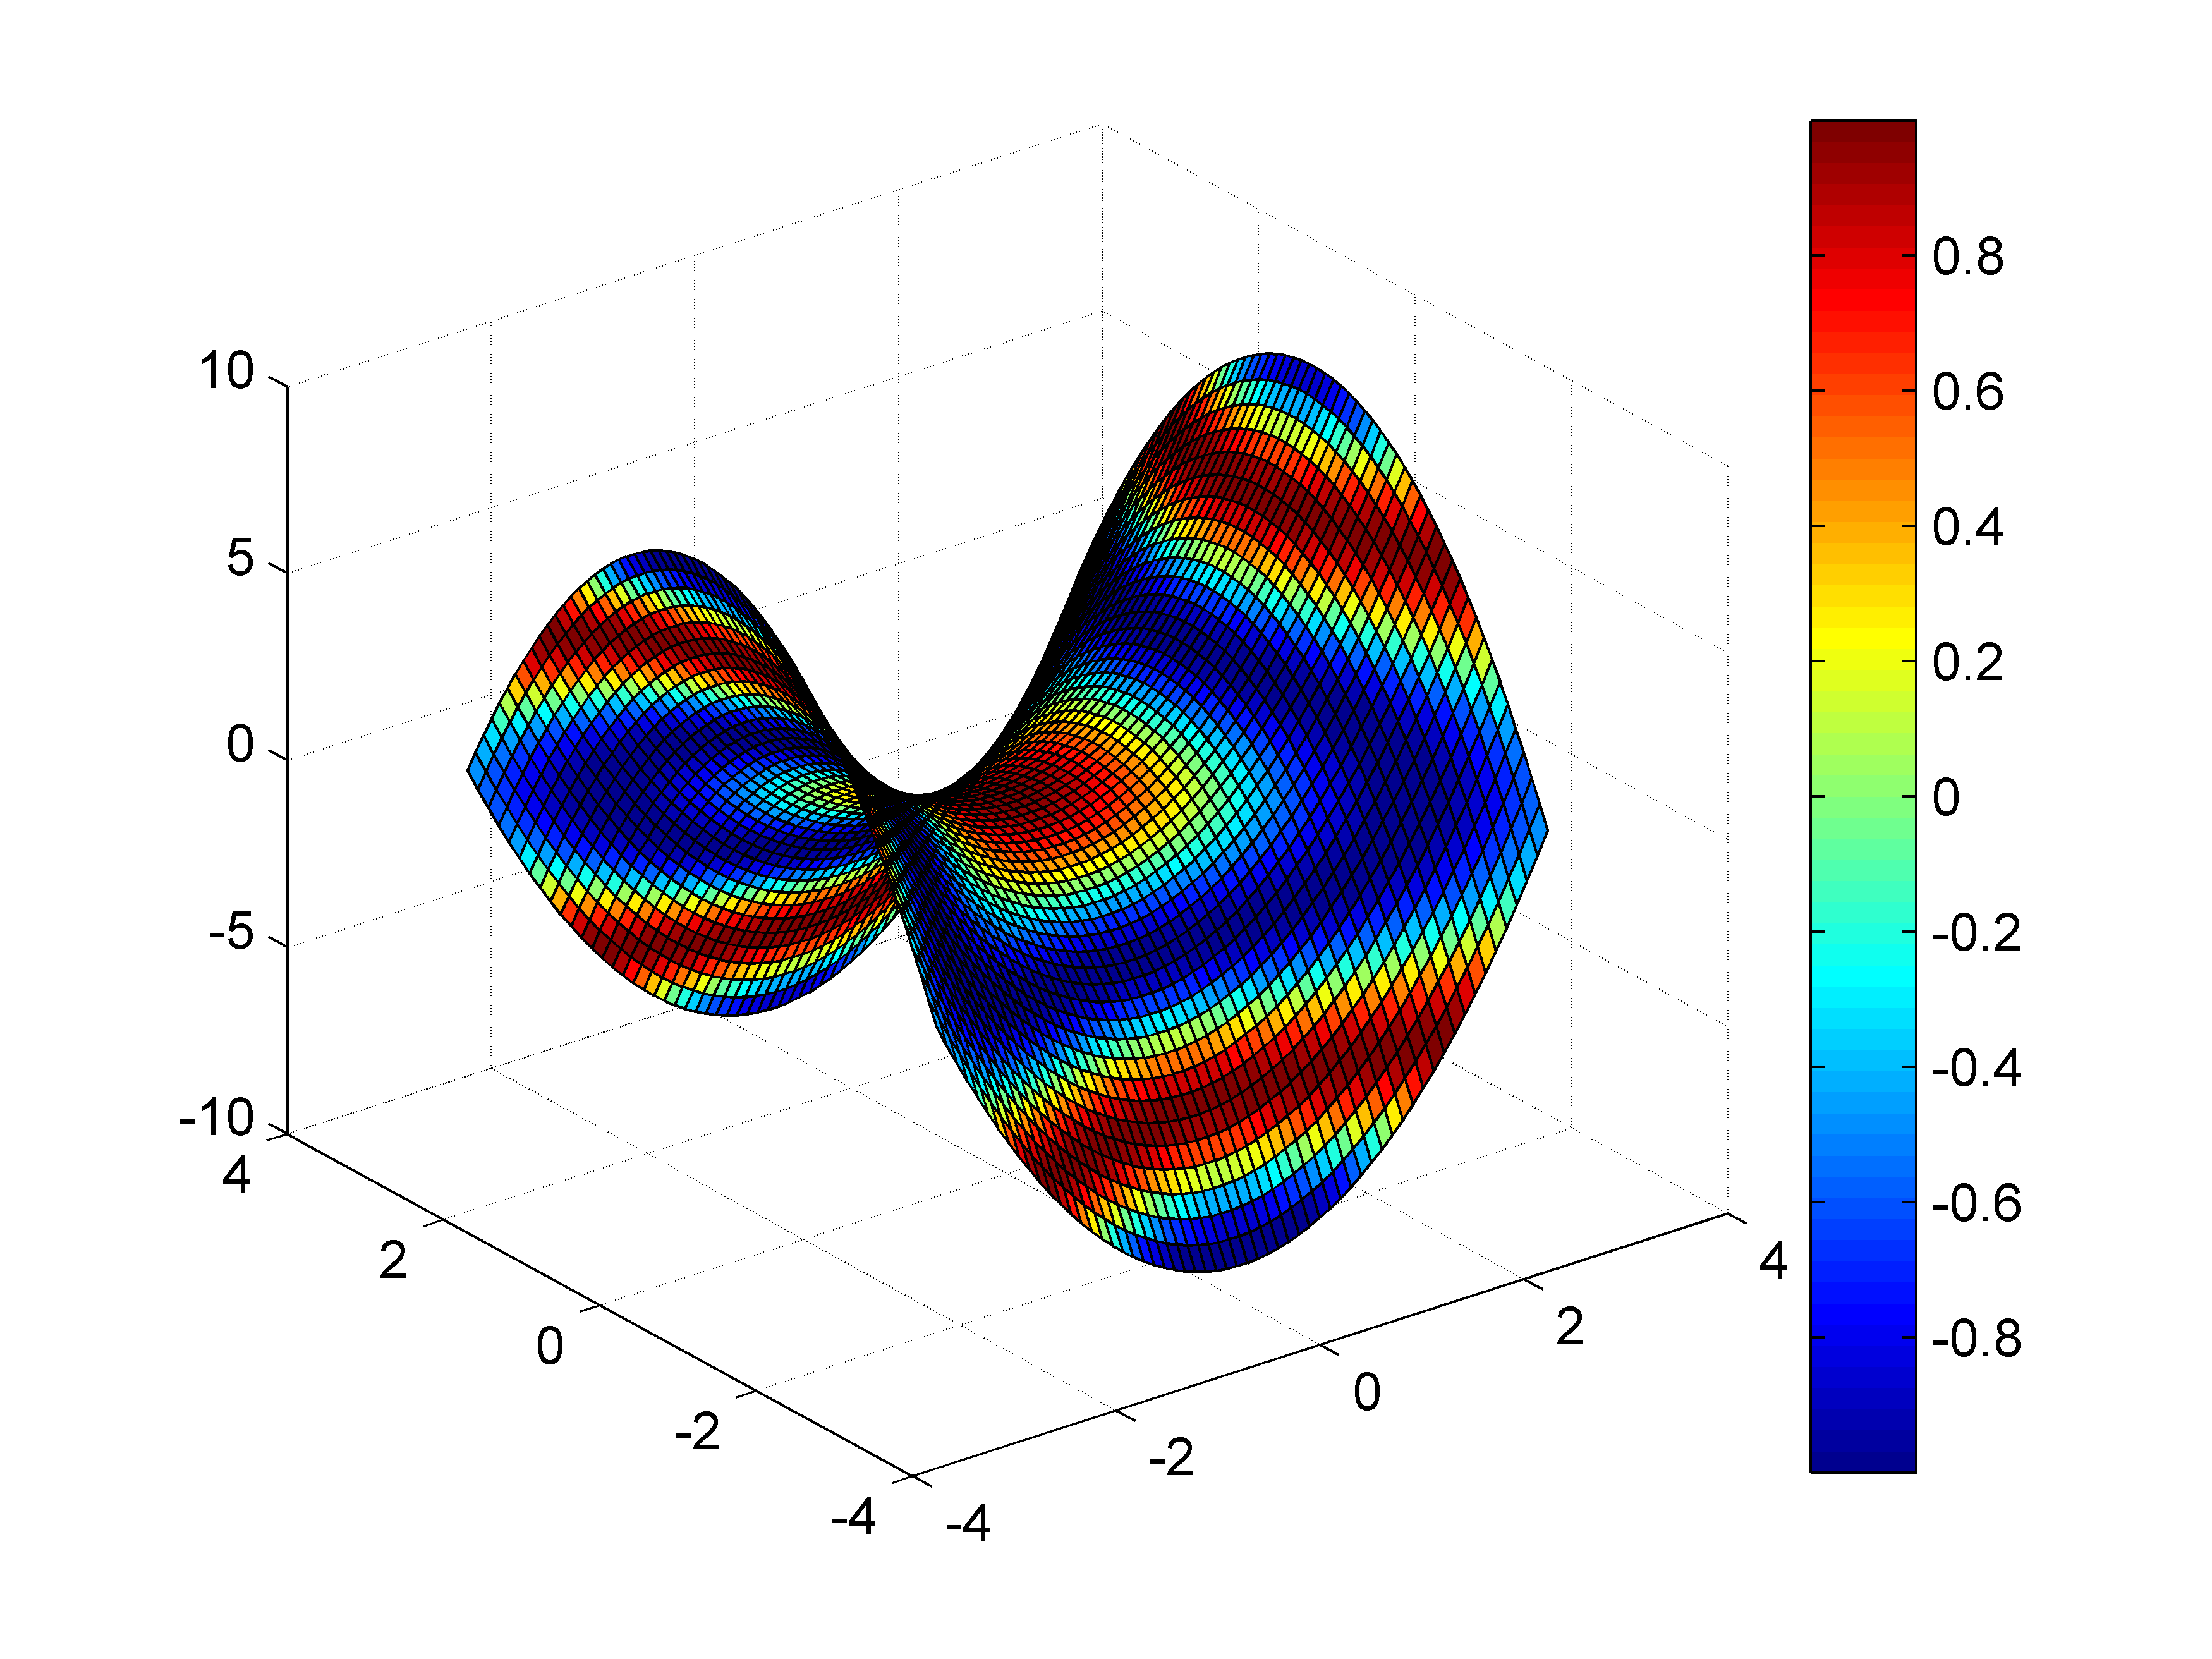
\includegraphics[width=300pt]{./Imagenes/surface2.png}
\end{center}

La orden $surf$ dibuja las superficies con colores sólidos. Se han introducido en la generación de las gráficas algunas especificaciones como:
\begin{lstlisting}[language=Matlab]
>> colormap(C) % Tabla de color usada para los graficos.
>> colorbar % Dibuja una barra de colores
>> shading flat % Quita la red del dibujo
>> shading interp % Varia el color en cada segmento
>> shading faceted % Defecto
\end{lstlisting}

A continuación se muestran algunos ejemplos de las gamas de colores que podemos usar junto al comando $colormap()$:
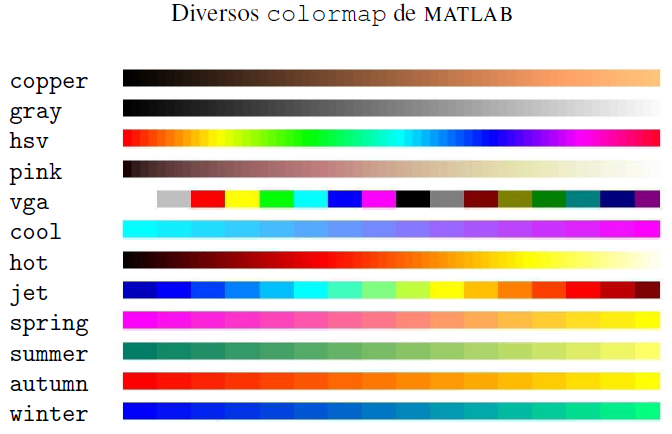
\includegraphics[width=300pt]{./Imagenes/3d4.png}

Ejemplo del uso del comando $surf$ con varias gráficas en una misma ventana:
\begin{lstlisting}[language=Matlab]
>> Z=membrane;
>> subplot(221), surf(Z)
>> subplot(222), surfc(Z)
>> subplot(223), surfc(Z), colorbar
>> subplot(224), surfc(Z), shading flat, colorbar
\end{lstlisting}

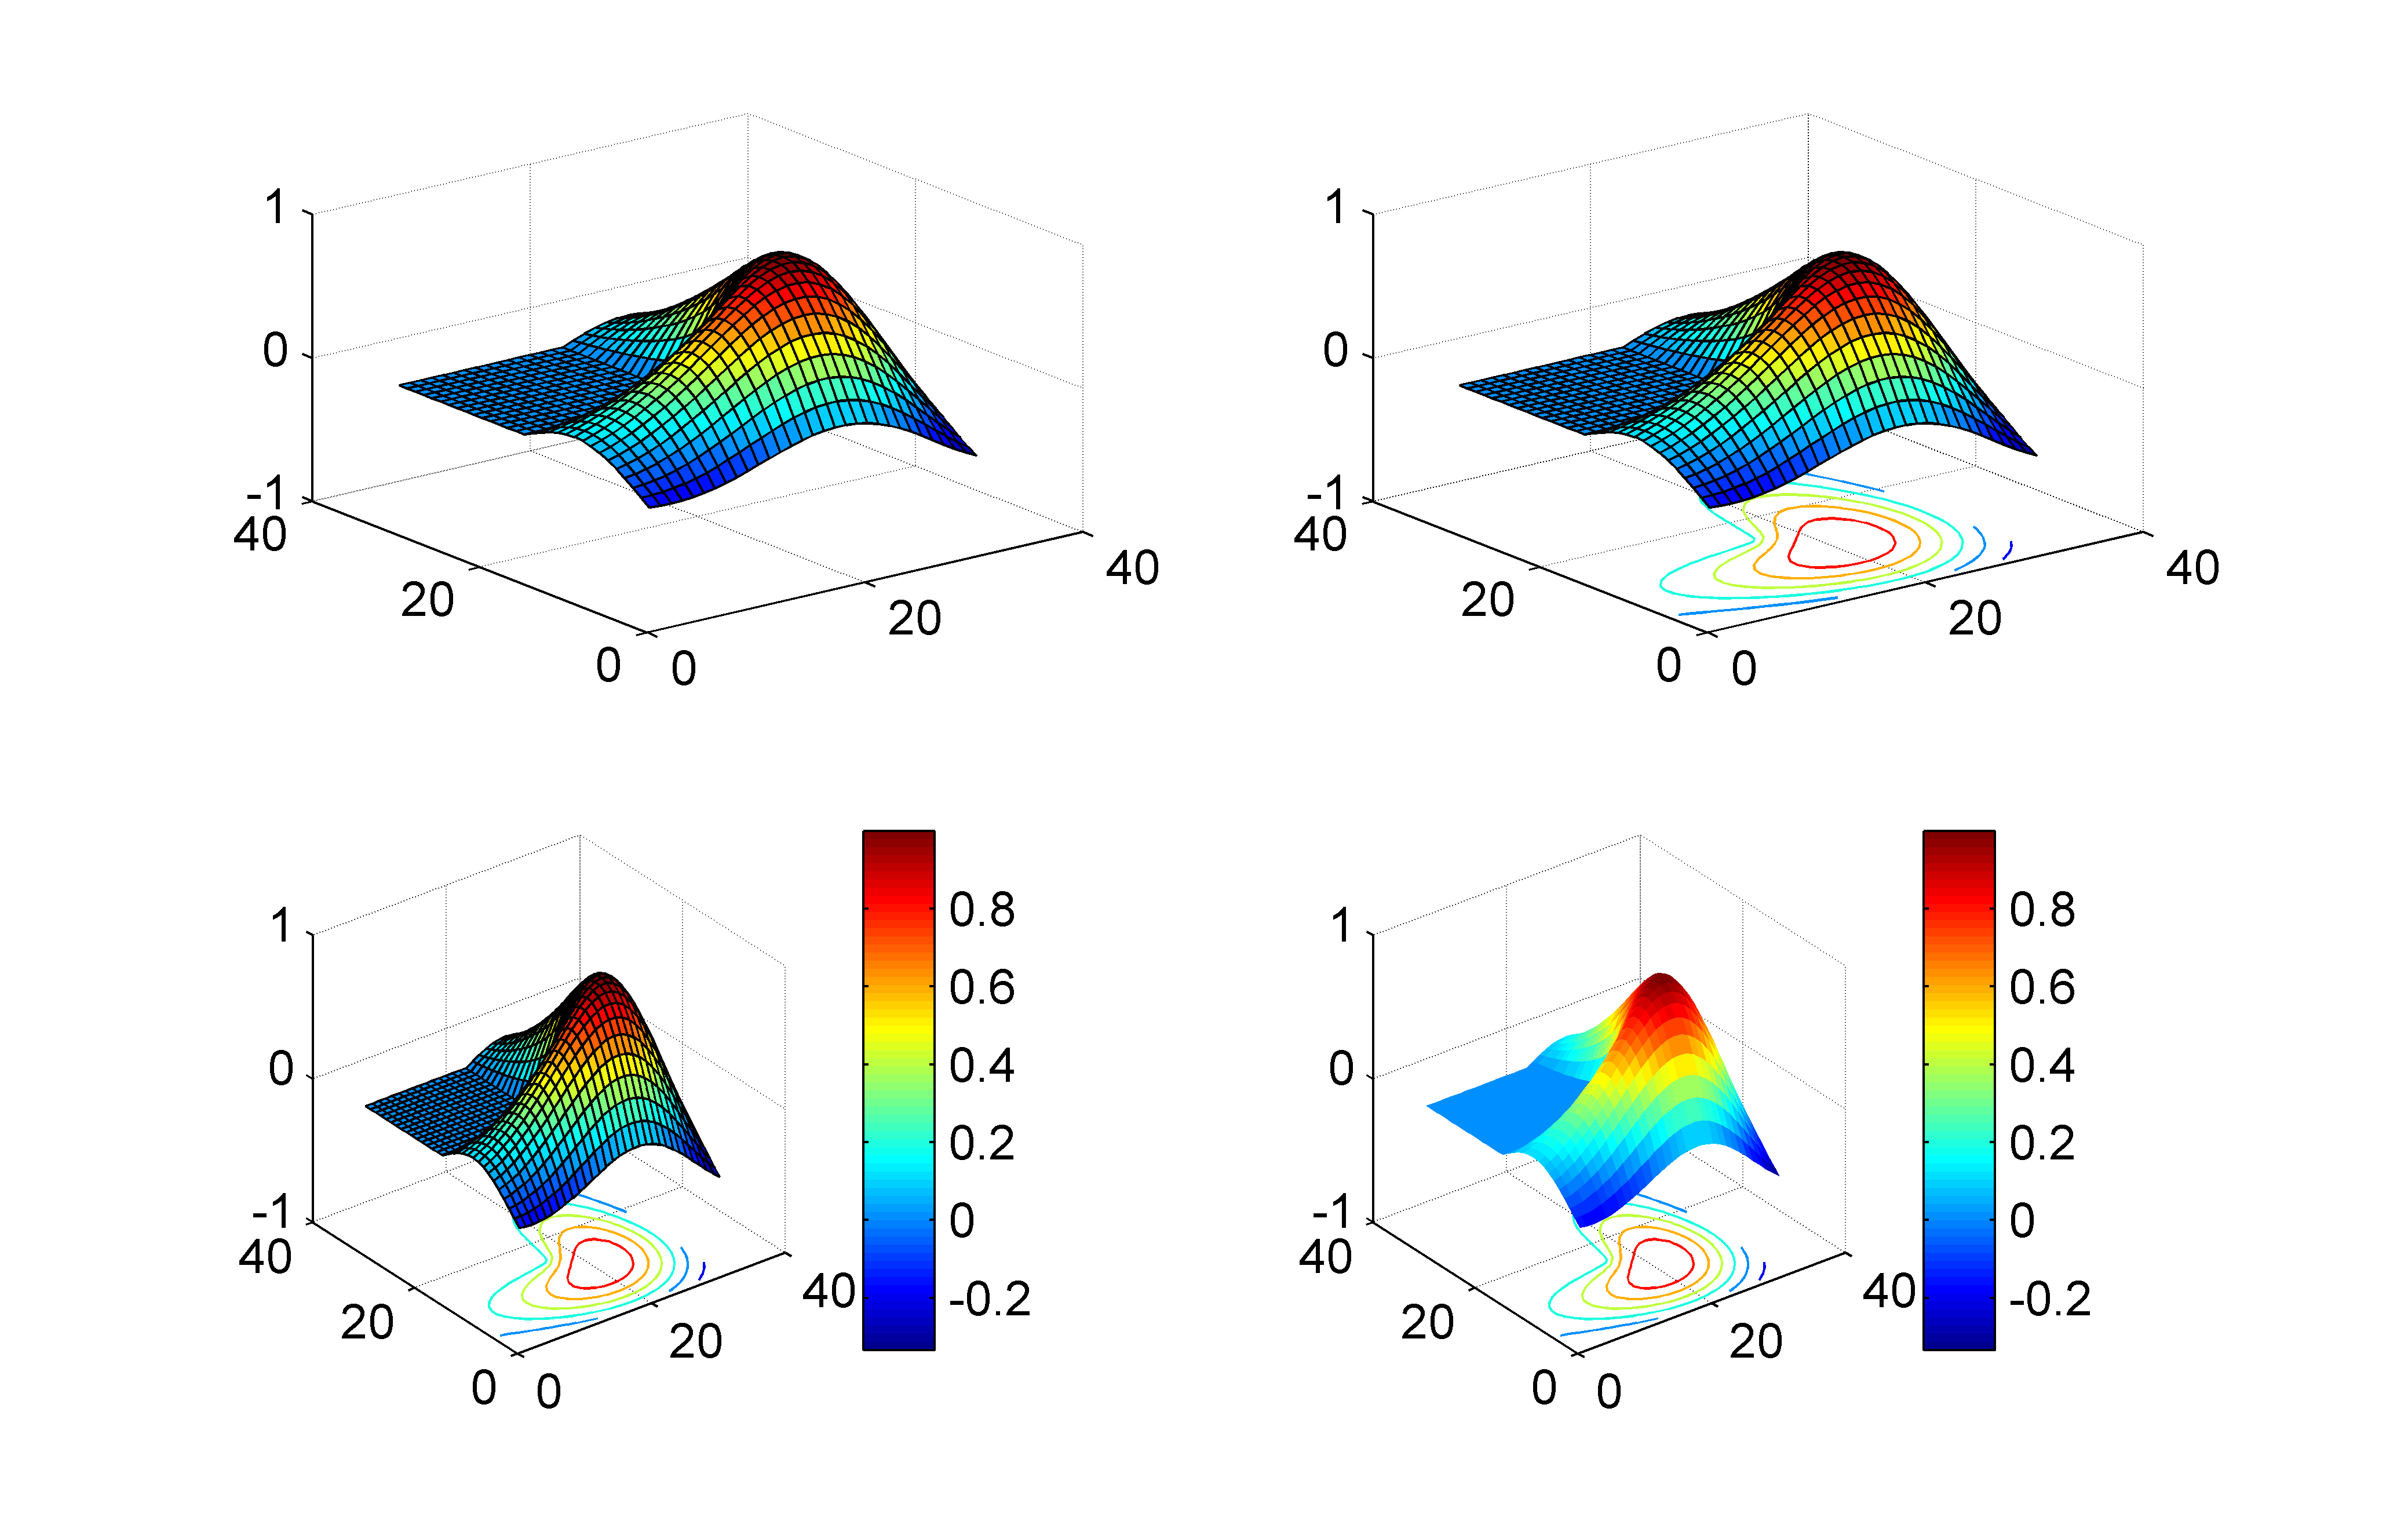
\includegraphics[width=400pt]{./Imagenes/3d5.png}

\section{Comandos de entorno 3D}

Hay 5 comandos importantes que describiremos a continuación. Sirven para manejar el entorno 3D, desde el color hasta el aspecto de la imagen.

\begin{itemize}
\item \textbf{colorbar}: despliega una barra de colores que informa sobre la correspondencia entre el valor numérico y el color utilizado. Por defecto aparece verticalmente a la derecha del dibujo aunque puede moverse posteriormente.
\item \textbf{colormap}: especifica que colores se van a utilizar en el dibujo. Existe un conjunto de formatos predefinidos listados a continuación. Para cambiar el formato de colores basta con utilizar el comando \textbf{colormap('opción')}:
\begin{itemize}
\item \textbf{autumn}
\item \textbf{gray}
\item \textbf{prism}
\item \textbf{bone}
\item \textbf{hot}
\item \textbf{spring}
\item \textbf{colorcube}
\item \textbf{hsv}
\item \textbf{summer}
\item \textbf{cool}
\item \textbf{jet}
\item \textbf{white}
\item \textbf{copper}
\item \textbf{lines}
\item \textbf{winter}
\item \textbf{flag}
\item \textbf{pink}
\item \textbf{default}
\end{itemize}

\item \textbf{daspect}: controla la relación entre los ejes del gráfico. Por ejemplo, mediante la siguiente instrucción se establece que los ejes X, Y y Z sean iguales. 
\begin{lstlisting}[language=Matlab]
>> daspect([1 1 1])
\end{lstlisting}

\item \textbf{pbaspect}: similar al comando anterior, pero este esta relacionado con la caja que enmarca al gráfico.
\item \textbf{view}: especifica desde donde se ve el gráfico. El comando tiene dos parámetros:
\begin{lstlisting}[language=Matlab]
>> view(az,el)
\end{lstlisting}
El primer parámetro es azimuth (angulo de rotación horizontal) y el segundo parámetro es el angulo de elevación vertical. Estos dos parámetros se deben especificar en grados. Por defecto, \textbf{MATLAB} le asigna a los gráficos 3D los valores de az=-37.5 y el=30.
\end{itemize}

\section{Comandos contour y mesh}
Para dibujar una superficie $z = f(x,y)$ en un dominio $D = [x_{0}, x_{f}] * [y_{0}, y_{f}]$, primero hay que definir una malla con el comando $meshgrid$ y luego evaluar $z = f(x, y)$ en dicha malla.
\begin{lstlisting}[language=Matlab]
>> [X,Y]=meshgrid( x0:xpaso:xf, y0:ypaso:yf);
>> Z=f(X,Y);
\end{lstlisting}

Las ordenes de dibujo 3D más usuales son:
\begin{lstlisting}[language=Matlab]
>> contour(X,Y,Z,num) - Genera las curvas de nivel
>> mesh(X,Y,Z) - Dibuja la  Z (ejes cartesianos)
>> meshc(Z) - mesh + contour (ejes matriciales)
>> meshc(X,Y,Z) - mesh + contour (ejes cartesianos)
>> surf(Z) - Dibujo solido (ejes matriciales)
>> surf(X,Y,Z) - Dibujo solido (ejes cartesianos)
\end{lstlisting}

Veamos un ejemplo de dibujo de curvas de nivel con la orden contour:
\begin{lstlisting}[language=Matlab]
>> [X,Y]=meshgrid( -4:0.1:4, -4:0.1:4);
>> Z= sin(X + Y.^2/10) + cos(X.^2-Y) + 0.5;
>> % Dibujo por defecto. (Ejes cartesianos)
>> subplot(221)
>> contour(X,Y,Z)
>> % Dibujar 5 curvas de nivel con relleno.
>> subplot(222)
>> contourf(X,Y,Z,5)
>> % Dibujar valores determinados de las curvas de
>> % nivel y etiquetarlos
>> subplot(223)
>> val = [-1 0 1. 2.];
>> [C,h] = contour(X,Y,Z,val);
>> clabel(C,h,val);
>> % Forma sencilla de dibujar curvas de nivel.
>> subplot(224)
>> ezcontour('sin(x+y^2/10)+cos(x^2-y)+.5',[-4,4,-4,4]);
\end{lstlisting}
\begin{center}
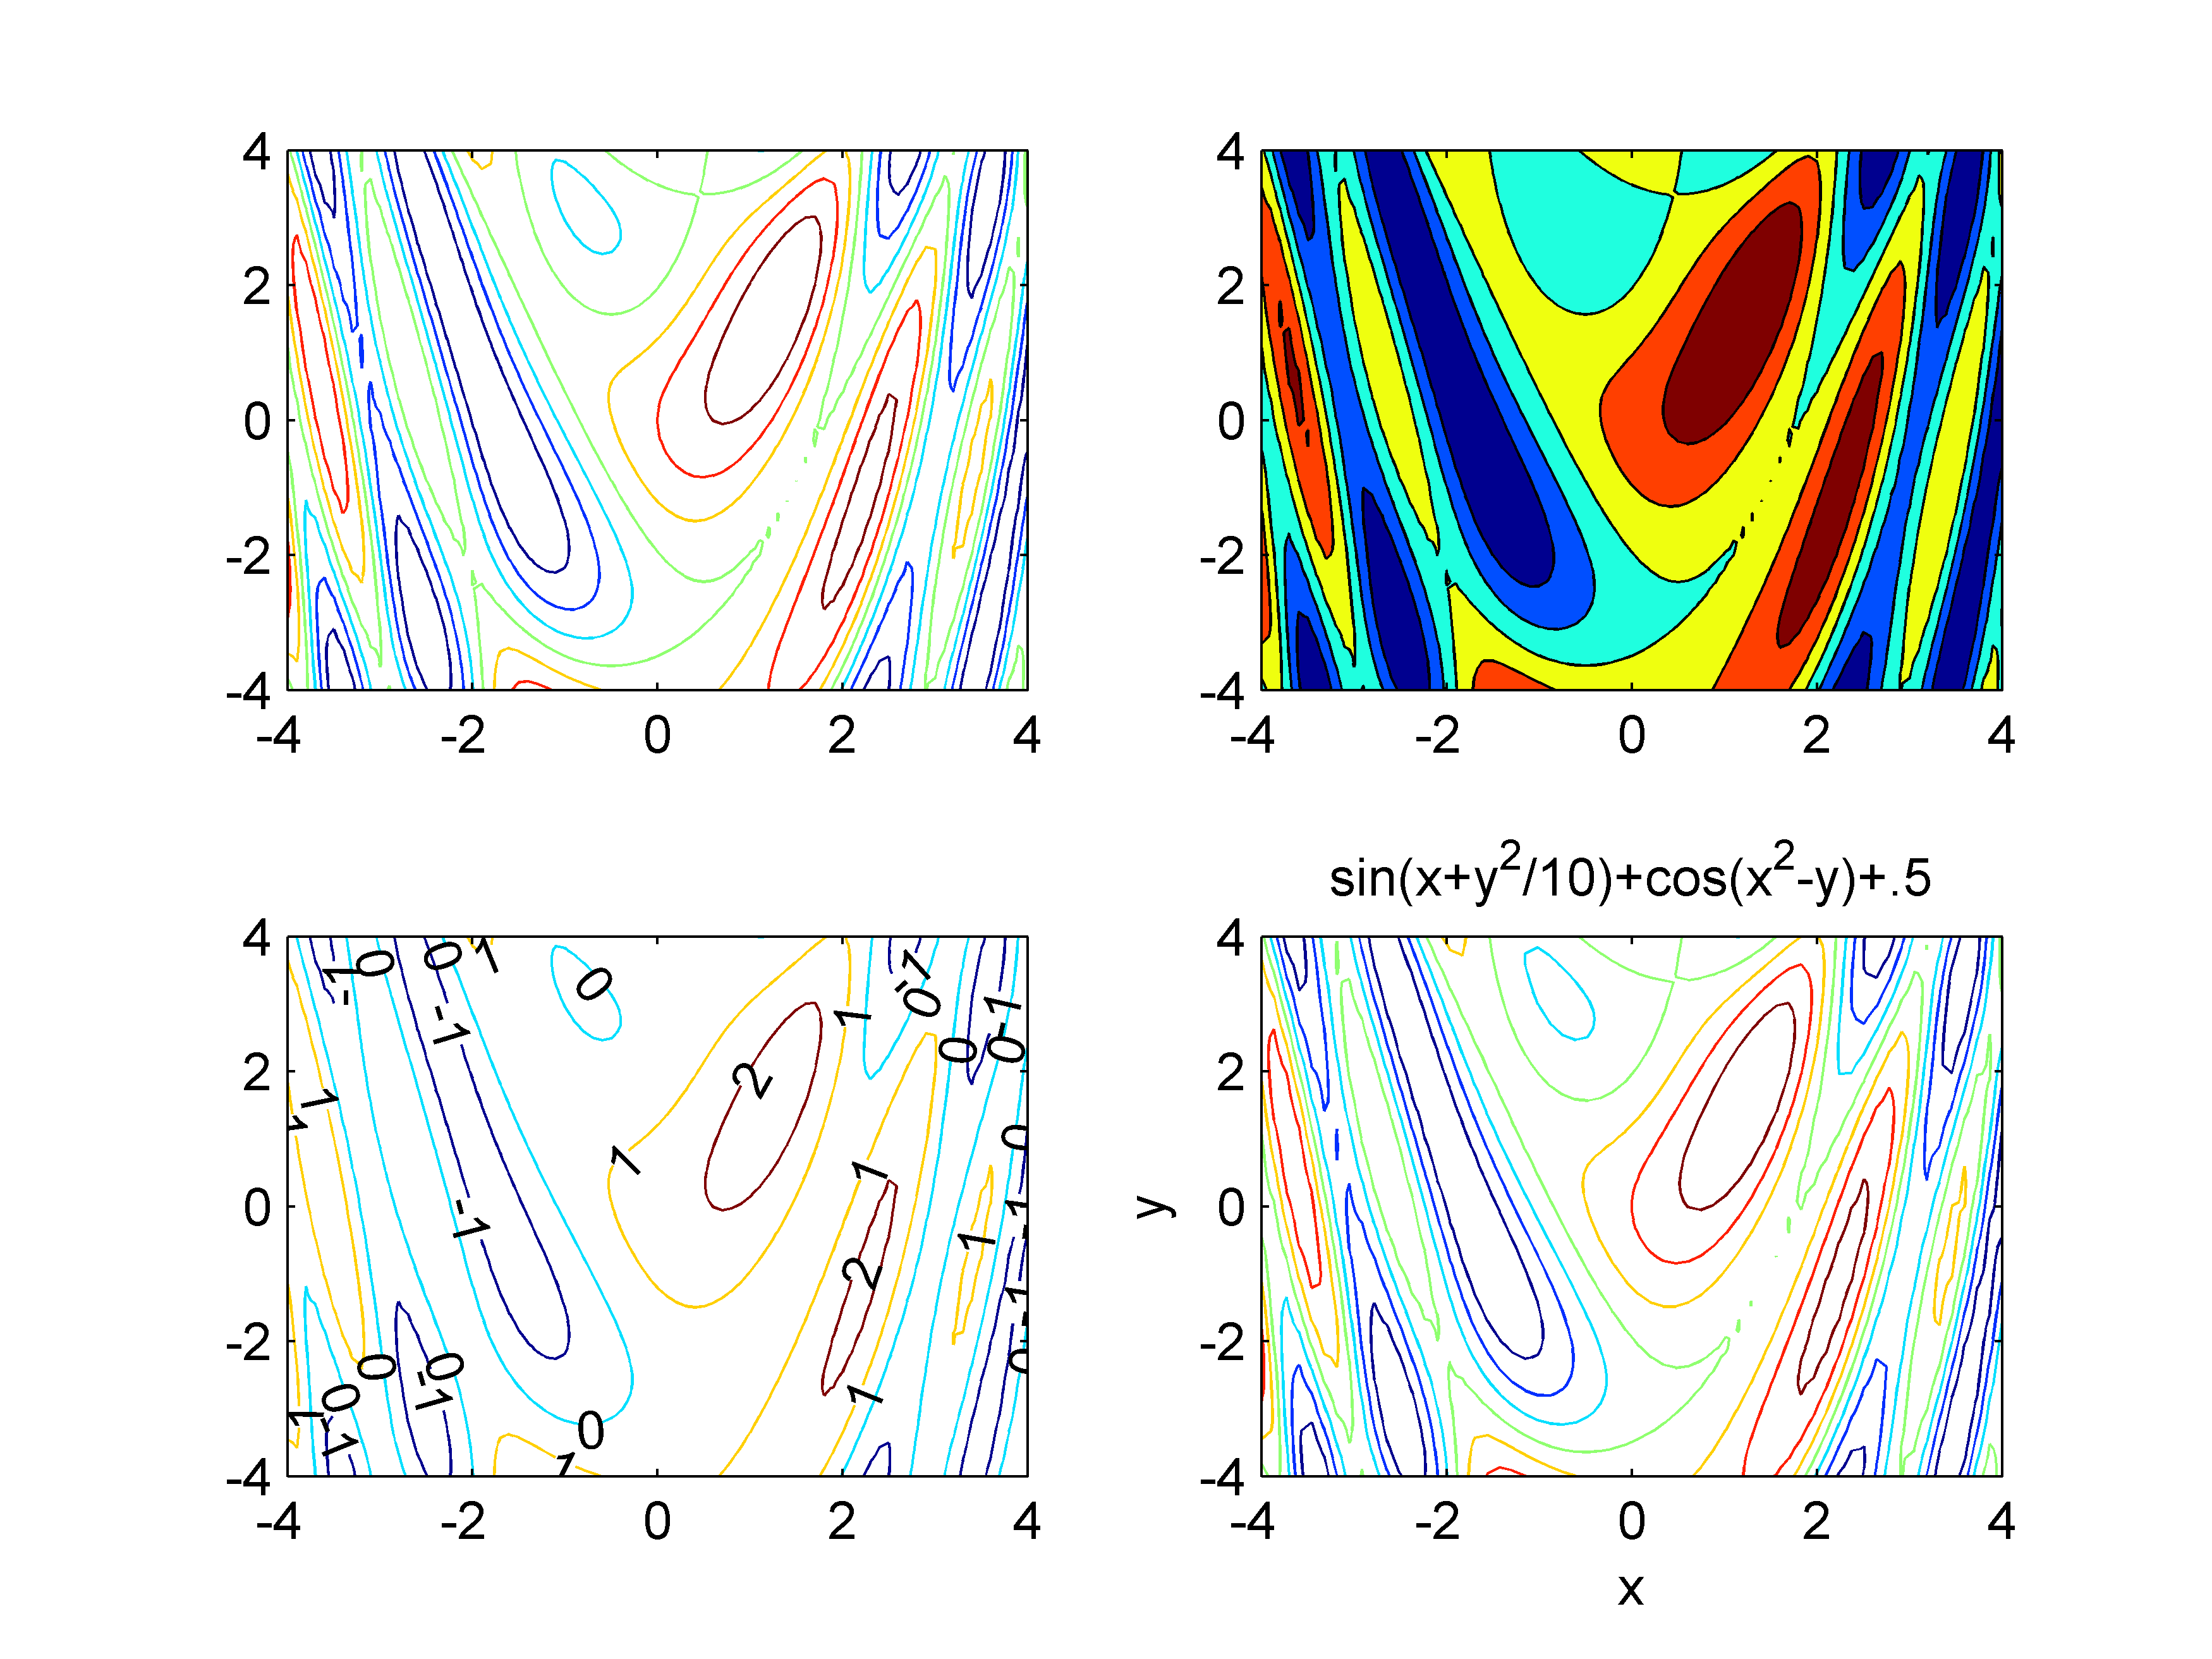
\includegraphics[width=300pt]{./Imagenes/3d2.png}
\end{center}

\subsection{Comando mesh}

La orden $mesh$ dibuja la superficie como si fuera una malla, veamos un ejemplo:
\begin{lstlisting}[language=Matlab]
>> [X,Y]=meshgrid( -4:0.5:4, -4:0.5:4);
>> Z= sin(X).*cos(Y);
>> subplot(221)
>> meshc(X,Y,Z)
>> xlabel('\bf x'); ylabel('\bf y'); zlabel('\bf z');
>> subplot(222)
>> mesh(X,Y,Z)
>> subplot(223)
>> mesh(X,Y,Z) % ejes cartesianos
>> axis([-6 6 -6 6 -4 4]);
>> subplot(224)
>> mesh(Z) % ejes matriciales
\end{lstlisting}
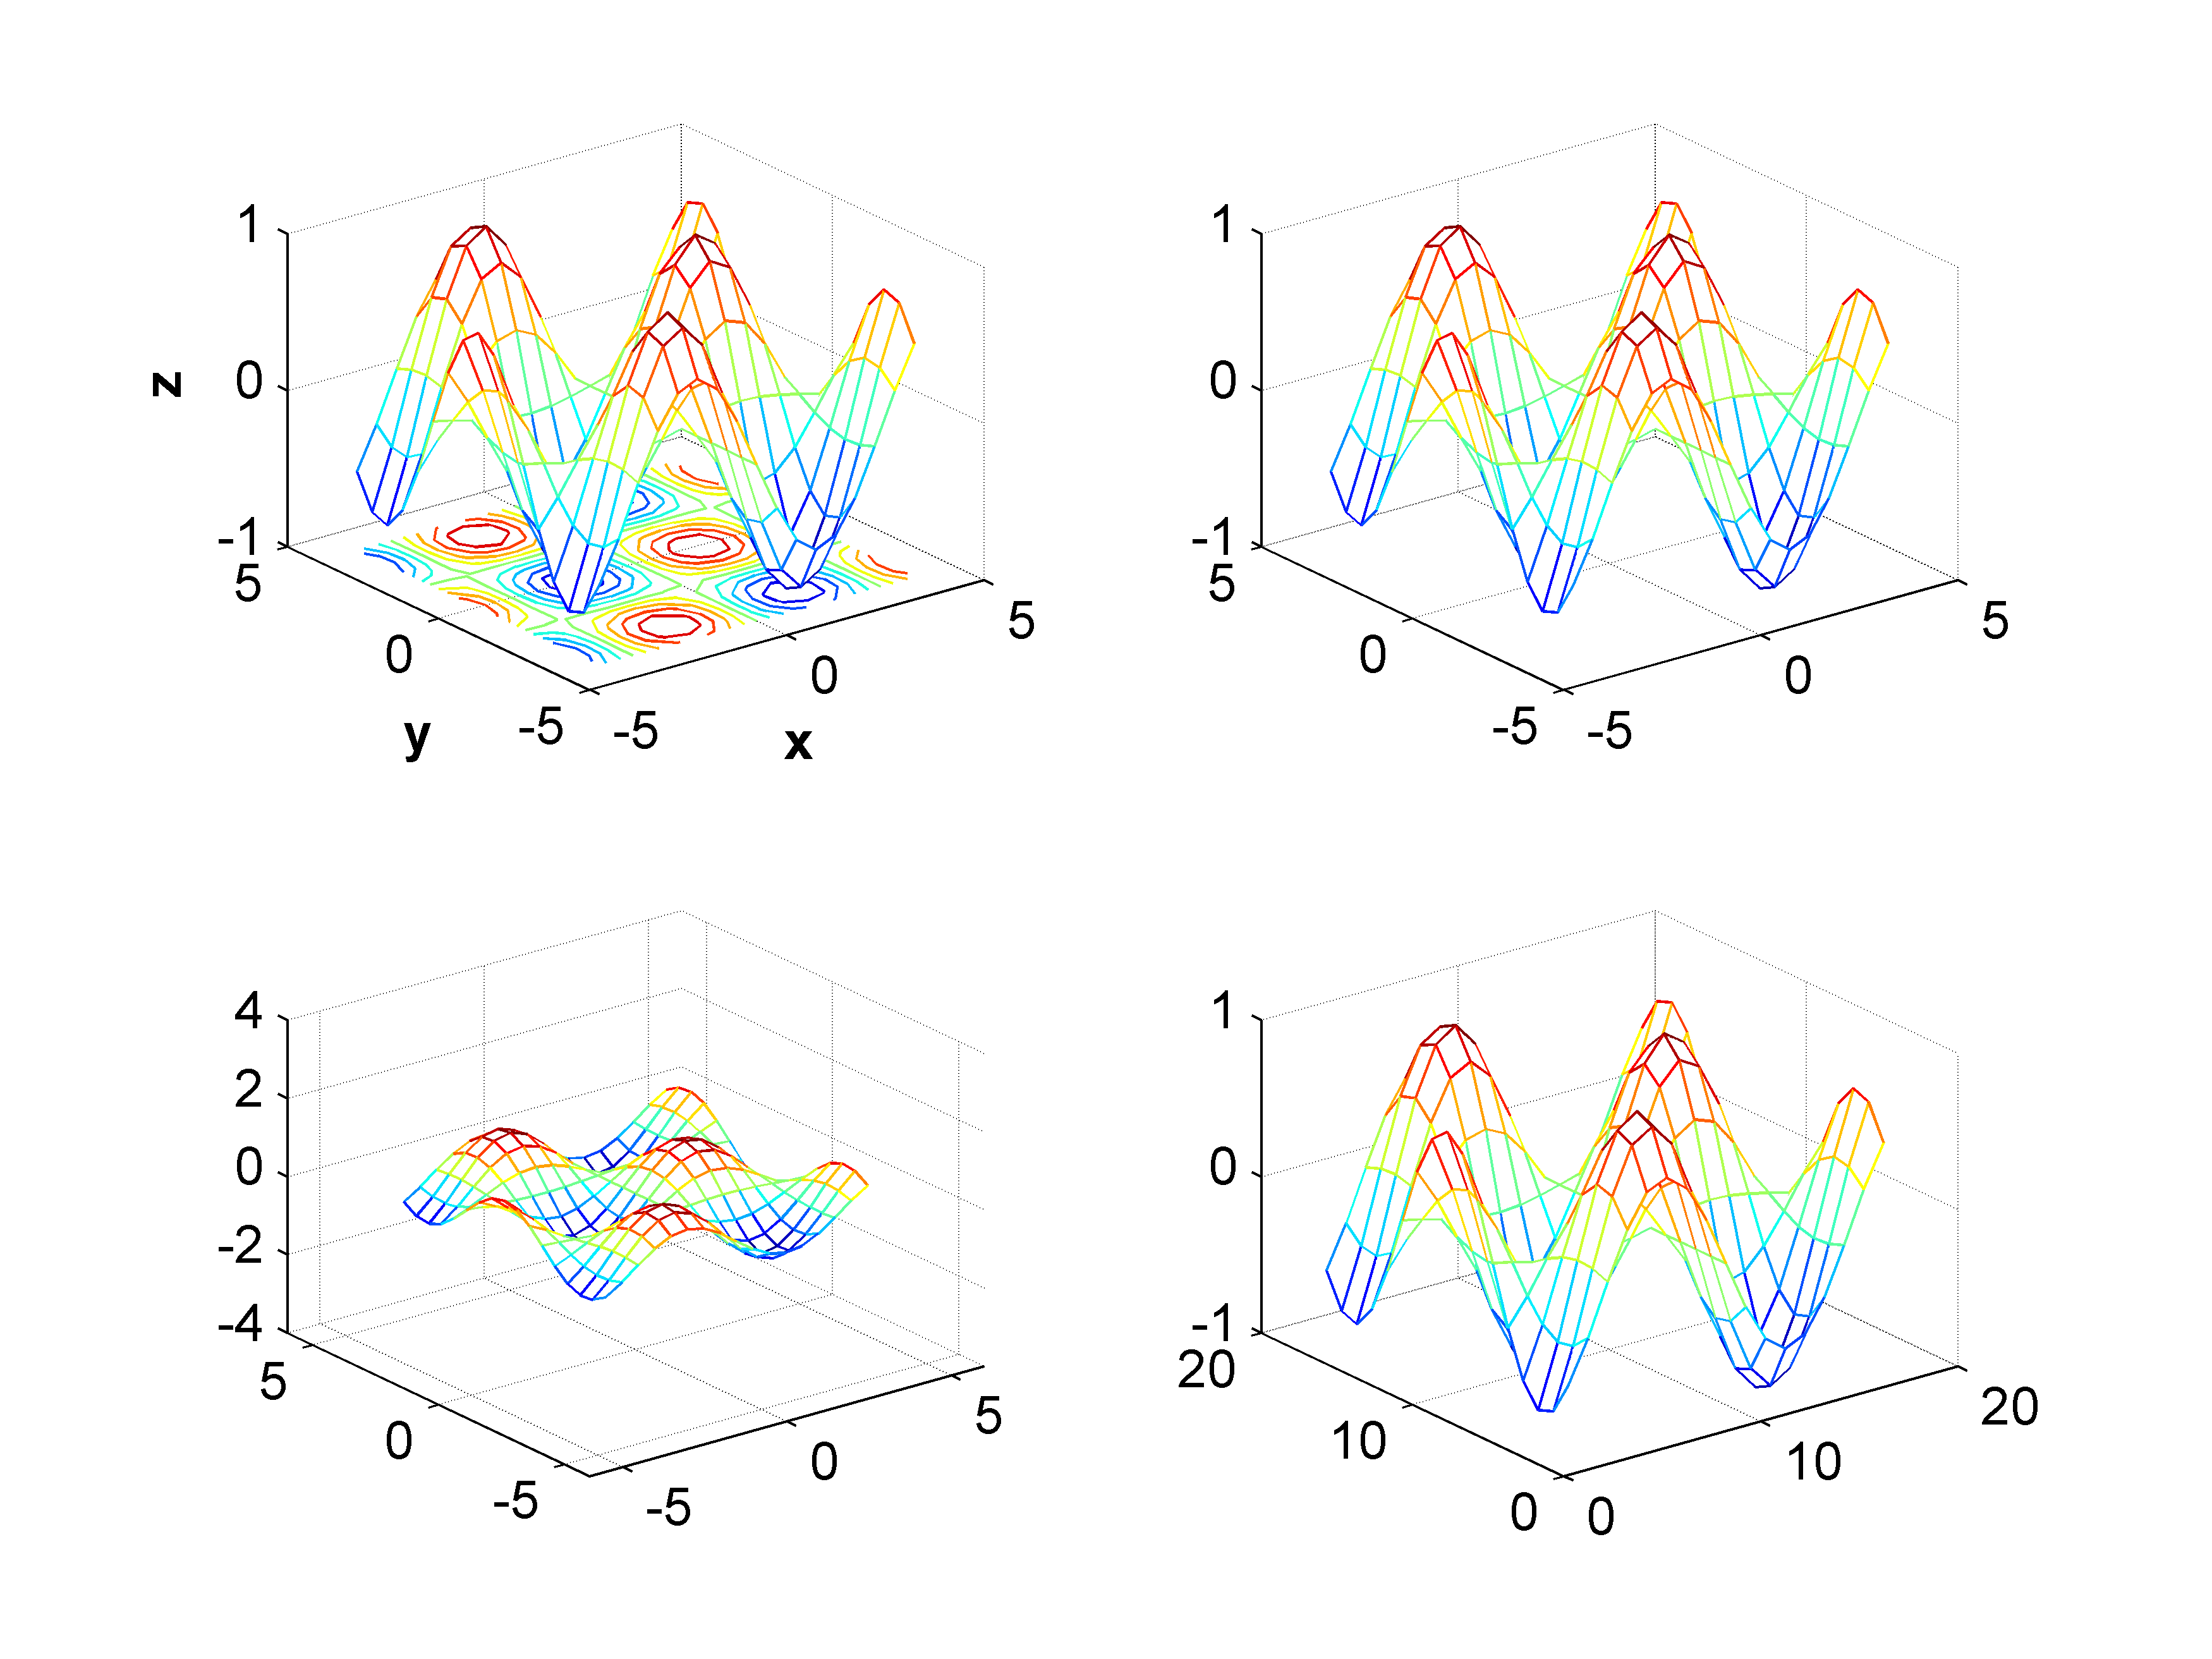
\includegraphics[width=300pt]{./Imagenes/3d3.png}


\section{Complementos}

La sentencia $surf$ puede utilizarse con cuatro parámetros (X,Y,Z,C), donde C representa la escala de color. \textbf{MATLAB} escala C para obtener los colores del actual colormap. Si solo hay tres parámetros, entonces $C=Z$, es decir el color es proporcional a la altura. Esto puede aprovecharse para representar una función $g(x, y, z)$ sobre la superficie definida por $(x, y, z)$.

\paragraph{Ejemplo 1}:
\begin{lstlisting}[language=Matlab]
>> [X,Y]=meshgrid(-3:0.05:3,-3:0.05:3);
>> Z=exp(-X.^2-Y.^2);
>> surf(X,Y,Z, X.^2+Y.^2+Z.^2), shading interp
>> colorbar
\end{lstlisting}
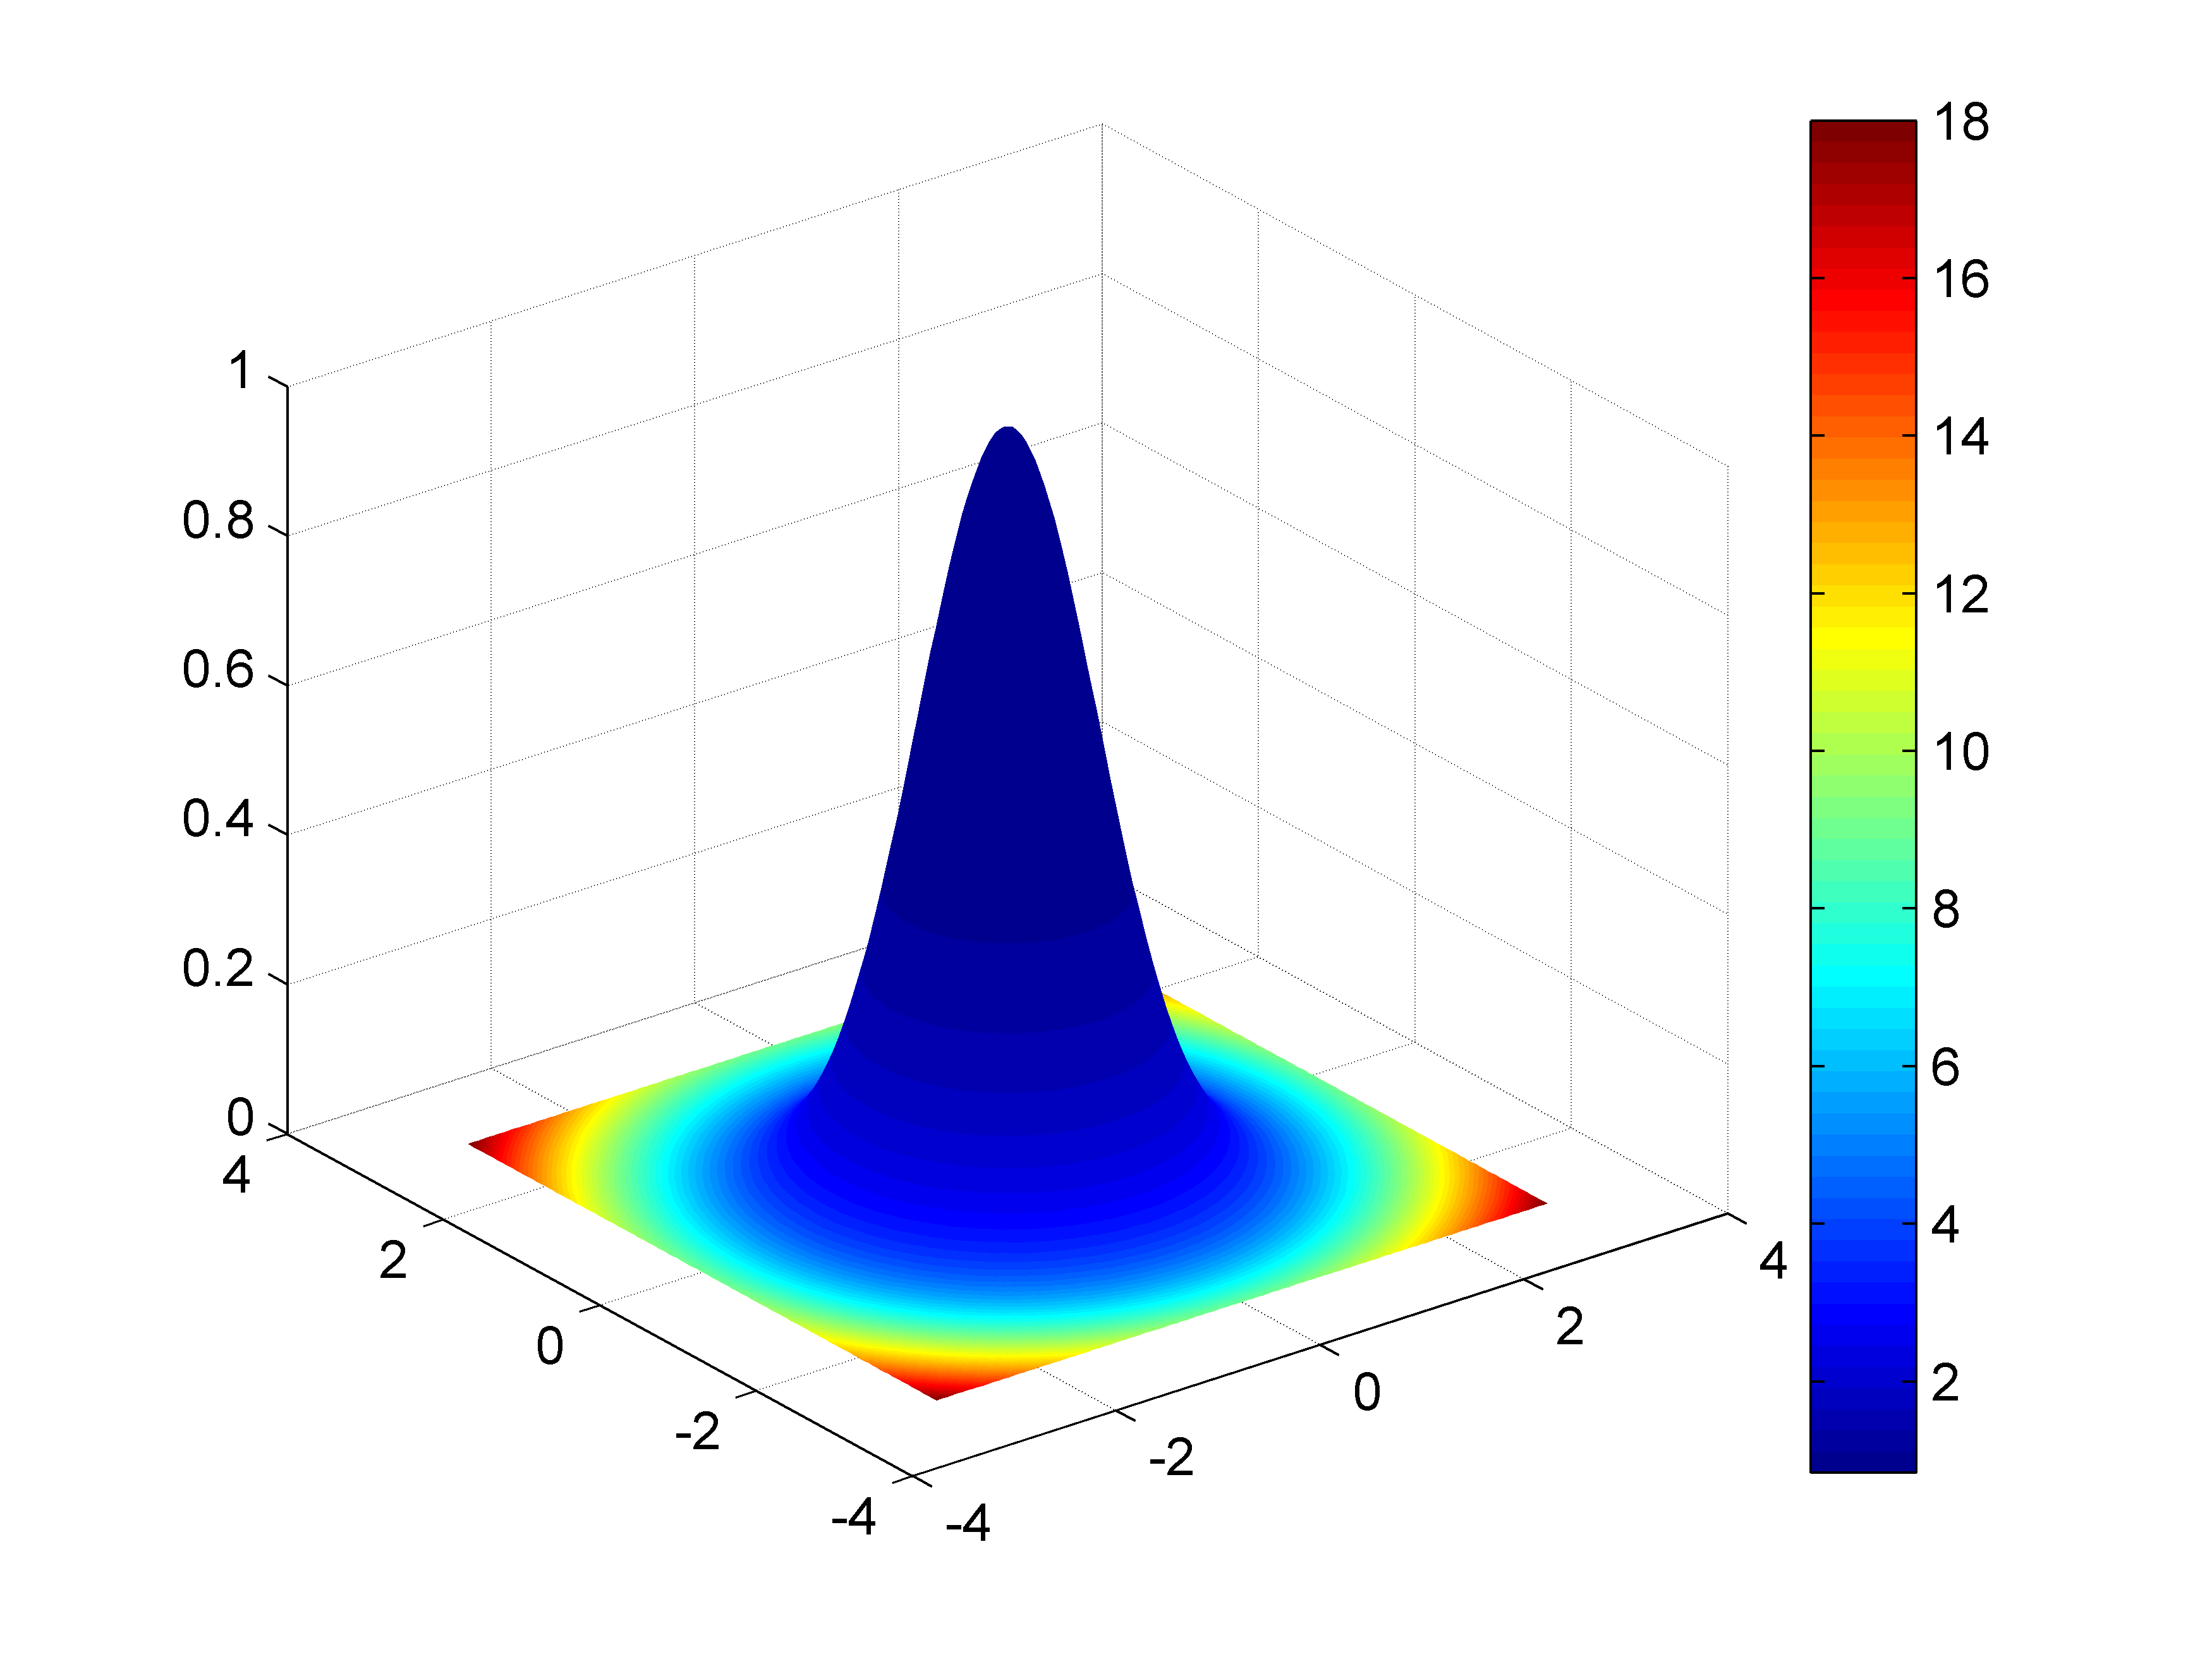
\includegraphics[width=300pt]{./Imagenes/3d6.png}

\paragraph{Ejemplo 2}:
\begin{lstlisting}[language=Matlab]
>> [X,Y]=meshgrid(-3:0.05:3,-3:0.05:3);
>> Z=cos(X).*cos(Y); Z(X.*Y > 2 & X.*Y<3)=NaN;
>> surf(X,Y,Z, X+Y+Z), shading interp
>> colormap('copper'); colorbar
\end{lstlisting}
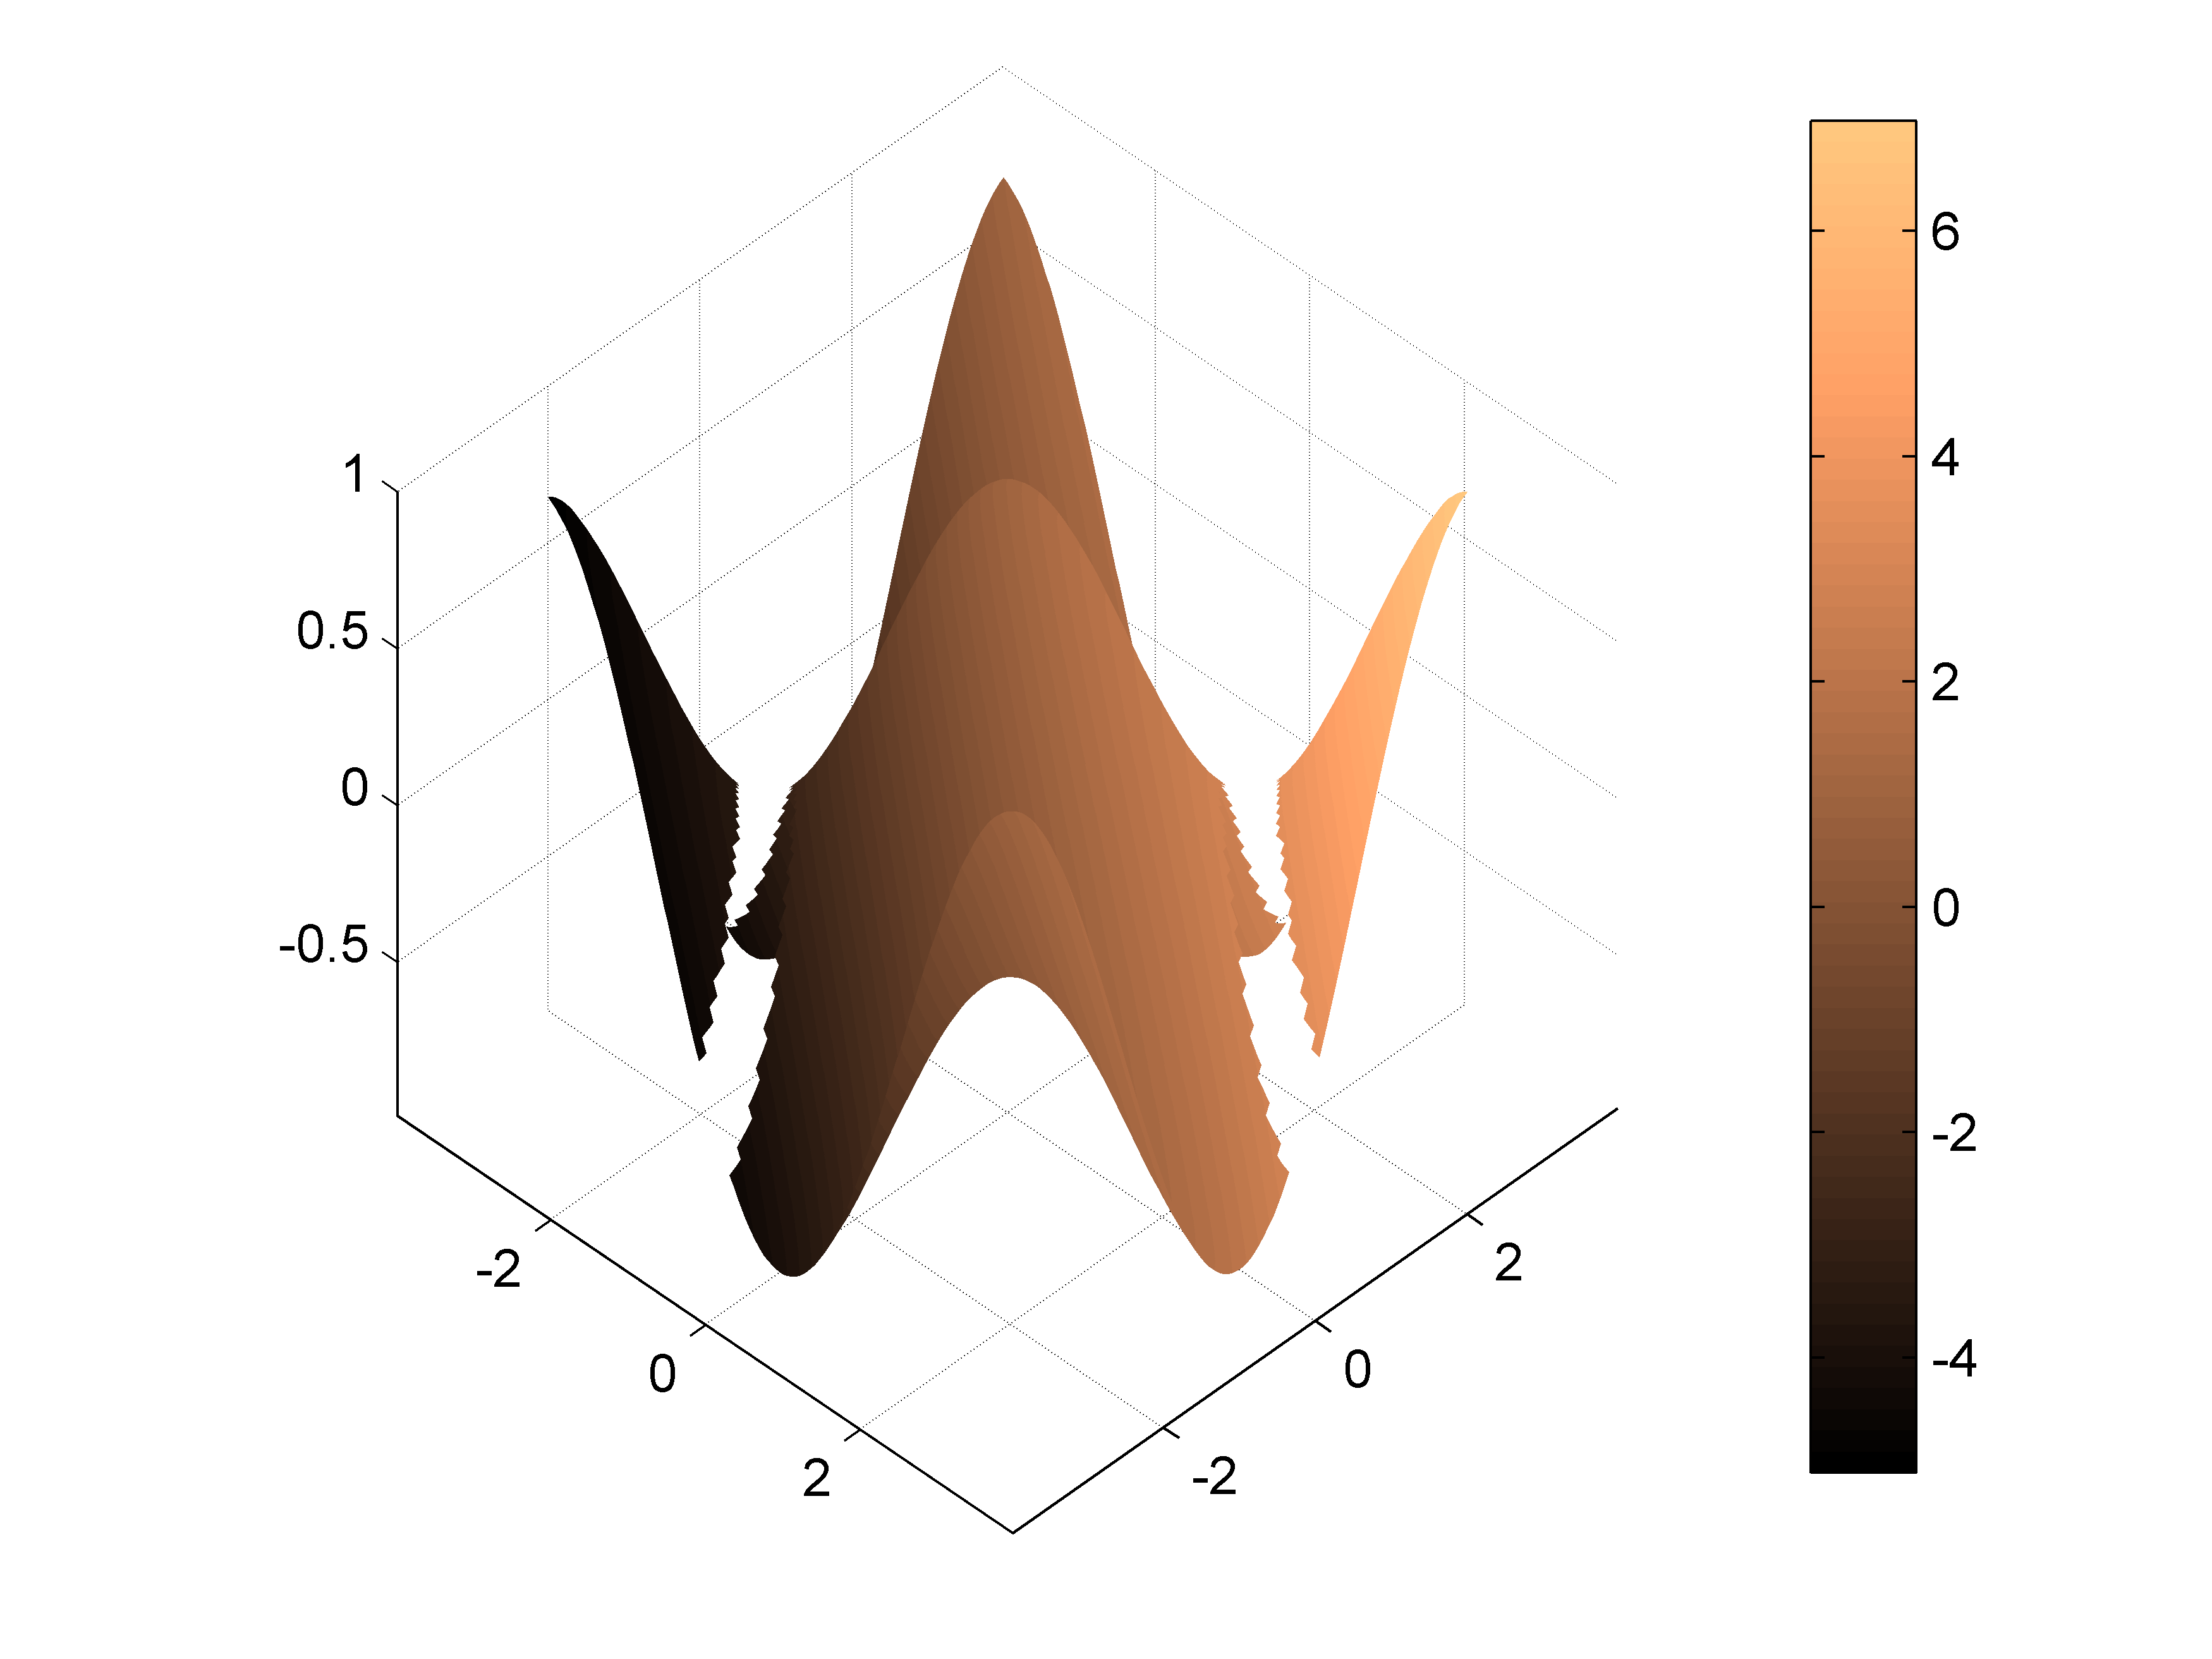
\includegraphics[width=300pt]{./Imagenes/3d7.png}

\paragraph{Ejemplo 3}:
\begin{lstlisting}[language=Matlab]
>> [X,Y]=meshgrid(-3:0.2:3); Z=exp(-X.^2-Y.^2);
>> surf(X,Y,Z, gradient(Z)), shading interp, colorbar
\end{lstlisting}
\includegraphics[width=300pt]{./Imagenes/3d8.png}

\paragraph{Ejemplo 4}:
\begin{lstlisting}[language=Matlab]
>> [X,Y]=meshgrid(-3:0.2:3); Z=exp(-X.^2-Y.^2);
>> surf(X,Y,Z,gradient(Z)), shading interp, alpha(0.6)
\end{lstlisting}
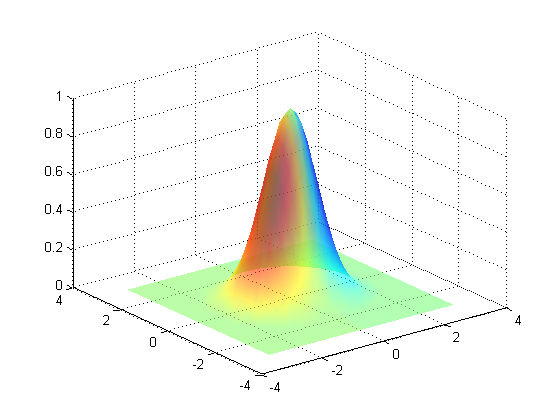
\includegraphics[width=300pt]{./Imagenes/3d9.png}

\section{Curvas de intersección entre dos superficies}

Existen muchos casos donde no se puede visualizar la curva que resulta de la intersección de 
dos superficies. Ejemplos:

\begin{enumerate}
\item La intersección de los cilindros: $z=x^{2}$ , $z=4-y^{2}$ es una curva en el espacio. Vamos a representar las dos superficies y luego su curva intersección. Gráfica de las superficies 

\begin{lstlisting}[language=Matlab]
>> [x,y]=meshgrid(-2:0.1:2); 
>> z=x.^2; mesh(x,y,z) 
>> hold on 
>> z=4-y.^2;
>> mesh(x,y,z)
\end{lstlisting}
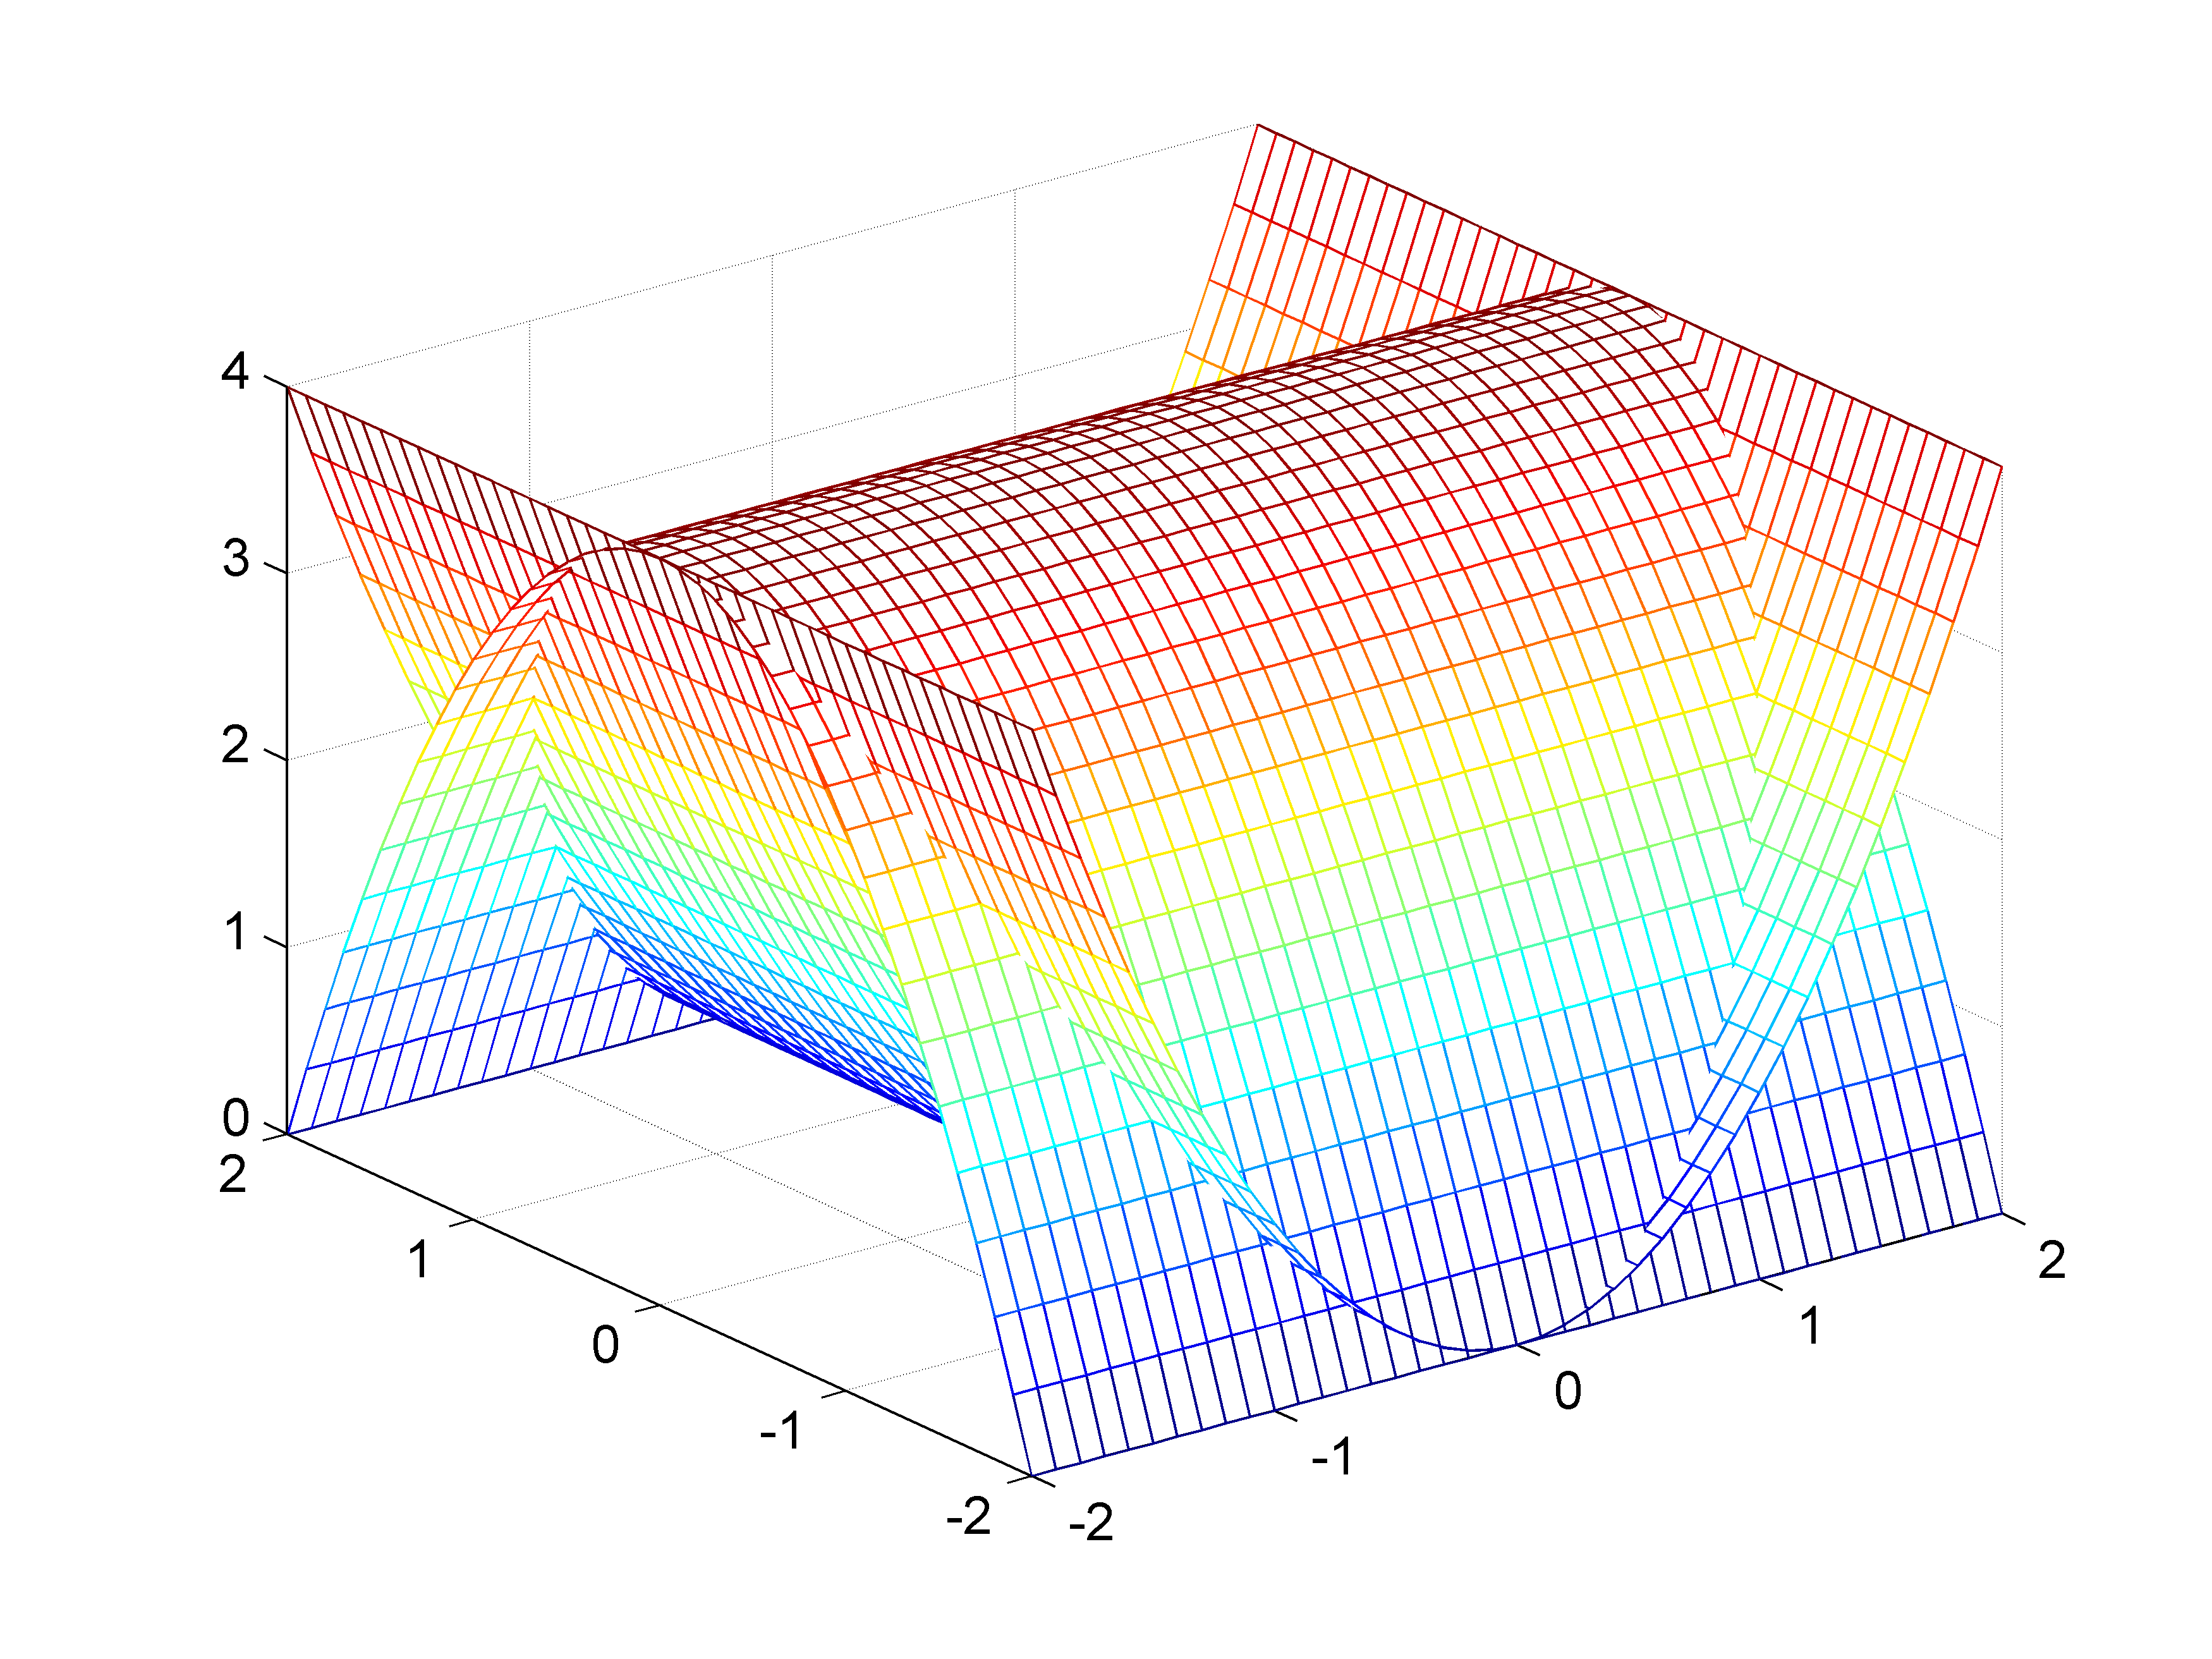
\includegraphics[width=300pt]{./Imagenes/superficies1.png}


Ahora vamos a generar el gráfico de la curva de intersección:
\begin{lstlisting}[language=Matlab]
>> t=0:pi/32:2*pi;
>> u=2*cos(t);
>> v=2*sin(t);
>> w=4*(cos(t)).^2;
>> plot3(u,v,w,'r')
\end{lstlisting}
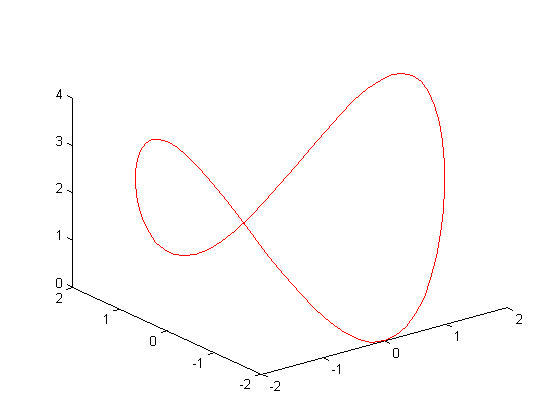
\includegraphics[width=300pt]{./Imagenes/superficies2.png}

Para obtener la proyección de esta curva al plano XY, reemplazar w: 
\begin{lstlisting}[language=Matlab]
>> t=0:pi/32:2*pi;
>> u=2*cos(t);
>> v=2*sin(t);
>> w=0*ones(1,65);
>> plot3(u,v,w,'r')
\end{lstlisting}

\item Las dos superficies $S_{1} : z=x^{2}+y^{2}$, $S_{2} : z=2+y$ determinan una curva. Halle las ecuaciones paramétricas de dicha curva y luego representar. Proyectando la curva al plano XY, esto es, igualando las ecuaciones se obtiene $x^{2} + (y-1/2)^{2} = \dfrac{9}{4}$

Ecuaciones paramétricas de la curva:
$$ x(t) = (3/2)cos(t) $$
$$ y(t) = (3/2)sin t+(1/2) $$
Si reemplazamos $y(t)$ en $z(t)$, se tiene $z(t)=\dfrac{5}{2}+(\dfrac{3}{2})sin(t) $

\begin{lstlisting}[language=Matlab]
>> [x,y]=meshgrid(-2:0.1:2);
>> z=x.^2+y.^2;
>> mesh(x,y,z)
>> hold on
>> z=2+y;
>> mesh(x,y,z)
>> t=0:pi/32:2*pi;
>> u=1.5*cos(t);
>> v=1.5*sin(t)+0.5;
>> w=2.5*ones(1,65)+1.5*sin(t);
>> plot3(u,v,w,'r')
\end{lstlisting}
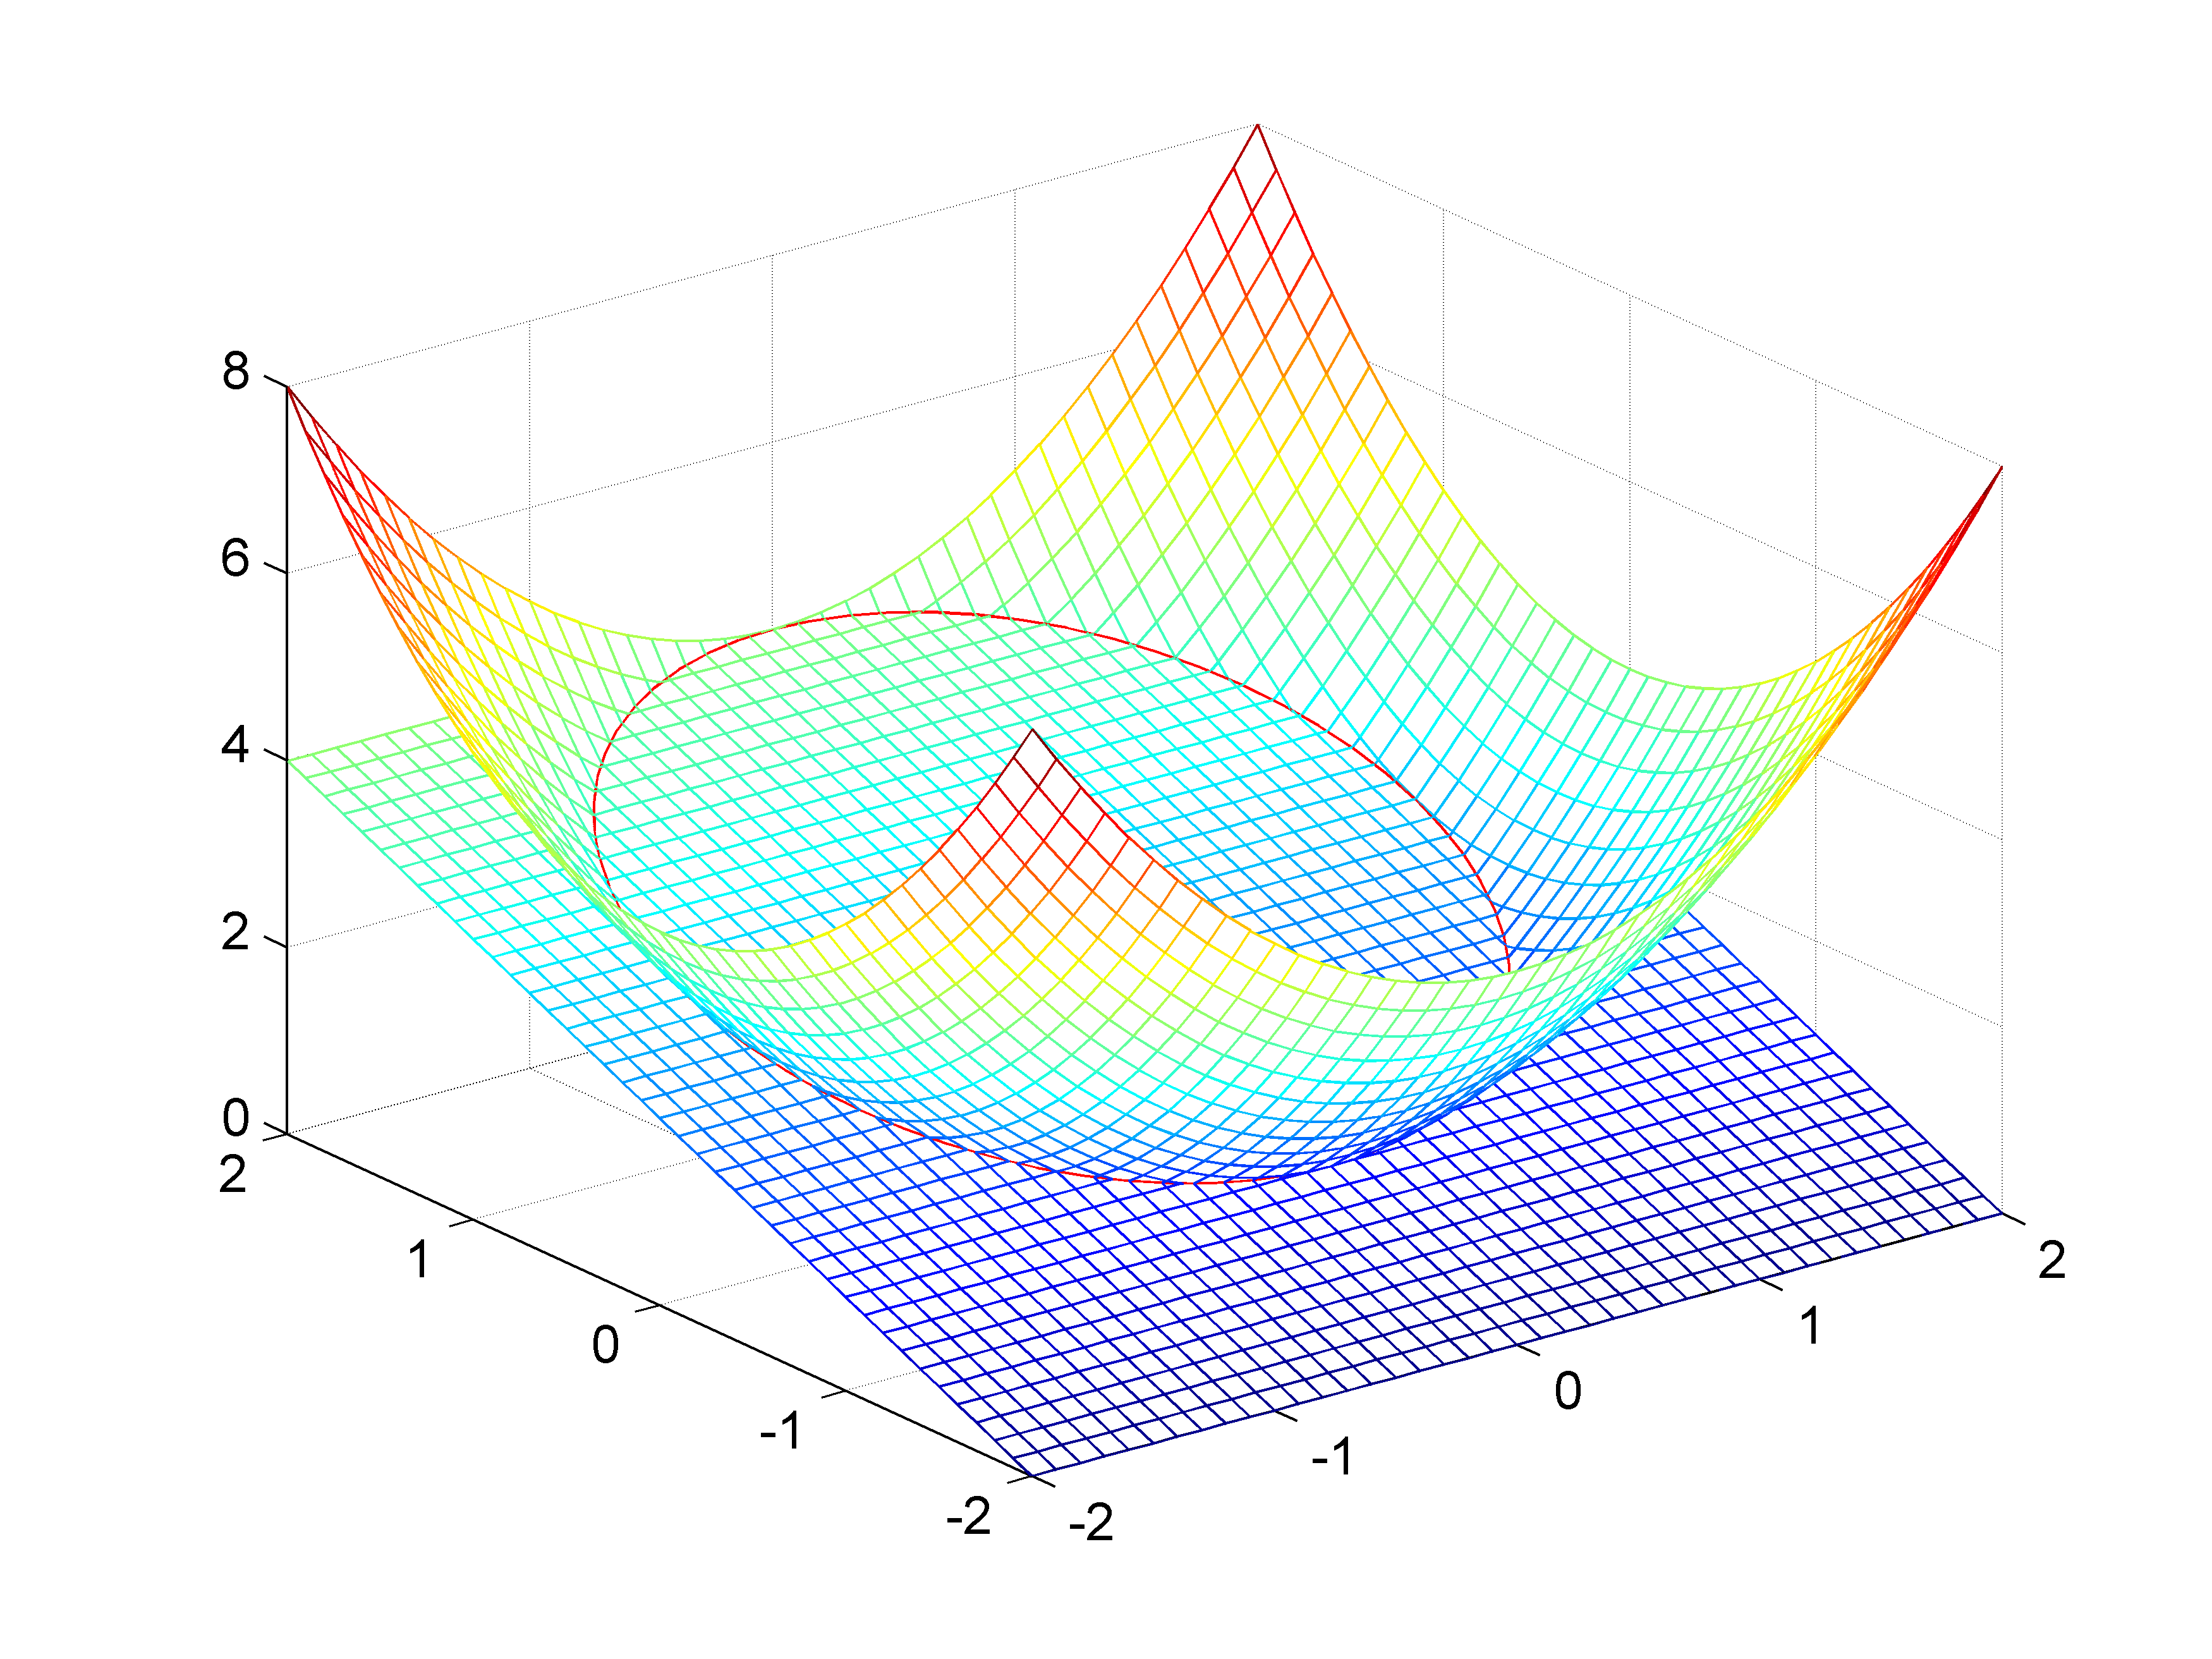
\includegraphics[width=300pt]{./Imagenes/superficies4.png}

\end{enumerate} 

\section{Curvas de nivel}

Sea $S$ una superficie representada por $z=f(x;y)$. La importancia de las curvas de nivel estriba en que trazando un número adecuado de ellas, podemos obtener una buena descripción de la superficie. A continuación se expone un ejemplo de como hallar las curvas de nivel:

\begin{enumerate}
\item Las curvas de nivel de la superficie $S: z = f(x,y) = 4^{2} + y^{2}$ son familias de elipses concentricas en el origen de coordenadas con semiejes  $\sqrt{k}/2$ y  $\sqrt{k}$, con $k>0$. 

$$ 4x^{2}+y^{2} = k \Rightarrow \dfrac{x^{2}}{\frac{k}{4}} + \dfrac{y^{2}}{k} = 1 $$

Gráfica de la superficie y algunas curvas de nivel:
\begin{lstlisting}[language=Matlab]
>> [x,y]=meshgrid(-2:.1:2); 
>> z=4*x.^2+y.^2; 
>> contour(x,y,z,10)
>> contour3(x,y,z,10) 
>> meshc(x,y,z)
\end{lstlisting}
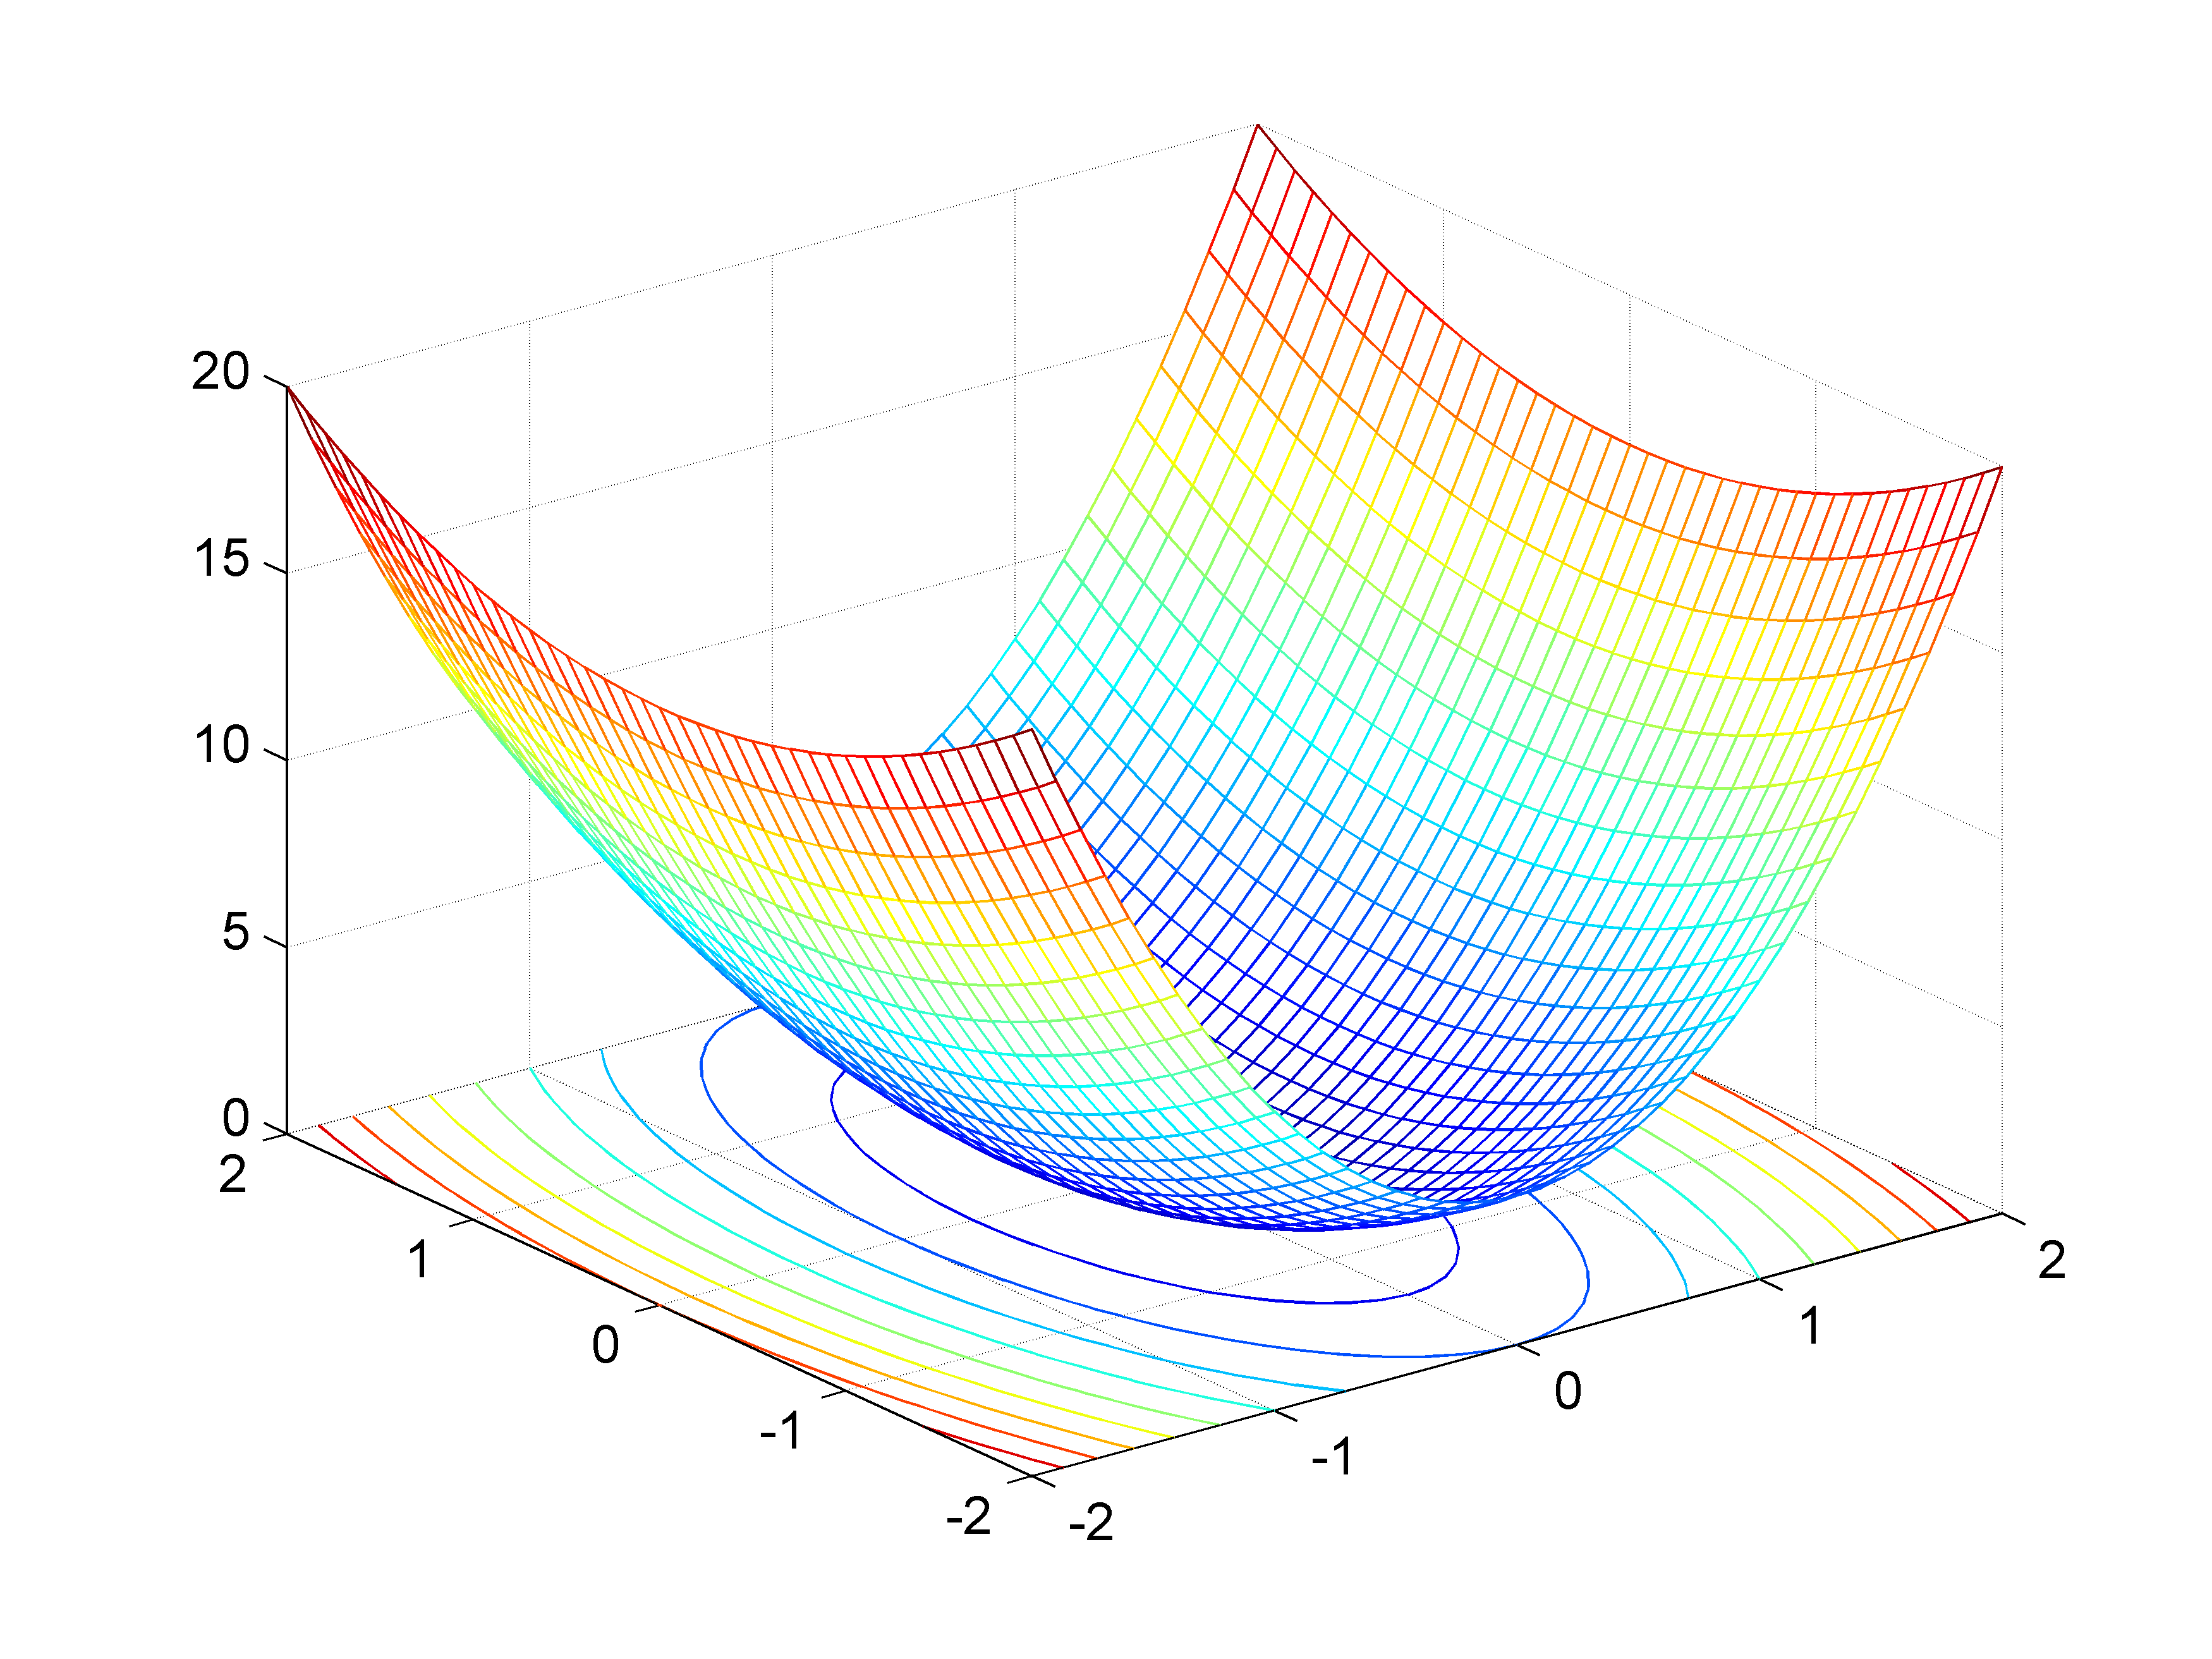
\includegraphics[width=300pt]{./Imagenes/curvanivel1.png}

La superficie y las curvas de nivel están generadas con \textbf{meshc}.
\end{enumerate} 

\section{Superficies de revolución}

Una superficie de revolución es la engendrada por la rotación de una curva plana en torno de 
una recta fija contenida en el plano de la curva. La curva plana se llama \textit{generatriz}, y la recta fija \textit{eje de revolución} o, simplemente eje de la superficie. Cualquier posición de la generatriz se llama \textit{meridiano}, y cada circunferencia descrita por un punto de la generatriz se llama \textit{paralelo} de la superficie.

Para determinar la ecuación de una superficie de revolución, no se pierde generalidad si se toma la generatriz en uno de los planos coordenados y como eje de revolución a uno de los ejes 
coordenados contenidos en ese plano.

Sea G la curva generatriz contenida en el semiplano superior YZ, $G : z = f(y) \geqslant 0 $ y el eje de revolución el eje Z. Sea $P(x;y;z)$, un punto cualquiera de la superficie. El paralelo que pasa por P corta a G en un punto del plano YZ, digamos $Q(0;y^{'};z^{'})$, y su centro $A(0;0;z^{'})$ está sobre el eje de revolución, el eje Z.

Por ser radios del mismo paralelo,$\mid AP \mid$ = $\mid AQ \mid$ entonces
$ z^{'}= \pm \sqrt{x^{2} + y^{2}}$. Además, P y Q están en el mismo plano, entonces $z^{'}=z$. Como $Q \in G : z^{'}=f(y^{'})$.

Reemplazando $y^{'}$, $z^{'}$, en $z^{'} = f(y^{'})$ se obtiene la ecuación de la superficie de revolución $z = f(\sqrt{x^{2} + y^{2}})$.

Representaremos a las superficies de revolución como si fueran superficies paramétricas, 
considerando a \textbf{x} e \textbf{y} como parámetros.

\textbf{Ejemplo}: Sea la curva $C : z = y^{2}$ en el plano YZ. Si el eje de rotación es el eje Z, hallamos la ecuación de la superficie de revolución que genera C.

\textbf{Solución}: En el plano $z=z_{0}$ se encuentra un paralelo, cuyo centro es $A(0;0;z_{0})$. El punto $Q(0;y_{0};z_{0})$ es un punto que resulta de la intersección de C con el plano $z=z_{0}$. Si $P(x;y;z)$ es un punto arbitrario de la superficie que se encuentra en el paralelo entonces $\mid AP \mid$ = $\mid AQ \mid$ y esto implica que $\mid y_{0} \mid = \sqrt{x^{2} + y^{2}}$. Como $Q \in G : z_{0} = y_{0}^{2}$, entonces la ecuación de la superficie es $ S : z = x^{2}+y^{2}$.

\subsection{Superficies de revolución definidas en MATLAB}

Se pueden representar directamente ciertas superficies de revolución conocidas como esferas, 
cilindros, elipsoides, etc.

\subsubsection{Esfera}

Su gráfica se obtiene con el comando \textbf{sphere(n)}, donde \textbf{n} es el número de puntos en los que queda dividido tanto el ecuador de la esfera como el meridiano principal. A raíz de esa división se representa la esfera con \textbf{n} paralelos y \textbf{n} meridianos. Con \textbf{sphere(20)} se obtiene la esfera con 20 paralelas y 20 meridianos.

\begin{lstlisting}[language=Matlab]
>> sphere(20)
\end{lstlisting}
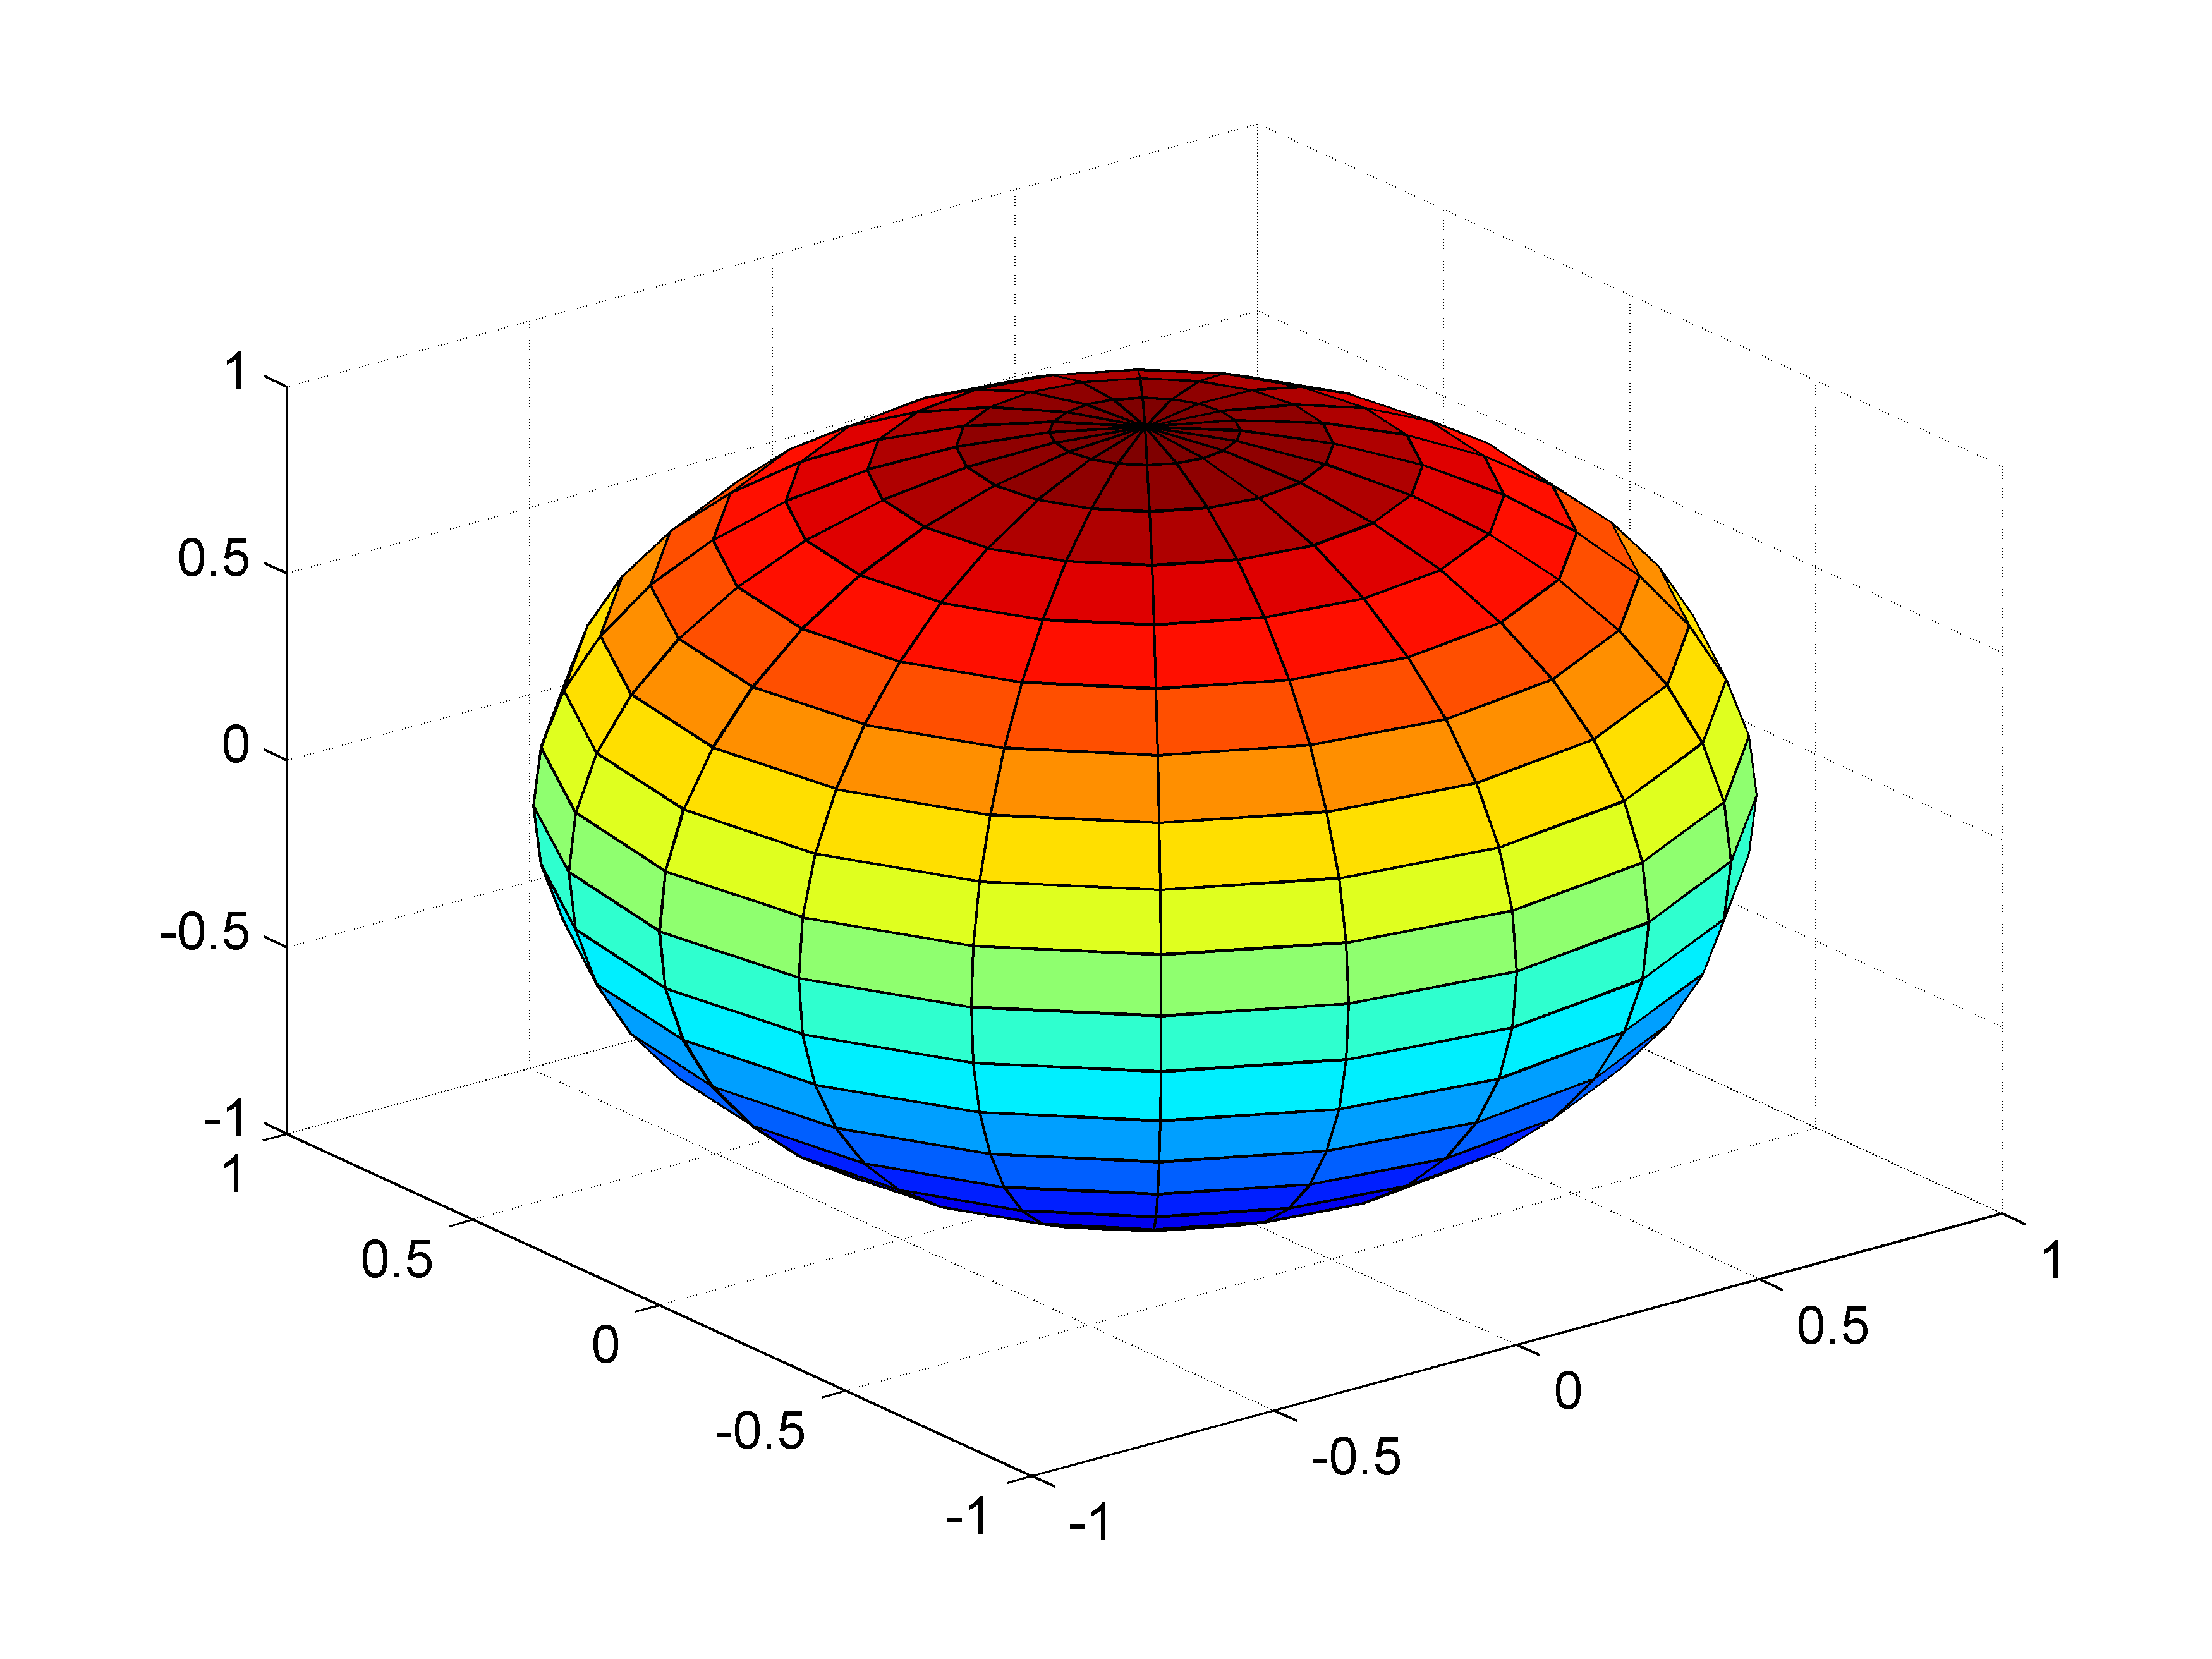
\includegraphics[width=200pt]{./Imagenes/esfera1.png}

Vectores normales a una esfera:
\begin{lstlisting}[language=Matlab]
>> [x,y,z]=sphere(20); 
>> surfnorm(x,y,z)
\end{lstlisting}
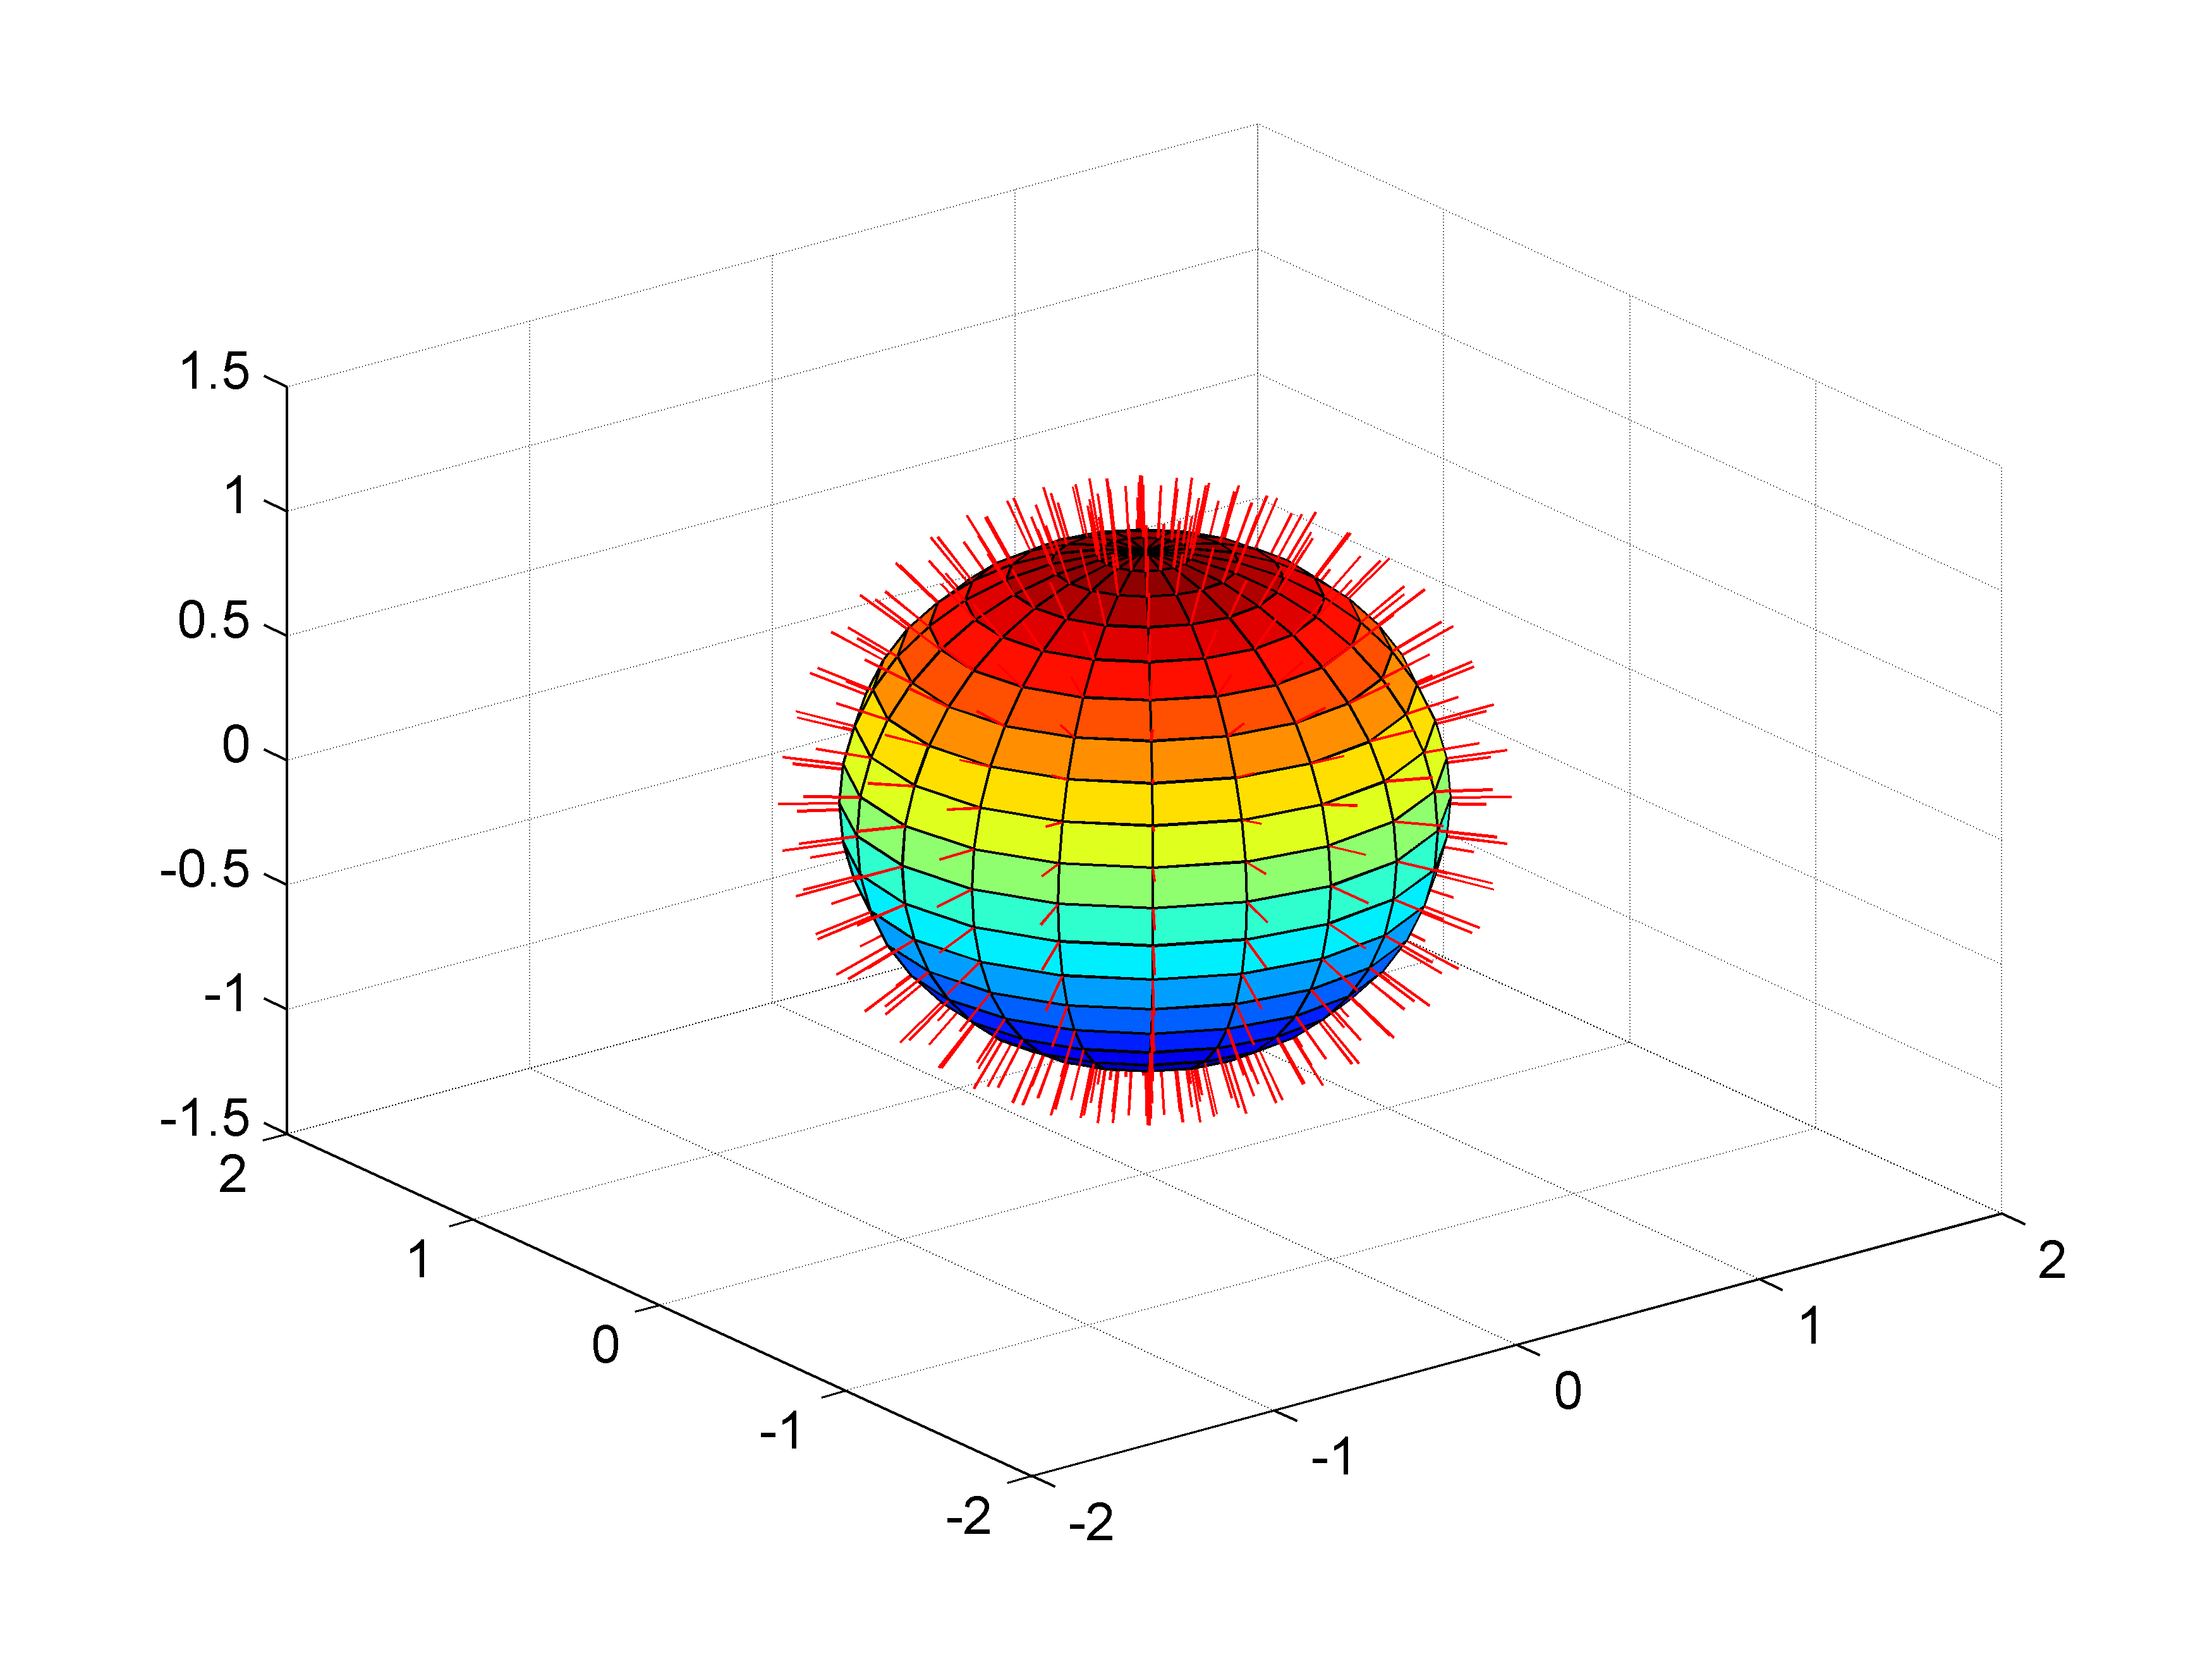
\includegraphics[width=300pt]{./Imagenes/esfera2.png}

\subsubsection{Cilindro}

Se representa mediante el comando \textbf{cylinder}. Este comando \textbf{cylinder(R, n)} genera automáticamente un cilindro de revolución de radio R y n segmentos generatrices. En este caso, la circunferencia de la base del cilindro es dividido en n puntos, por donde pasan dichas generatrices paralelas al eje del cilindro.
\begin{lstlisting}[language=Matlab]
>> cylinder(10,90)
\end{lstlisting}
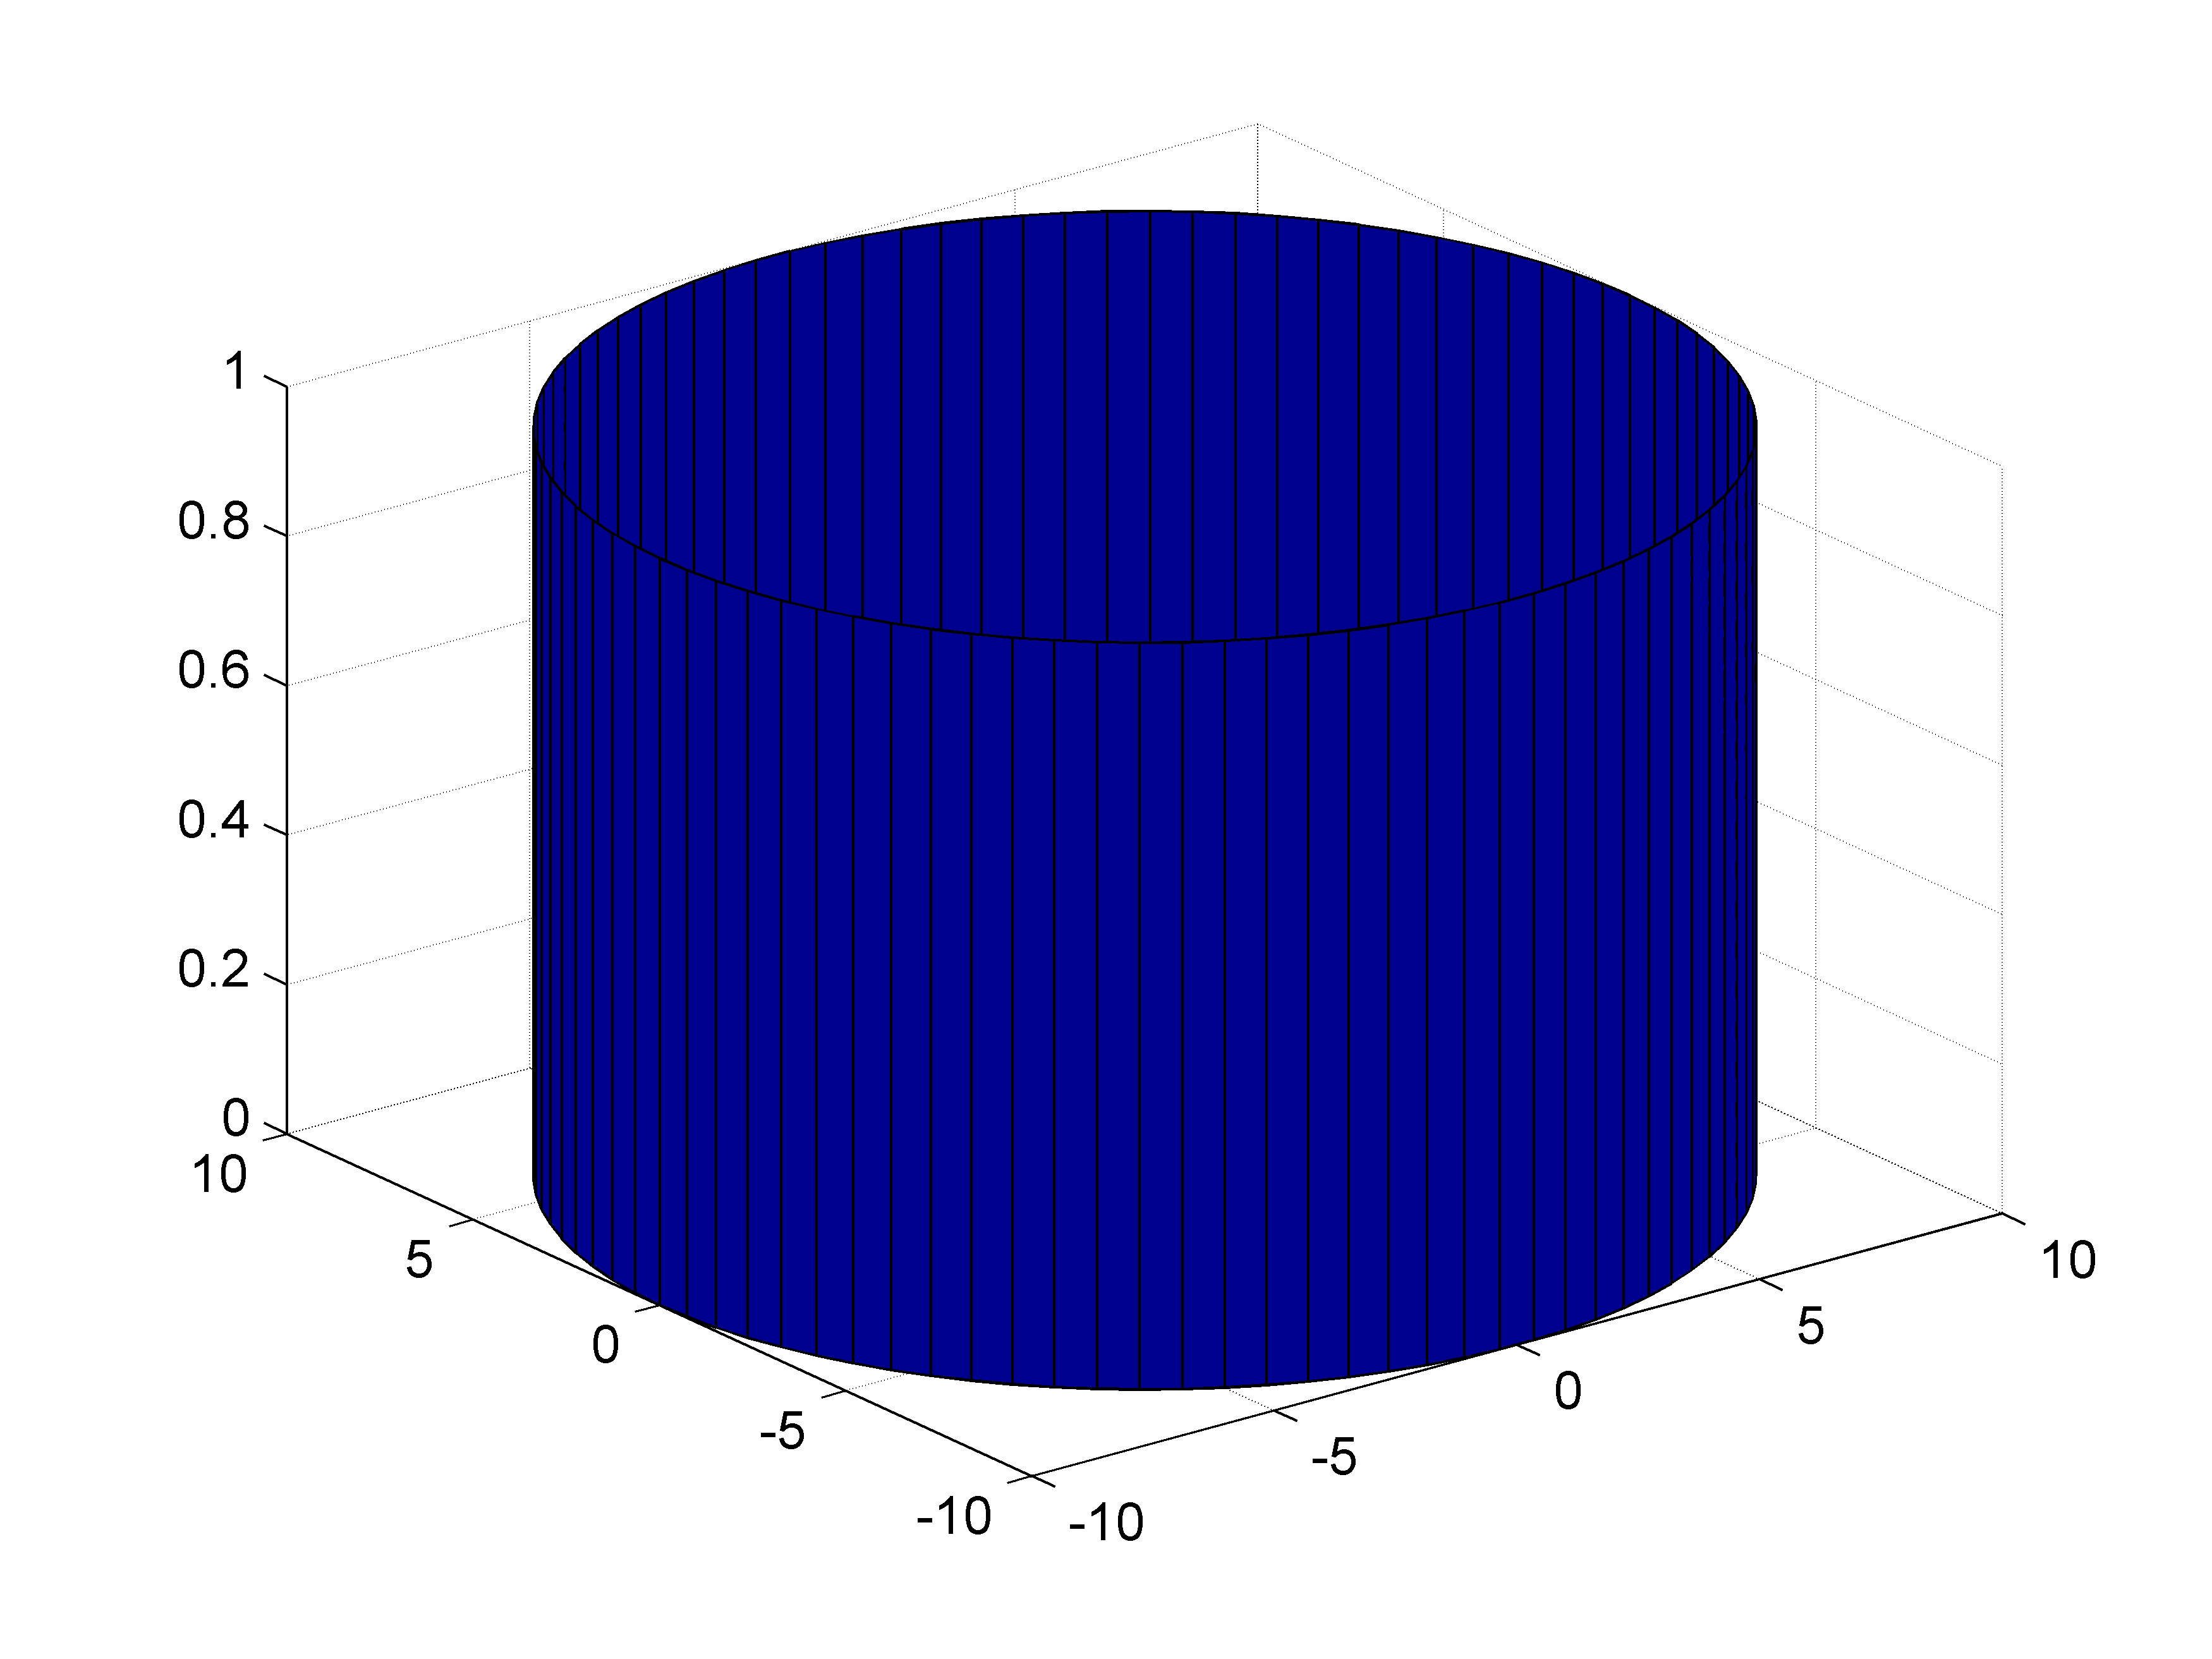
\includegraphics[width=300pt]{./Imagenes/cilindro.png}


\section{Superficies paramétricas}

Una superficie $S$ puede ser representada por una función vectorial $r(u,v) = (x, y, z)$, donde $(u,v) \in D$ en el plano. Las funciones x, y, z dependen de los parámetros u y v. A las ecuaciones:
$$x=x(u,v)$$
$$y=y(u,v)$$
$$z=z(u,v)$$
se denomina ecuaciones paramétricas de $S$.

\textbf{Definición}: Un subconjunto $S$ de $\Re^{3}$ se denomina una superficie regular si para cada p en S existe una vecindad $ V \subset \Re^{3} $ de p, un abierto $ U \subset \Re^{2} $ y una bisección $\varphi : U \longrightarrow V \cap S$ con algunas propiedades que no vamos a ver en este curso. Vamos a ver un ejemplo de como representar una superficie según sus ecuaciones paramétricas.

\begin{enumerate}

\item Superficie de revolución con perfil la curva definida por $r= \sqrt{t}$ , $t \in [0,2]$
\begin{lstlisting}[language=Matlab]
>> t=linspace(0,2,20); 
>> r=sqrt(t); 
>> cylinder(r) 
>> xlabel('t');ylabel('r(t)');zlabel('z(t,r)')
\end{lstlisting}
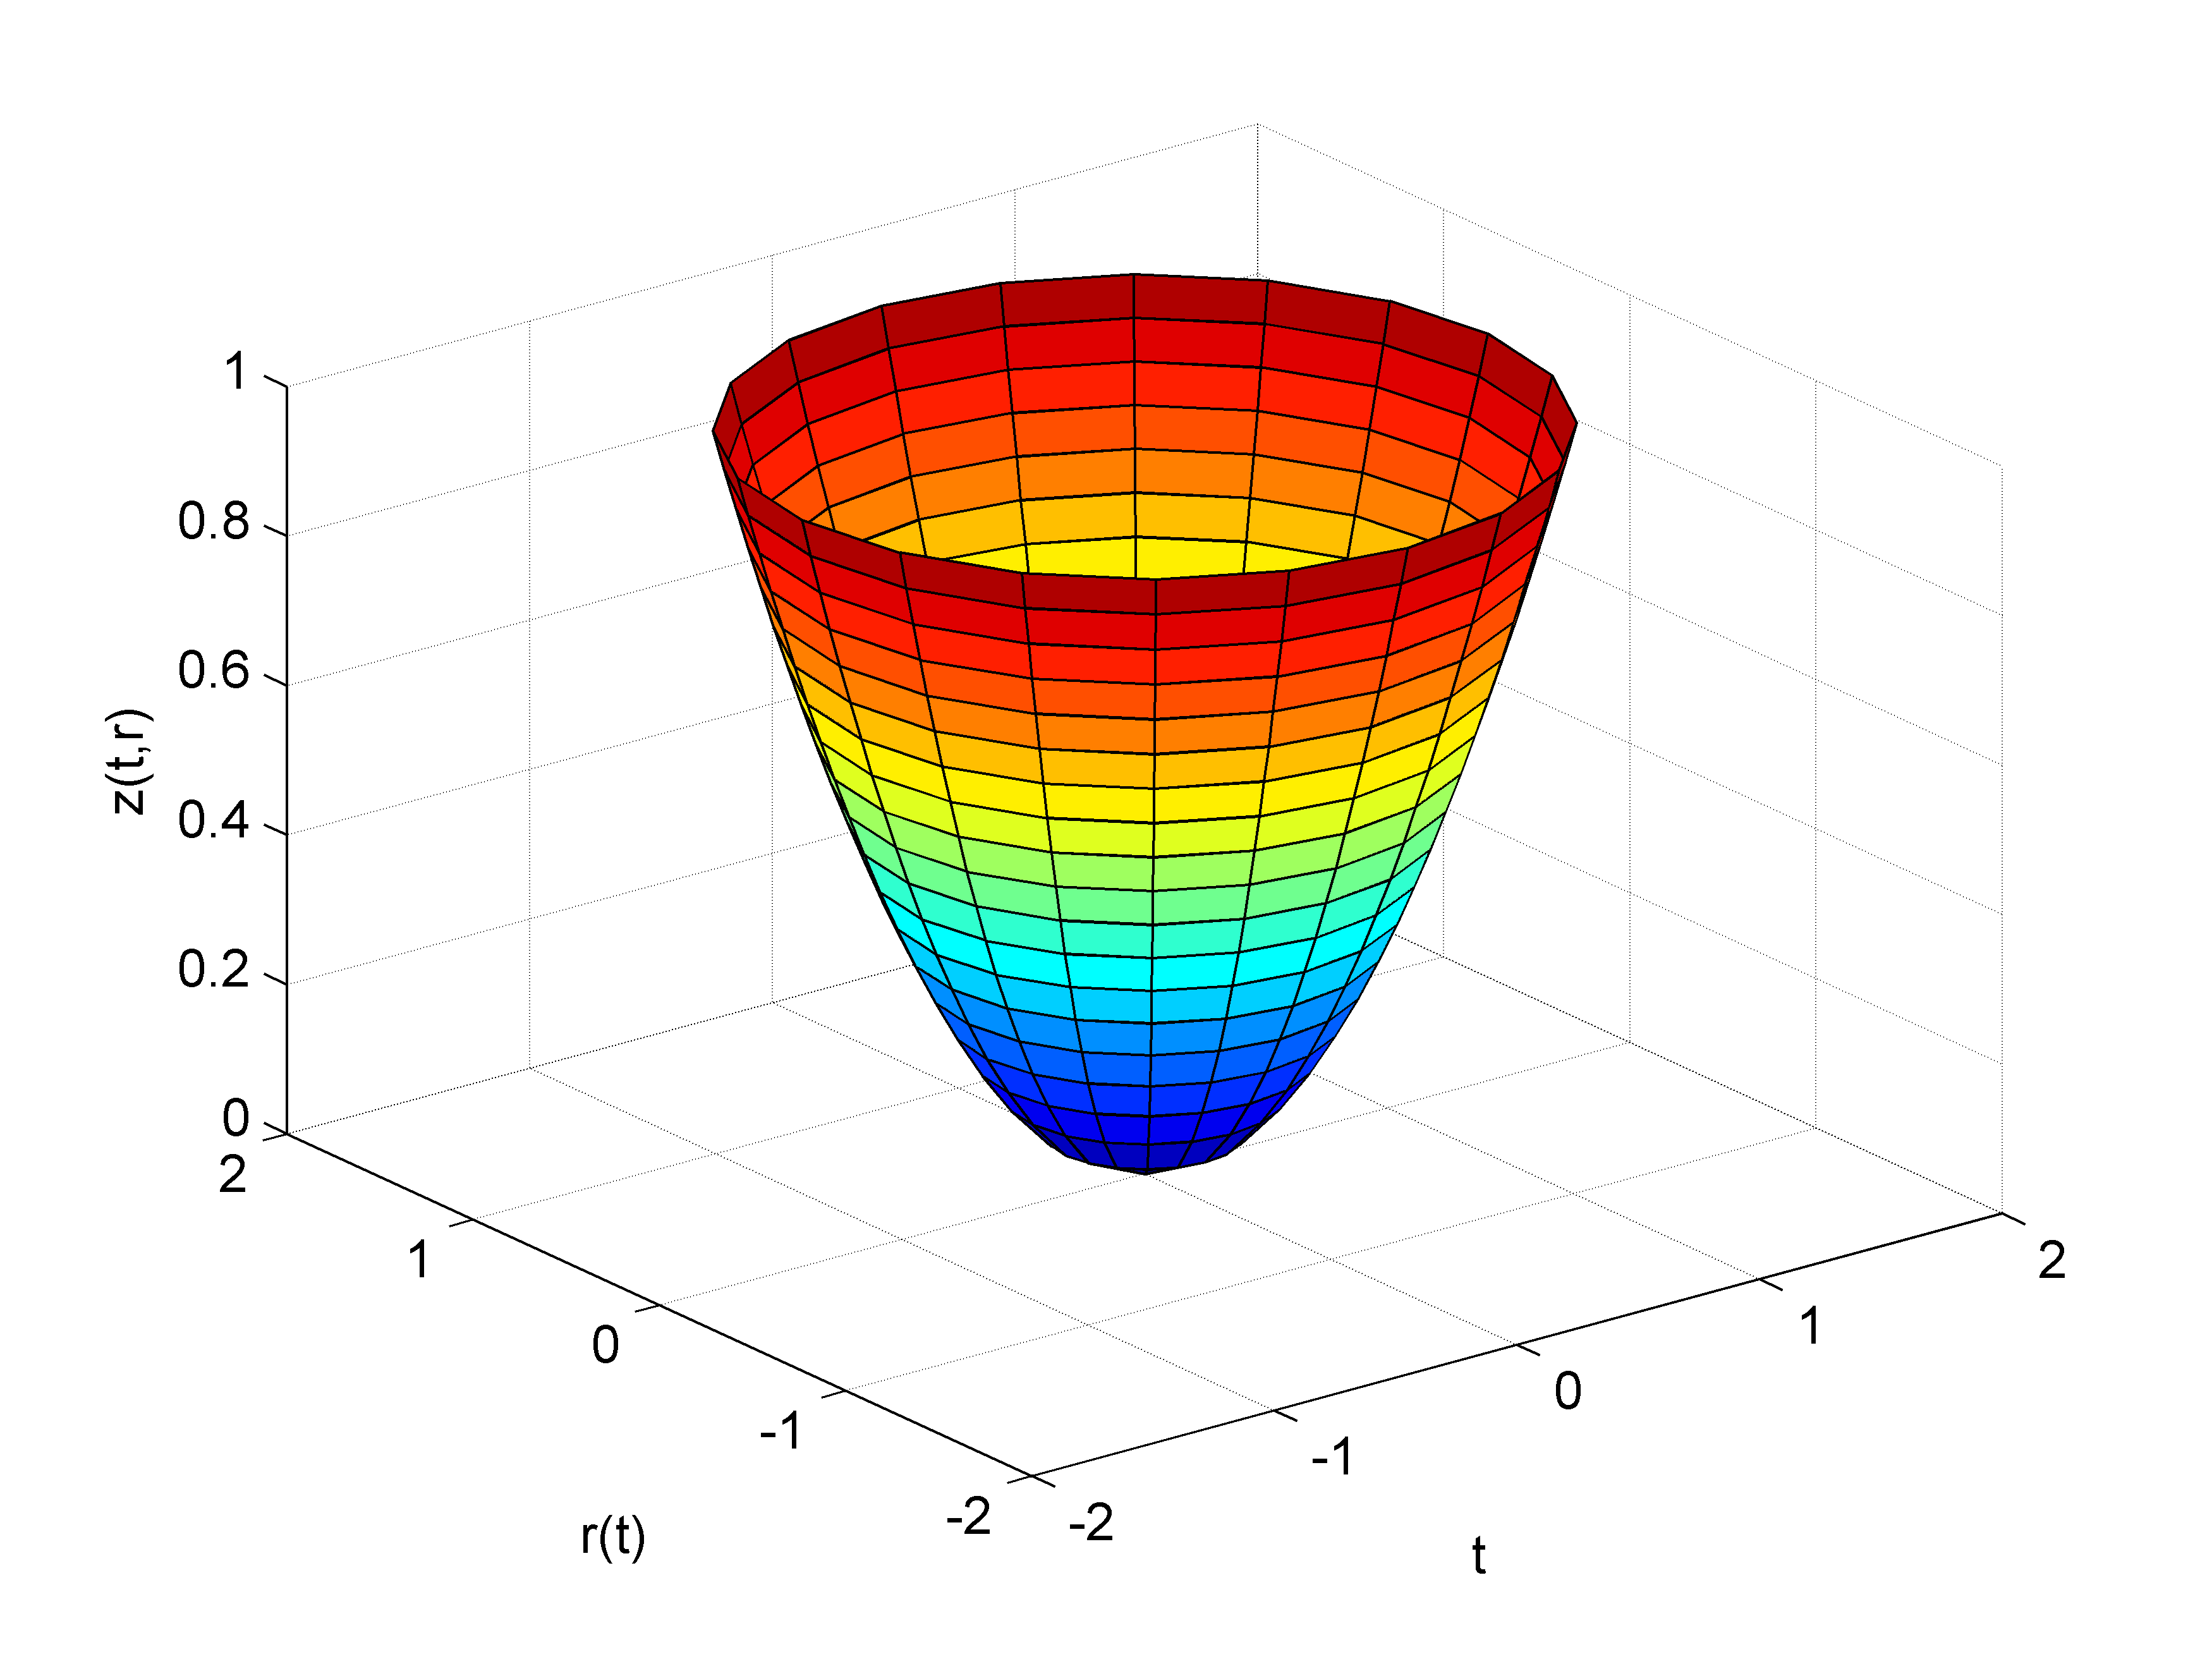
\includegraphics[width=300pt]{./Imagenes/supfparam1.png}


\item Superficie de revolución de perfil $2 + cos(t)$
\begin{lstlisting}[language=Matlab]
>> t = 0:pi/10:2*pi; 
>> [X,Y,Z] = cylinder(2+cos(t)); 
>> surf(X,Y,Z) 
>> axis square 
>> xlabel('x');ylabel('y');zlabel('z')
\end{lstlisting}
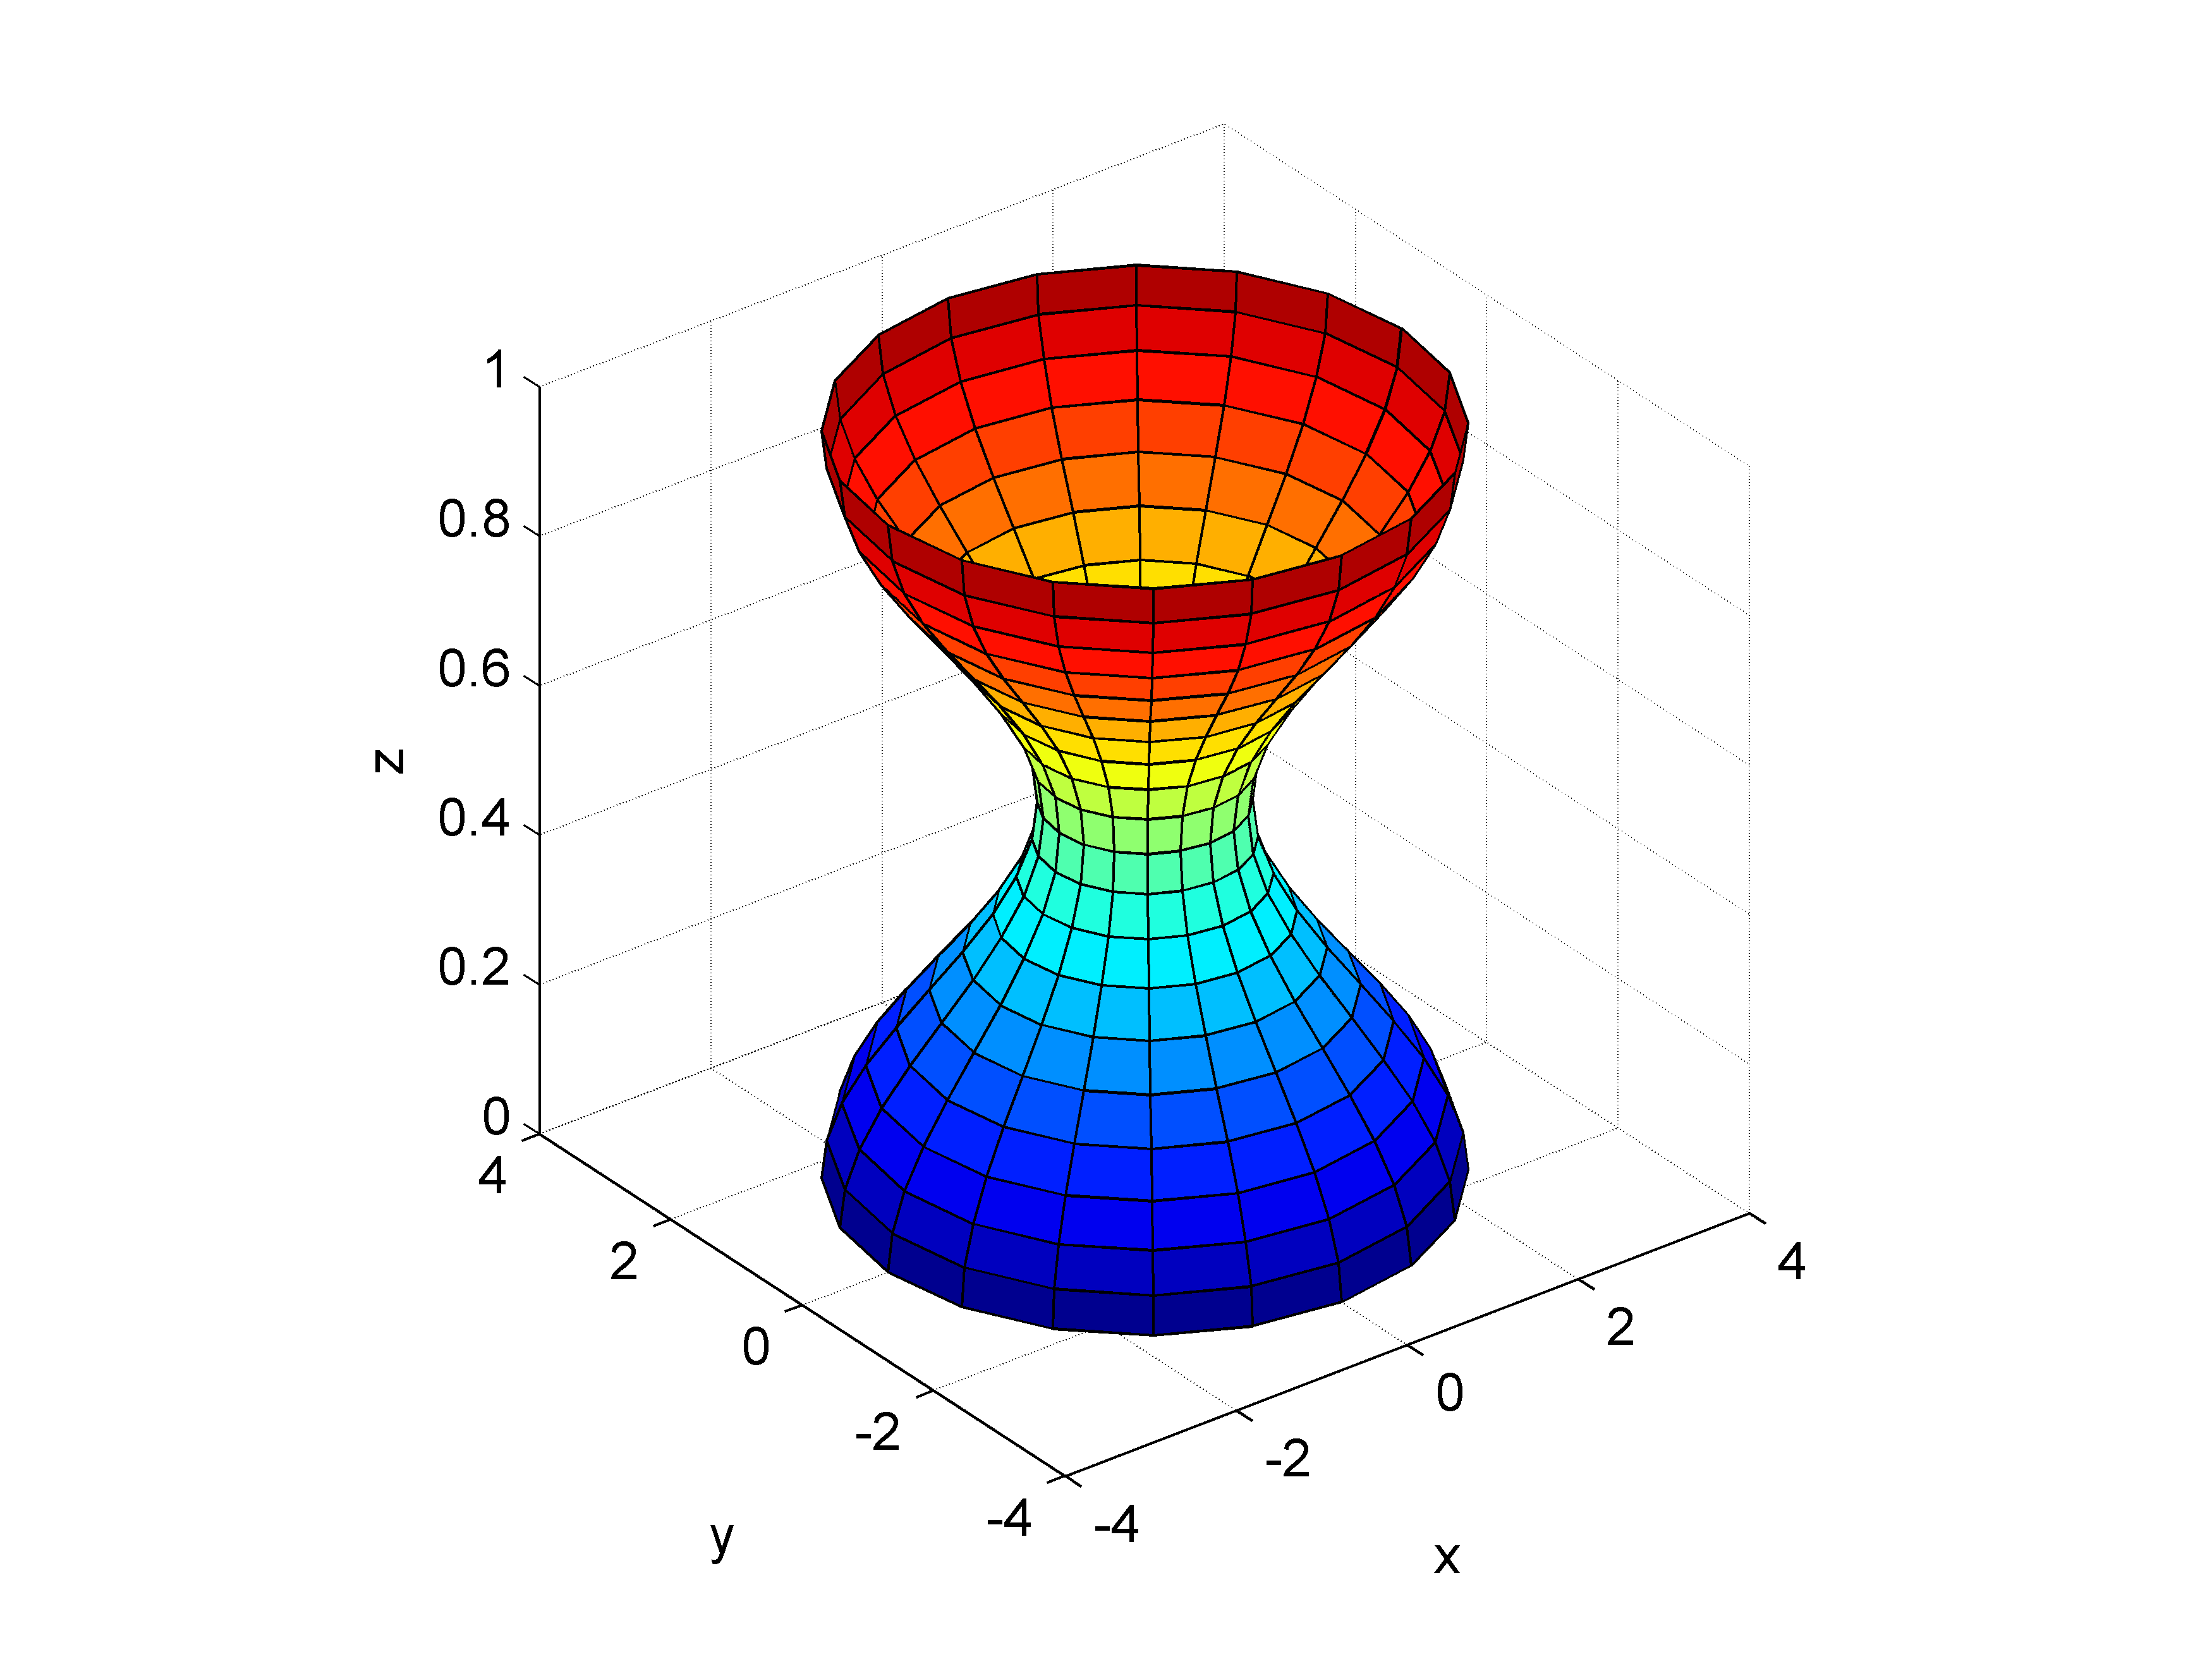
\includegraphics[width=300pt]{./Imagenes/supfparam2.png}

\item Cilindro como superficie de revolución
\begin{lstlisting}[language=Matlab]
>> r=(0:0.1:2*pi)'; 
>> t=-pi:0.1:2*pi; 
>> X=cos(r)*sin(t); 
>> Y=sin(r)*sin(t); 
>> Z=ones(1,size(r))'*t; 
>> surf(X,Y,Z) 
>> axis square
\end{lstlisting}
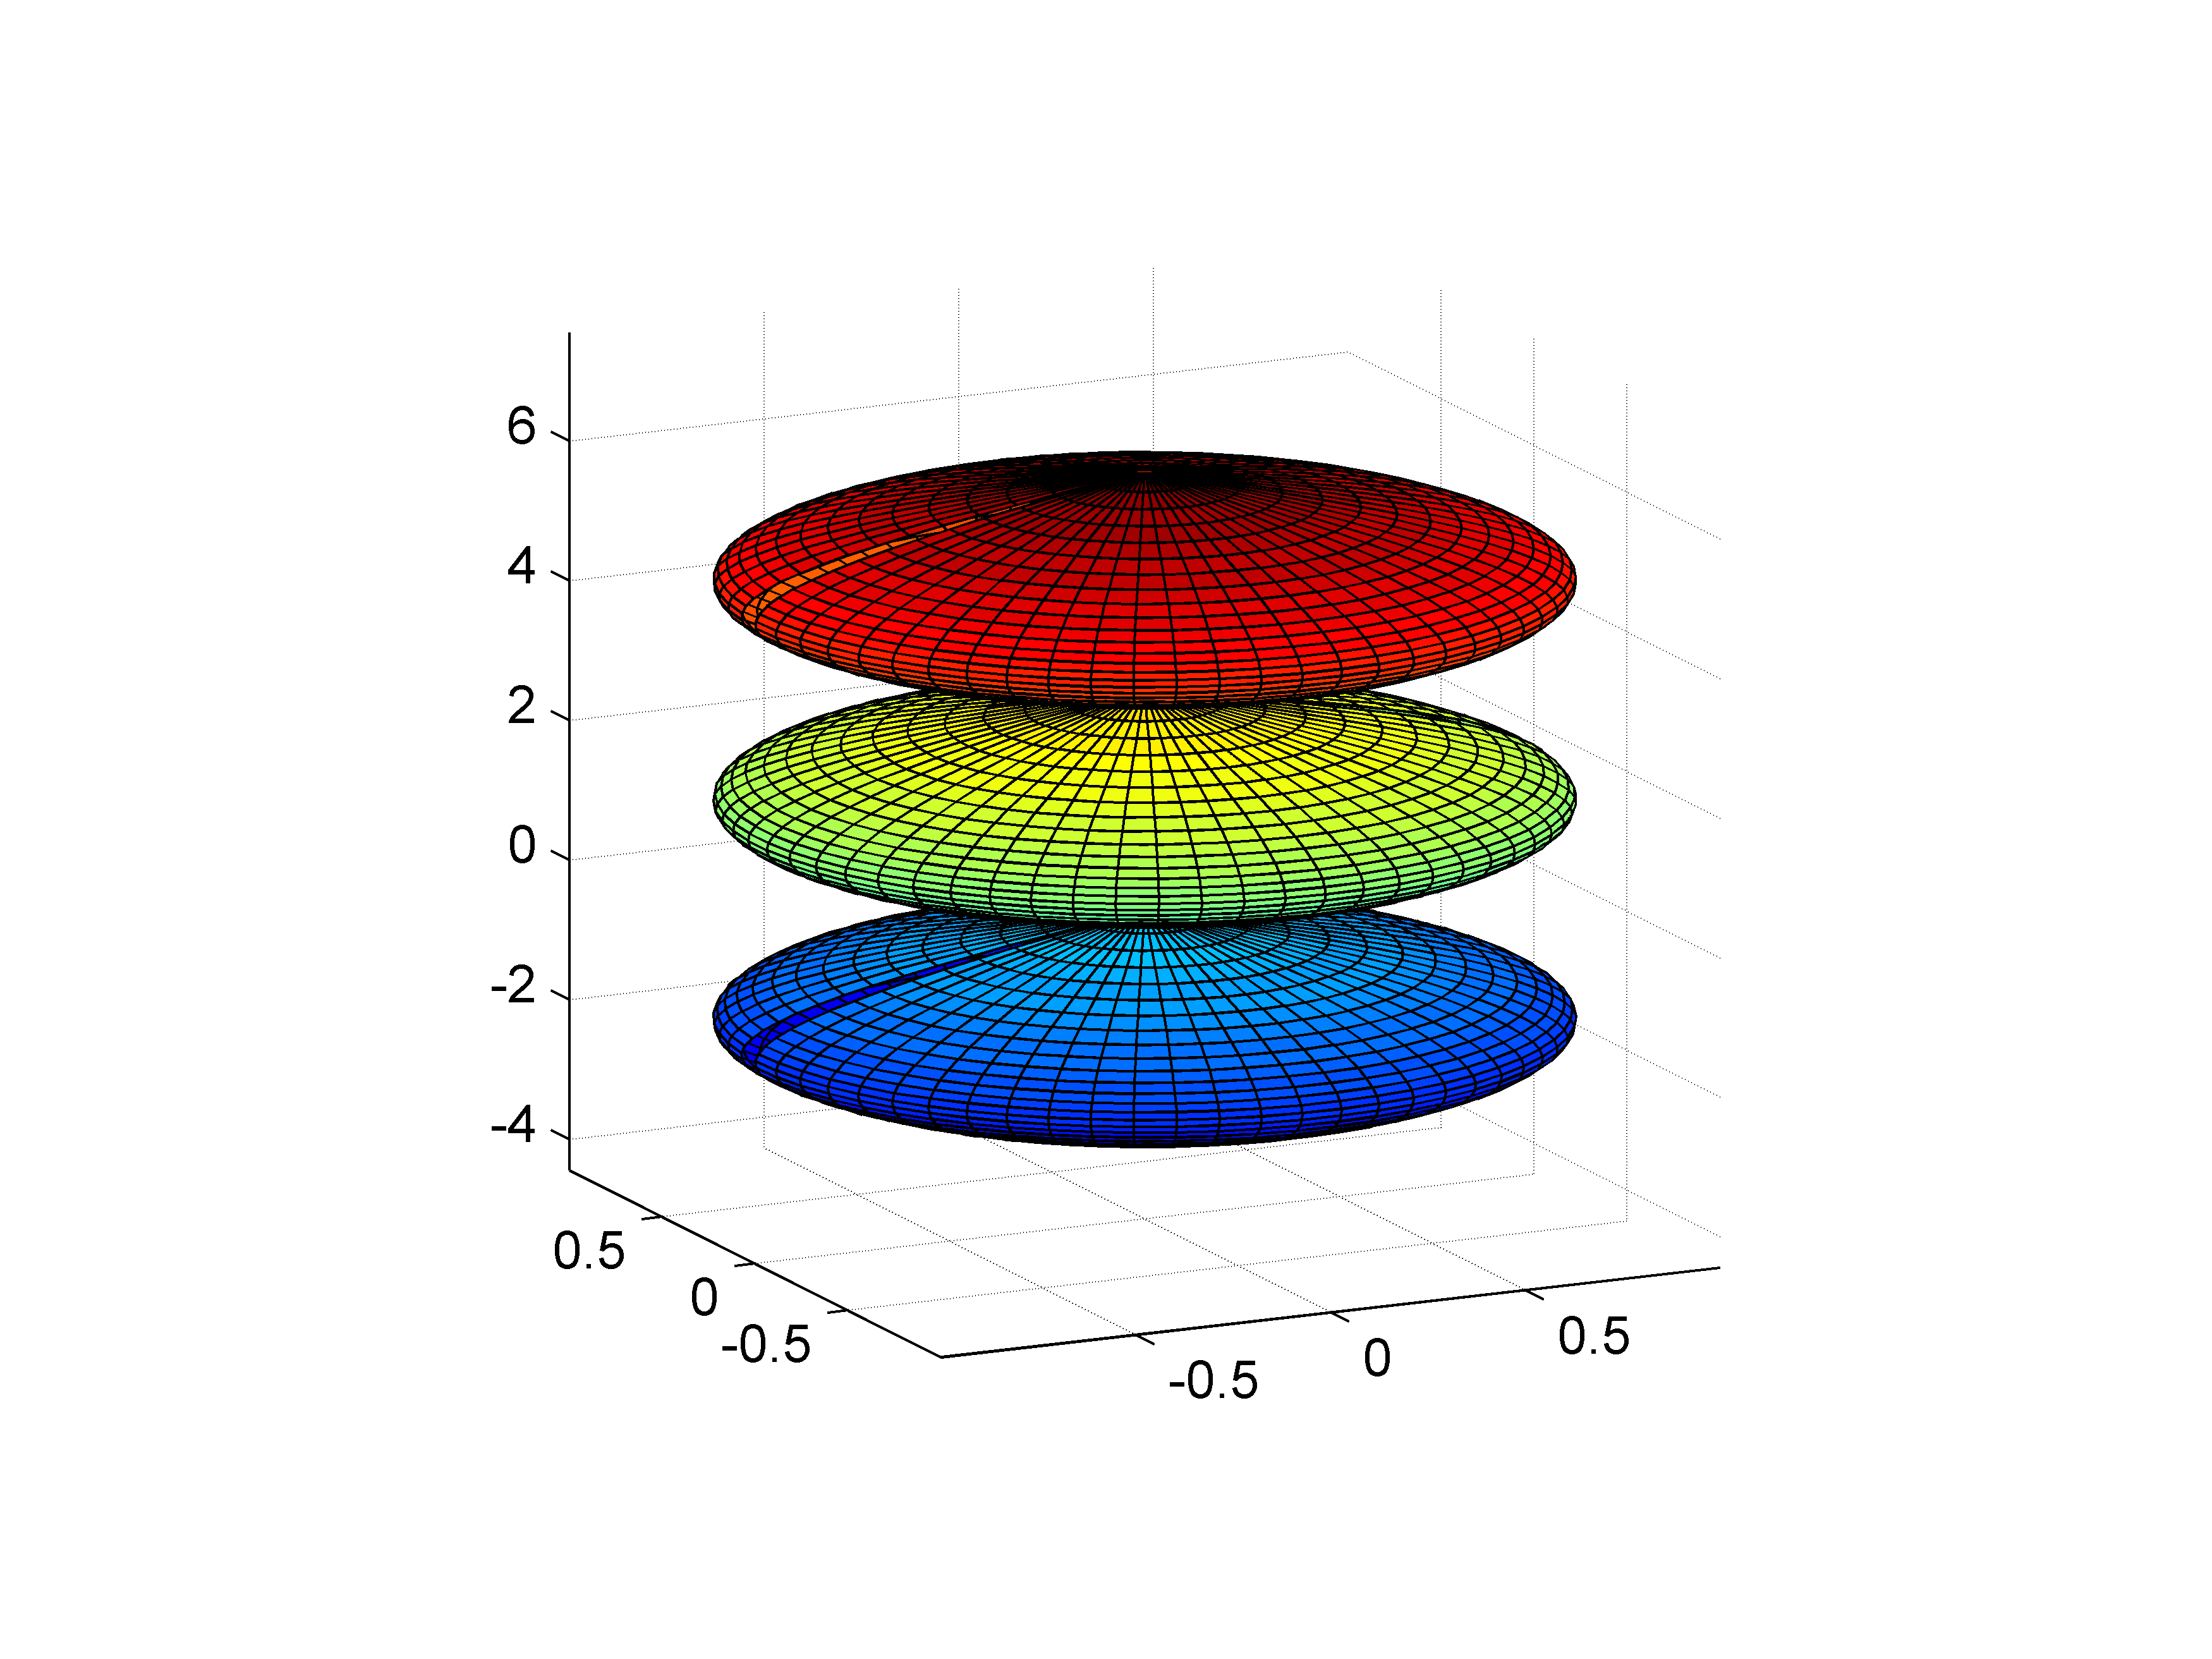
\includegraphics[width=300pt]{./Imagenes/cilindsupf.png}

\item Toroide: Considere en $\Re^{3}$ la circunferencia $C={(x,y,z):(y-2)^{2}+z^{2}=1, x=0}$. 
Al rotar C alrededor del eje Z se obtiene el toro. Una parametrización para esta superficie está dada por $\varphi(u,v) = (cos u(2+cos v),sin u(2+cos v),sin v), 0 \leq u \leq 2\pi ,0 \lq v \leq 2\pi$. 
La gráfica del toro se obtiene con la secuencia de comandos. 

\begin{lstlisting}[language=Matlab]
>> u=linspace(0,2*pi,41); v=u; 
>> [U,V]=meshgrid(u,v); 
>> X=cos(U).*(2+cos(V)); 
>> Y=sin(U).*(2+cos(V)); 
>> Z=sin(V); 
>> surf(X,Y,Z) 
>> axis([-3 3 -3 3 -1 1])
\end{lstlisting}
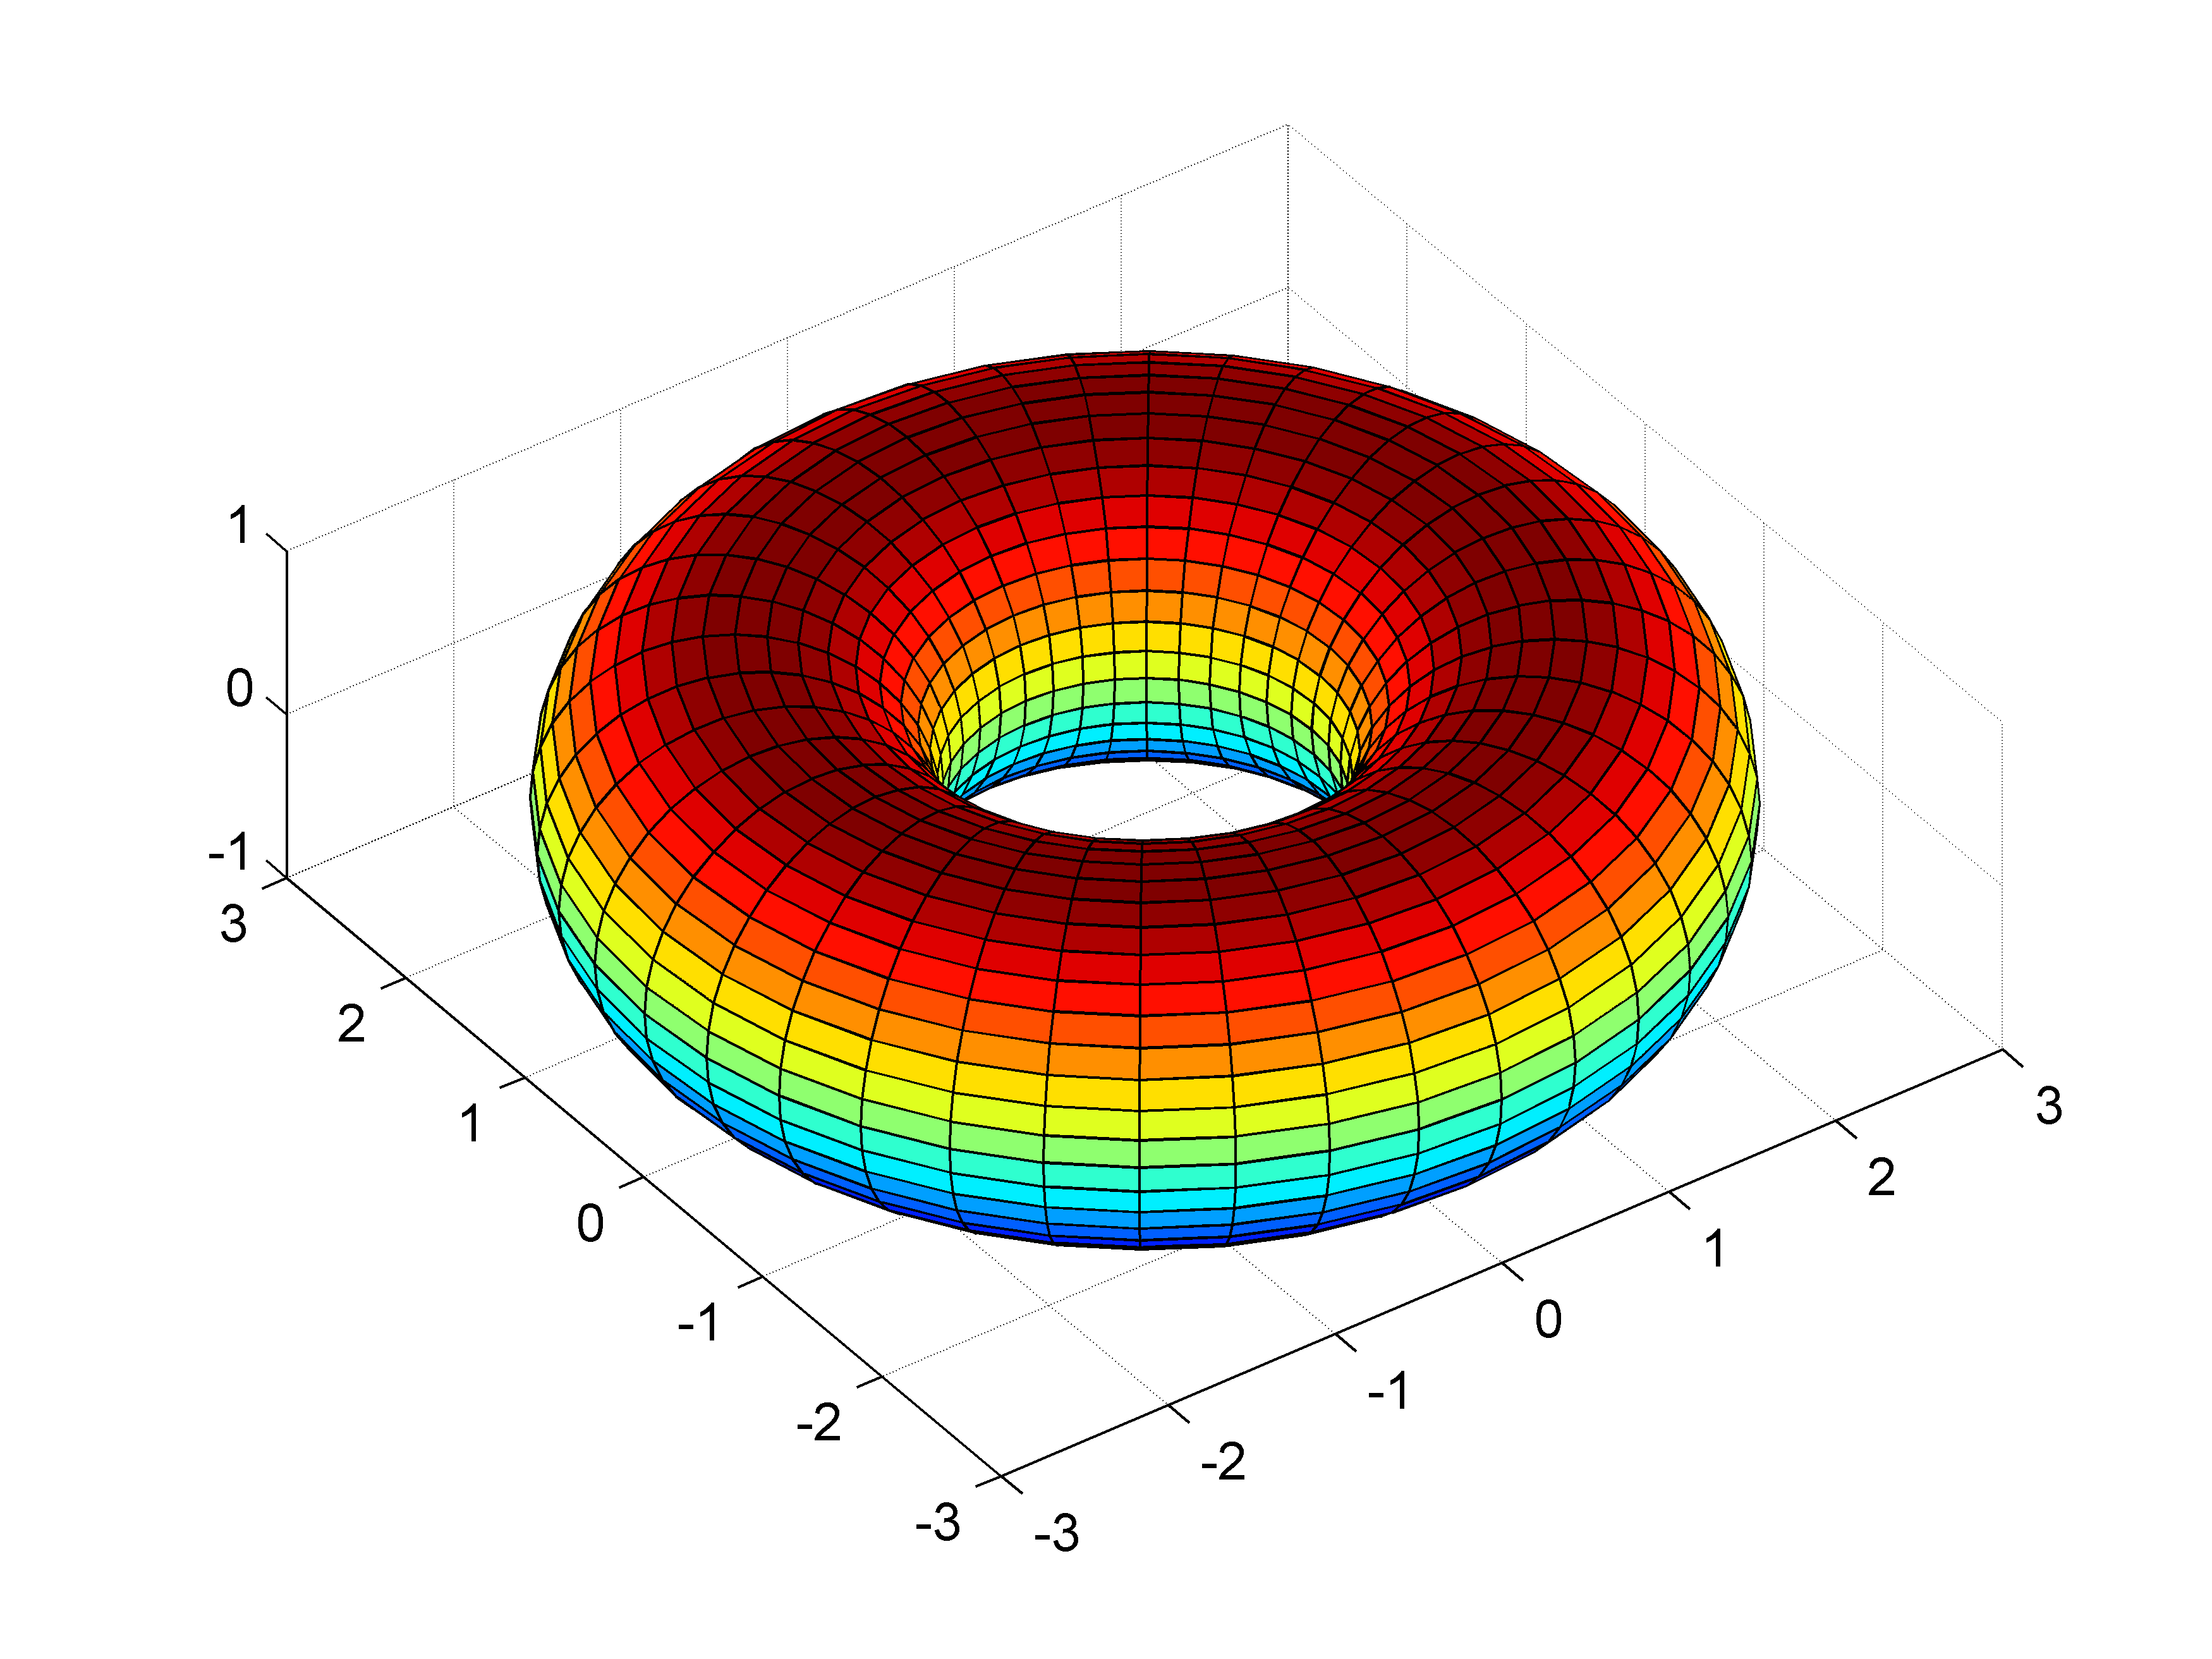
\includegraphics[width=300pt]{./Imagenes/toroide.png}


\item Superficie "Tobogán", variación a la del toro. 

\begin{lstlisting}[language=Matlab]
>> u=(0:pi/8:4*pi)'; 
>> v=0:pi/16:2*pi;
>> X=cos(u)*(2+sin(v)); 
>> Y=sin(u)*(2+sin(v)); 
>> Z=u*ones(size(v))+ones(size(u))*cos(v); 
>> mesh(X,Y,Z)%surfl(X,Y,Z)%surf(X,Y,Z) 
>> axis([-4 4 -4 4 0 10]) 
\end{lstlisting}
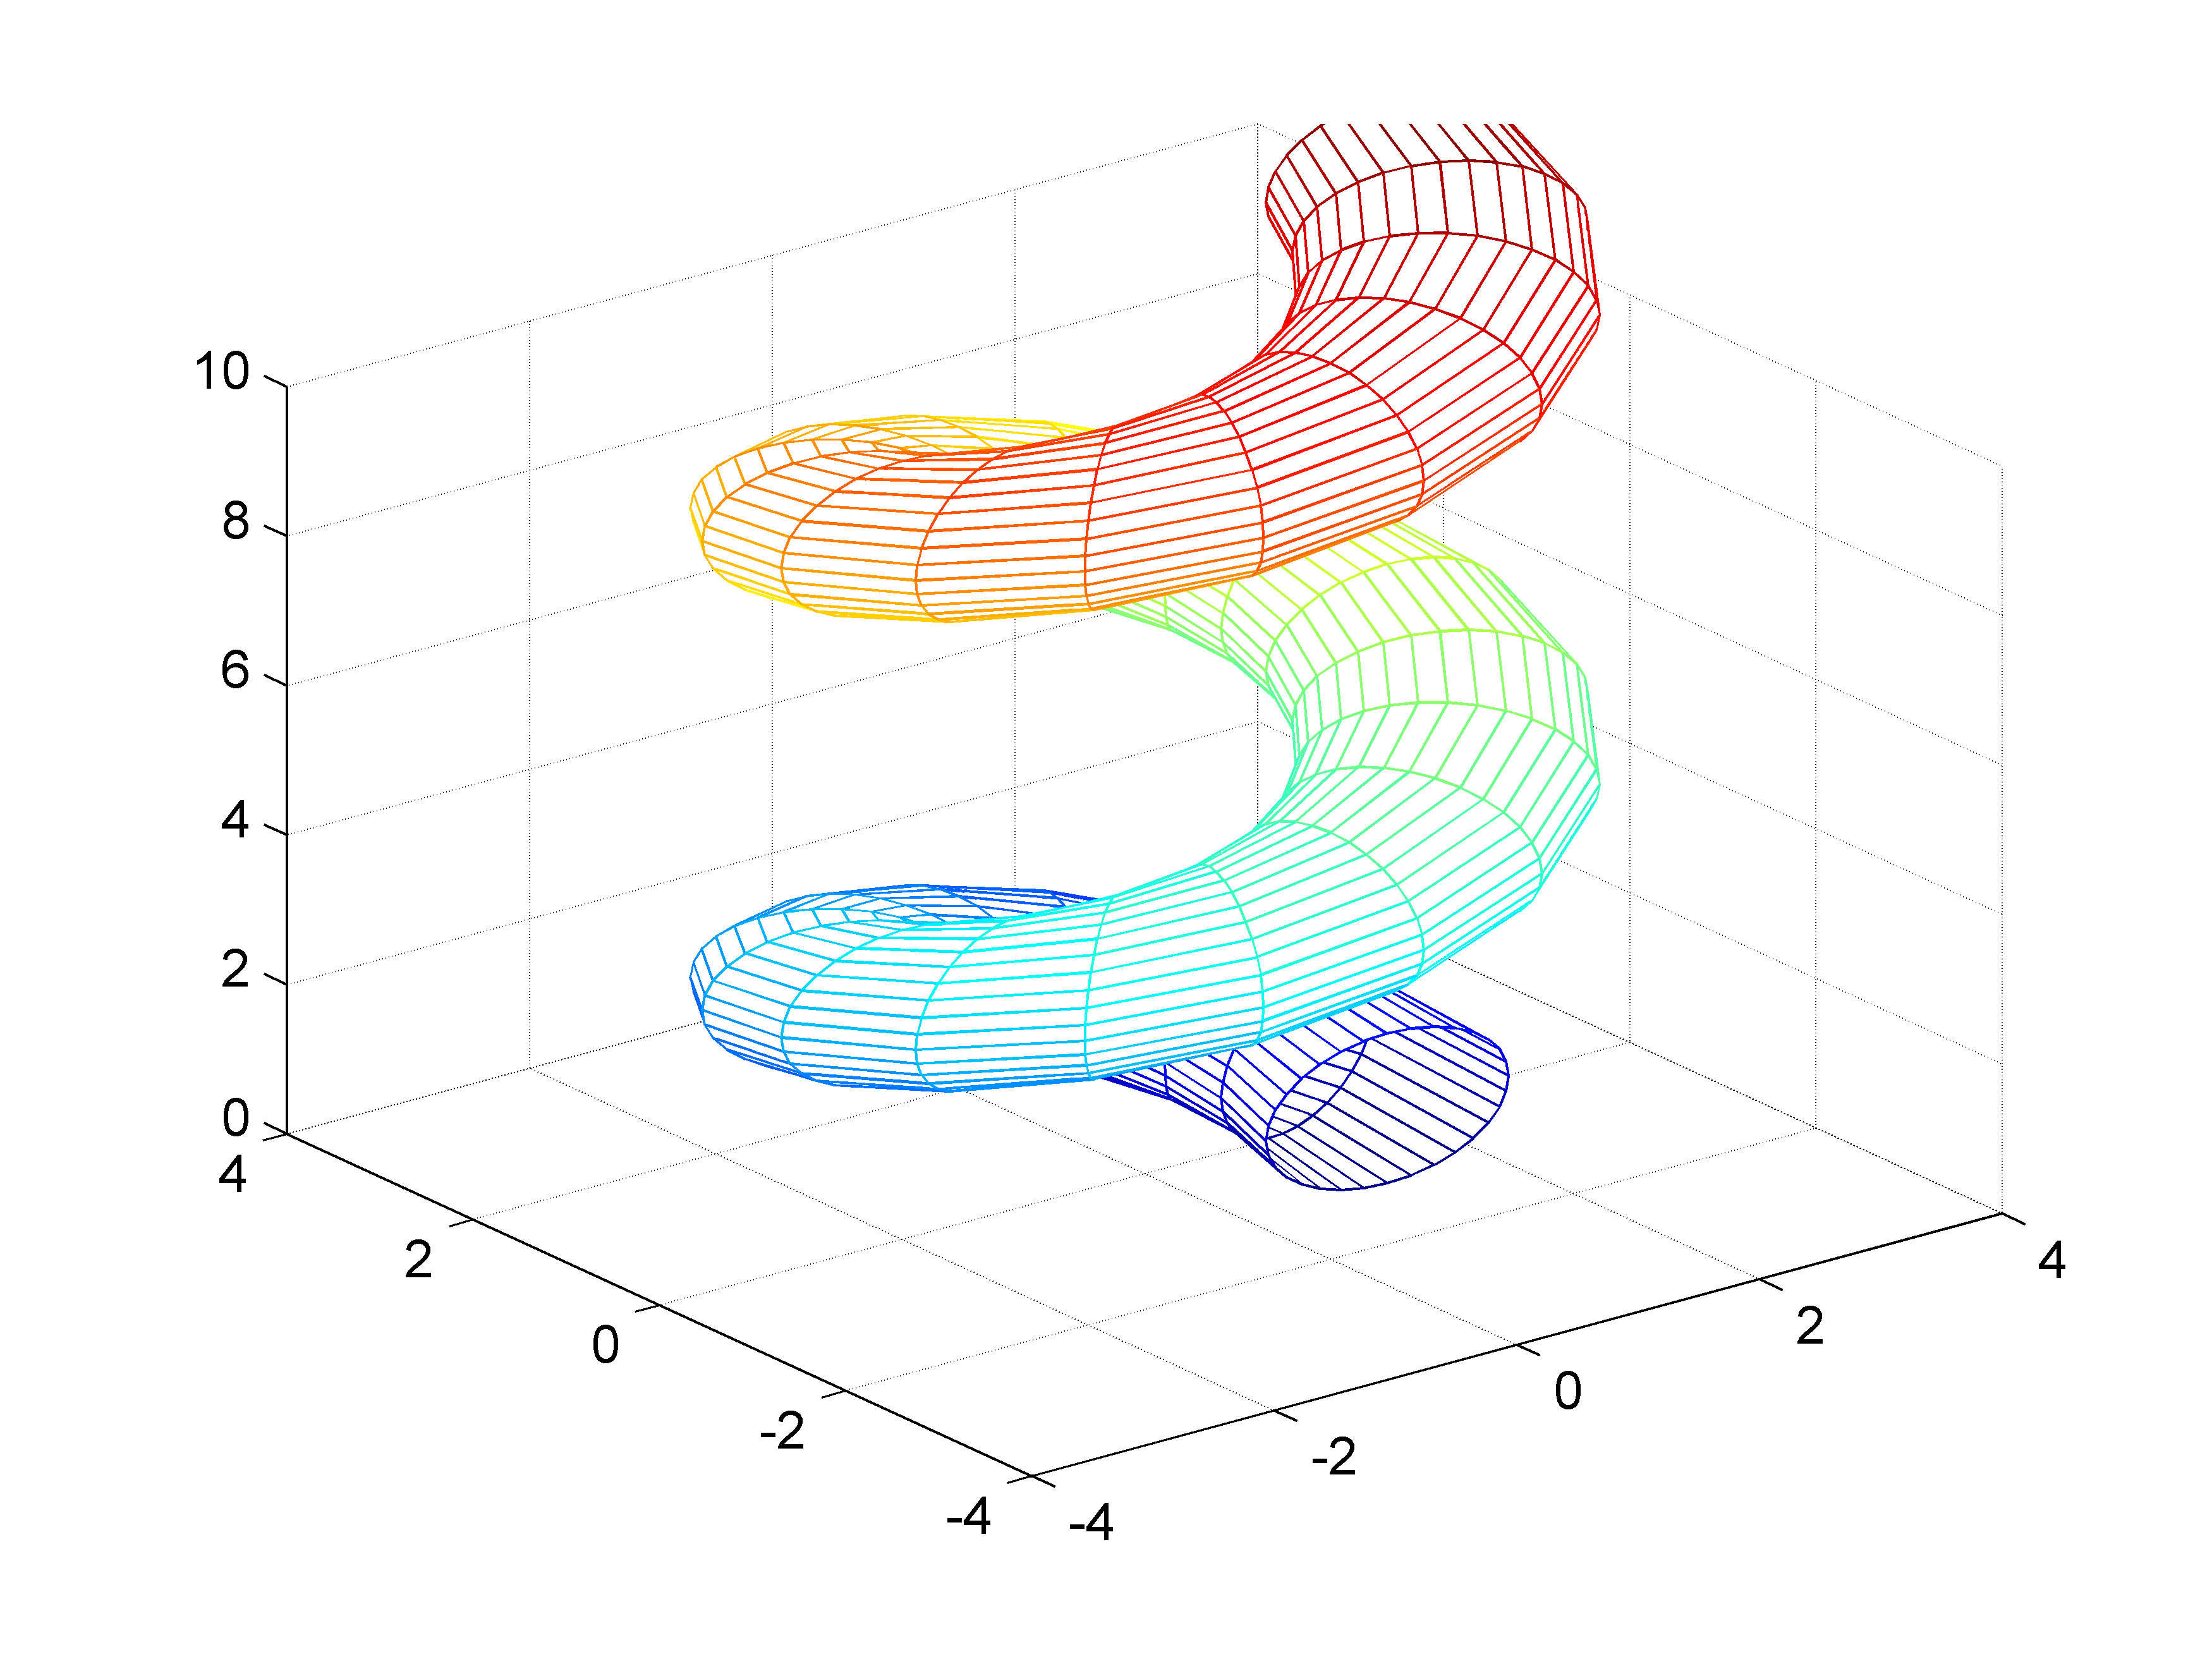
\includegraphics[width=300pt]{./Imagenes/tobogan.png}


\item El unicornio
\begin{lstlisting}[language=Matlab]
>> u=linspace(0,6*pi,60);
>> v=linspace(0,2*pi,60);17
>> [u,v]=meshgrid(u,v);
>> x=2*(1-exp(u/(6*pi))).*cos(u).*cos(v/2).^2;
>> y=2*(-1+exp(u/(6*pi))).*sin(u).*cos(v/2).^2;
>> z=1-exp(u/(3*pi))-sin(v)+exp(u/(6*pi)).*sin(v);
>> mesh(x,y,z)
\end{lstlisting}
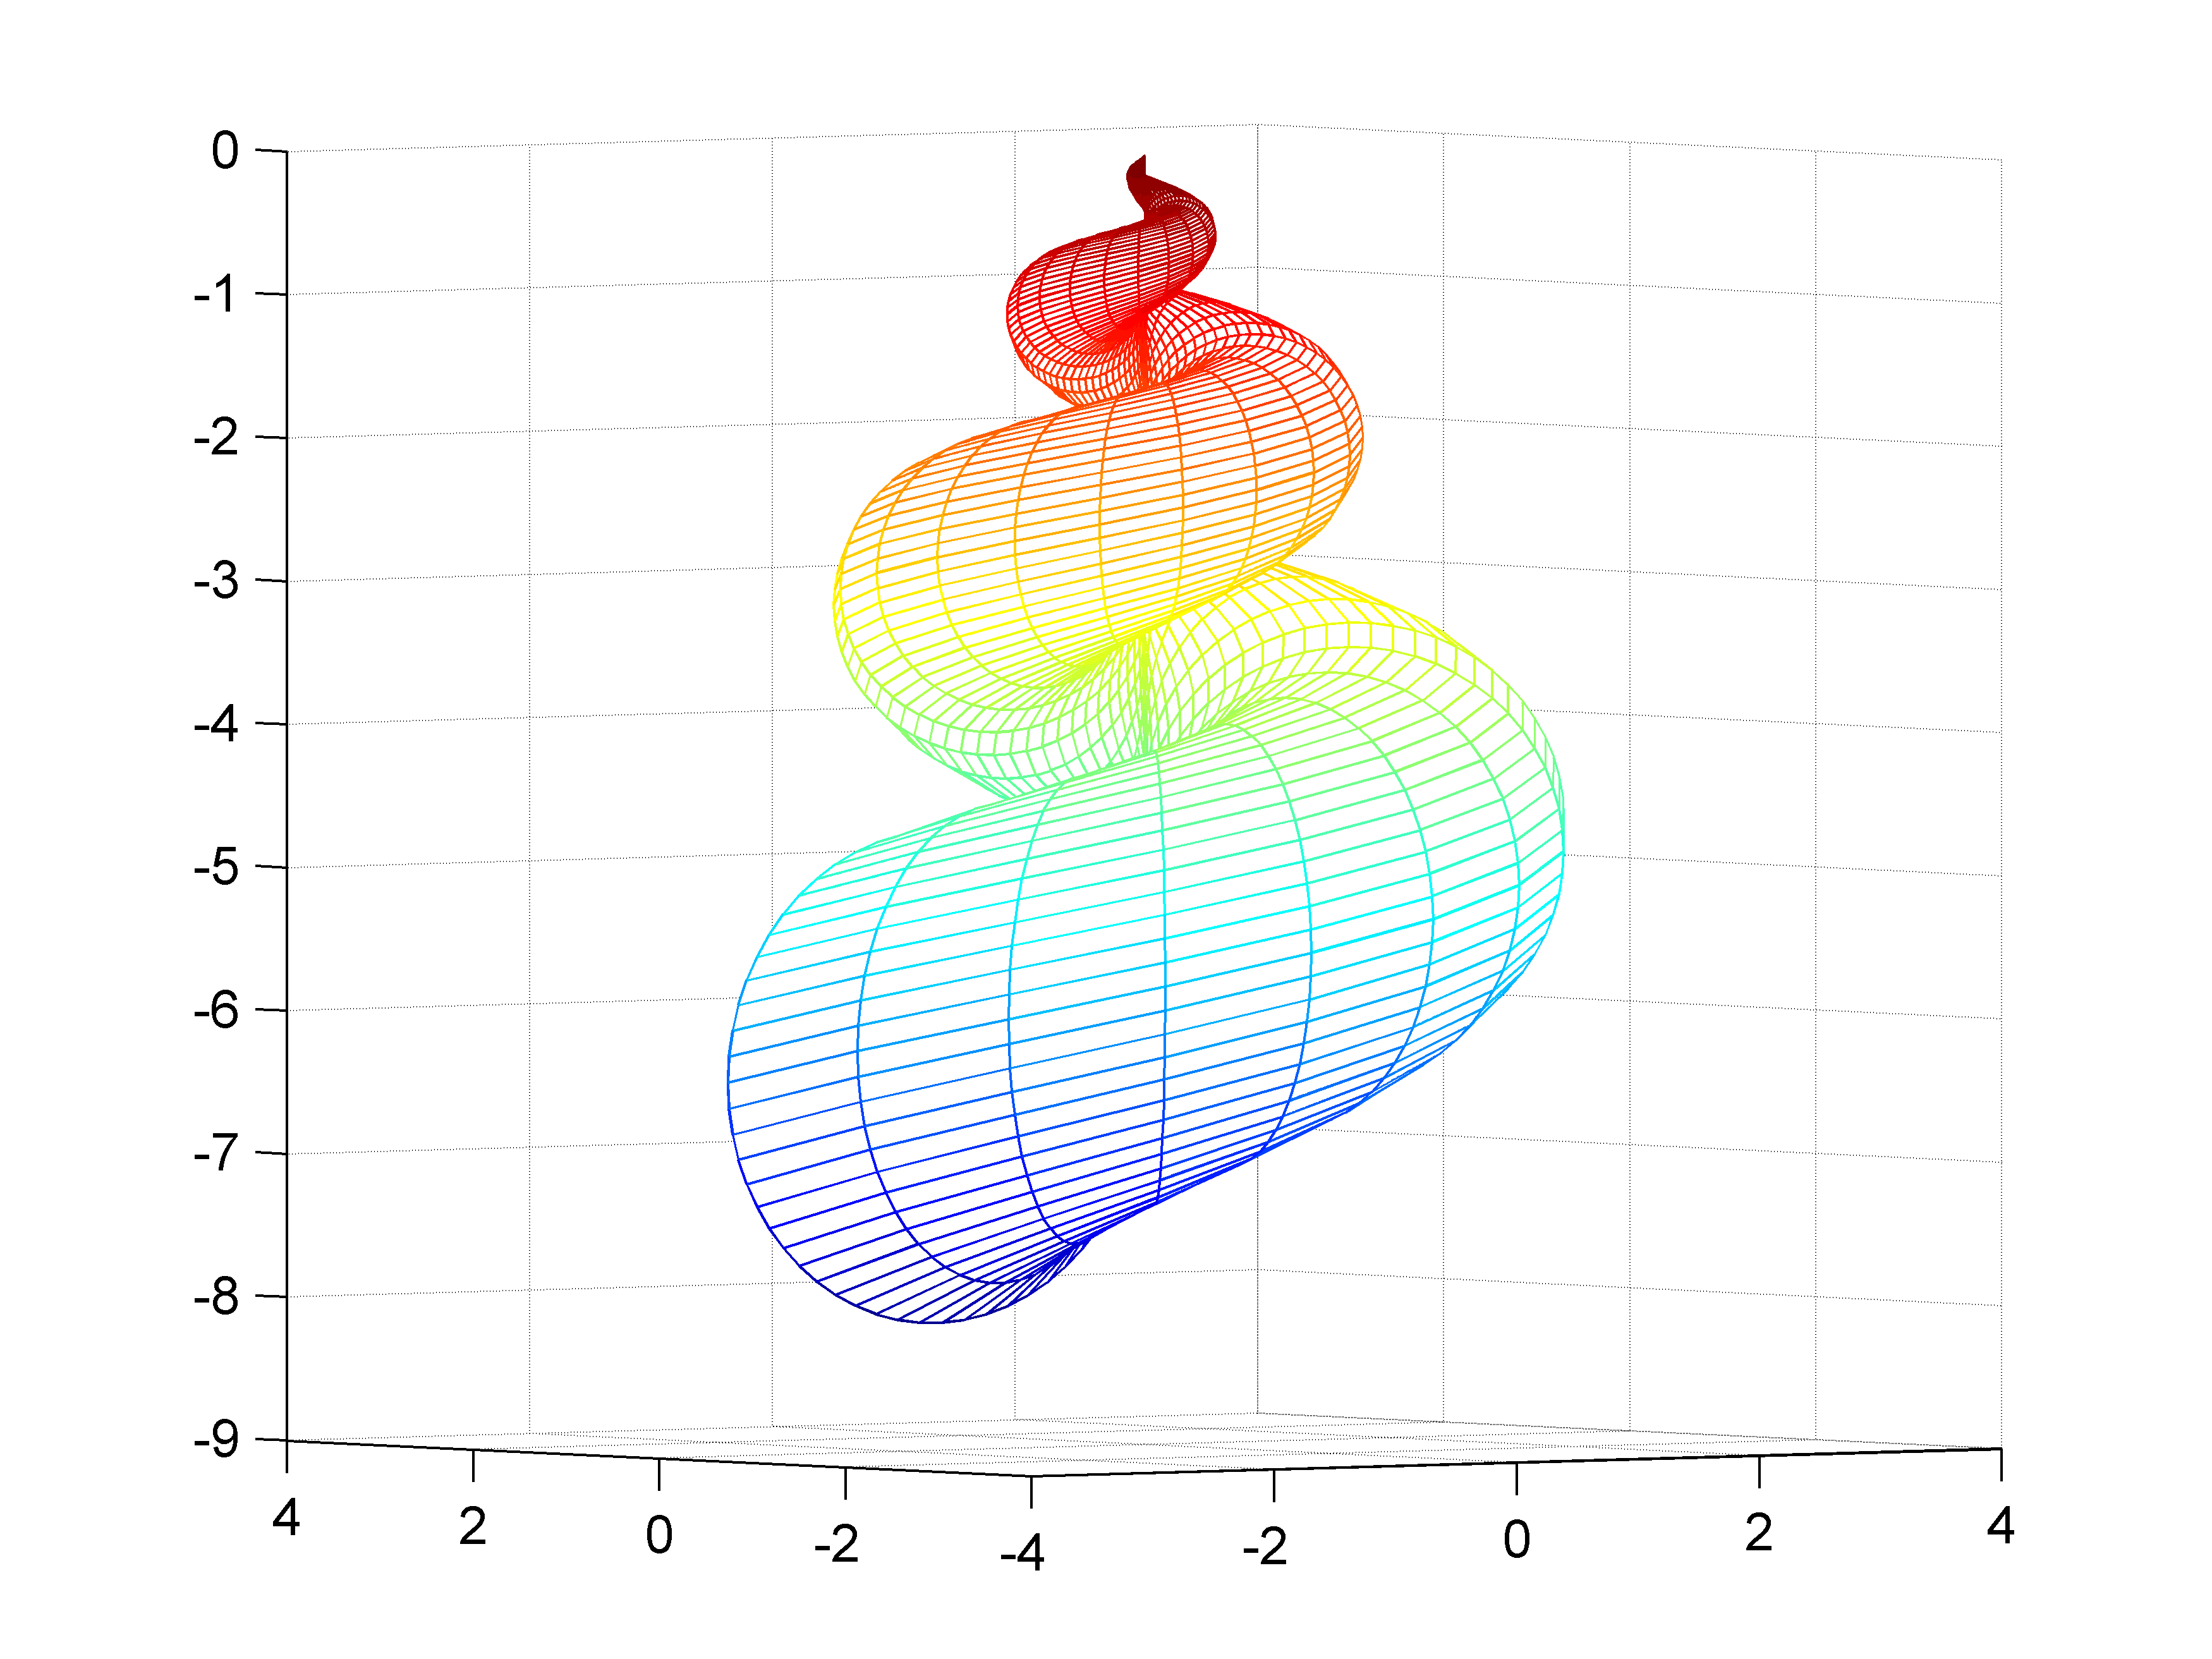
\includegraphics[width=300pt]{./Imagenes/unicornio.png}


\item La Cinta de Möbius. Es una superficie que se puede construir a partir de una tira de papel de forma rectangular ABCD. Torciendo la tira, una sola vez, de manera que se haga 
coincidir el vértice A con el vértice C y el vértice B con el vértice D obteniendo la 
superficie mencionada.

Se genera con la siguiente función vectorial 
$$r(u,v) = [\dfrac{v}{2}*sin(\frac{u}{2}),(1 + \dfrac{v}{2}*cos(\frac{u}{2}))*sin(u),(1 + \dfrac{v}{2}*cos(\frac{u}{2}))*cos(u)]$$ donde $0 \leq u \leq 2\pi ,-1 \lq v \leq 1$

\begin{lstlisting}[language=Matlab]
>> u=linspace(0,2*pi,30);
>> v=linspace(-1,1,15);
>> [u,v]=meshgrid(u,v);
>> z=(1+v/2.*cos(u/2)).*cos(u);
>> y=(1+v/2.*cos(u/2)).*sin(u);
>> x=v/2.*sin(u/2);
>> surf(x,y,z)
\end{lstlisting}
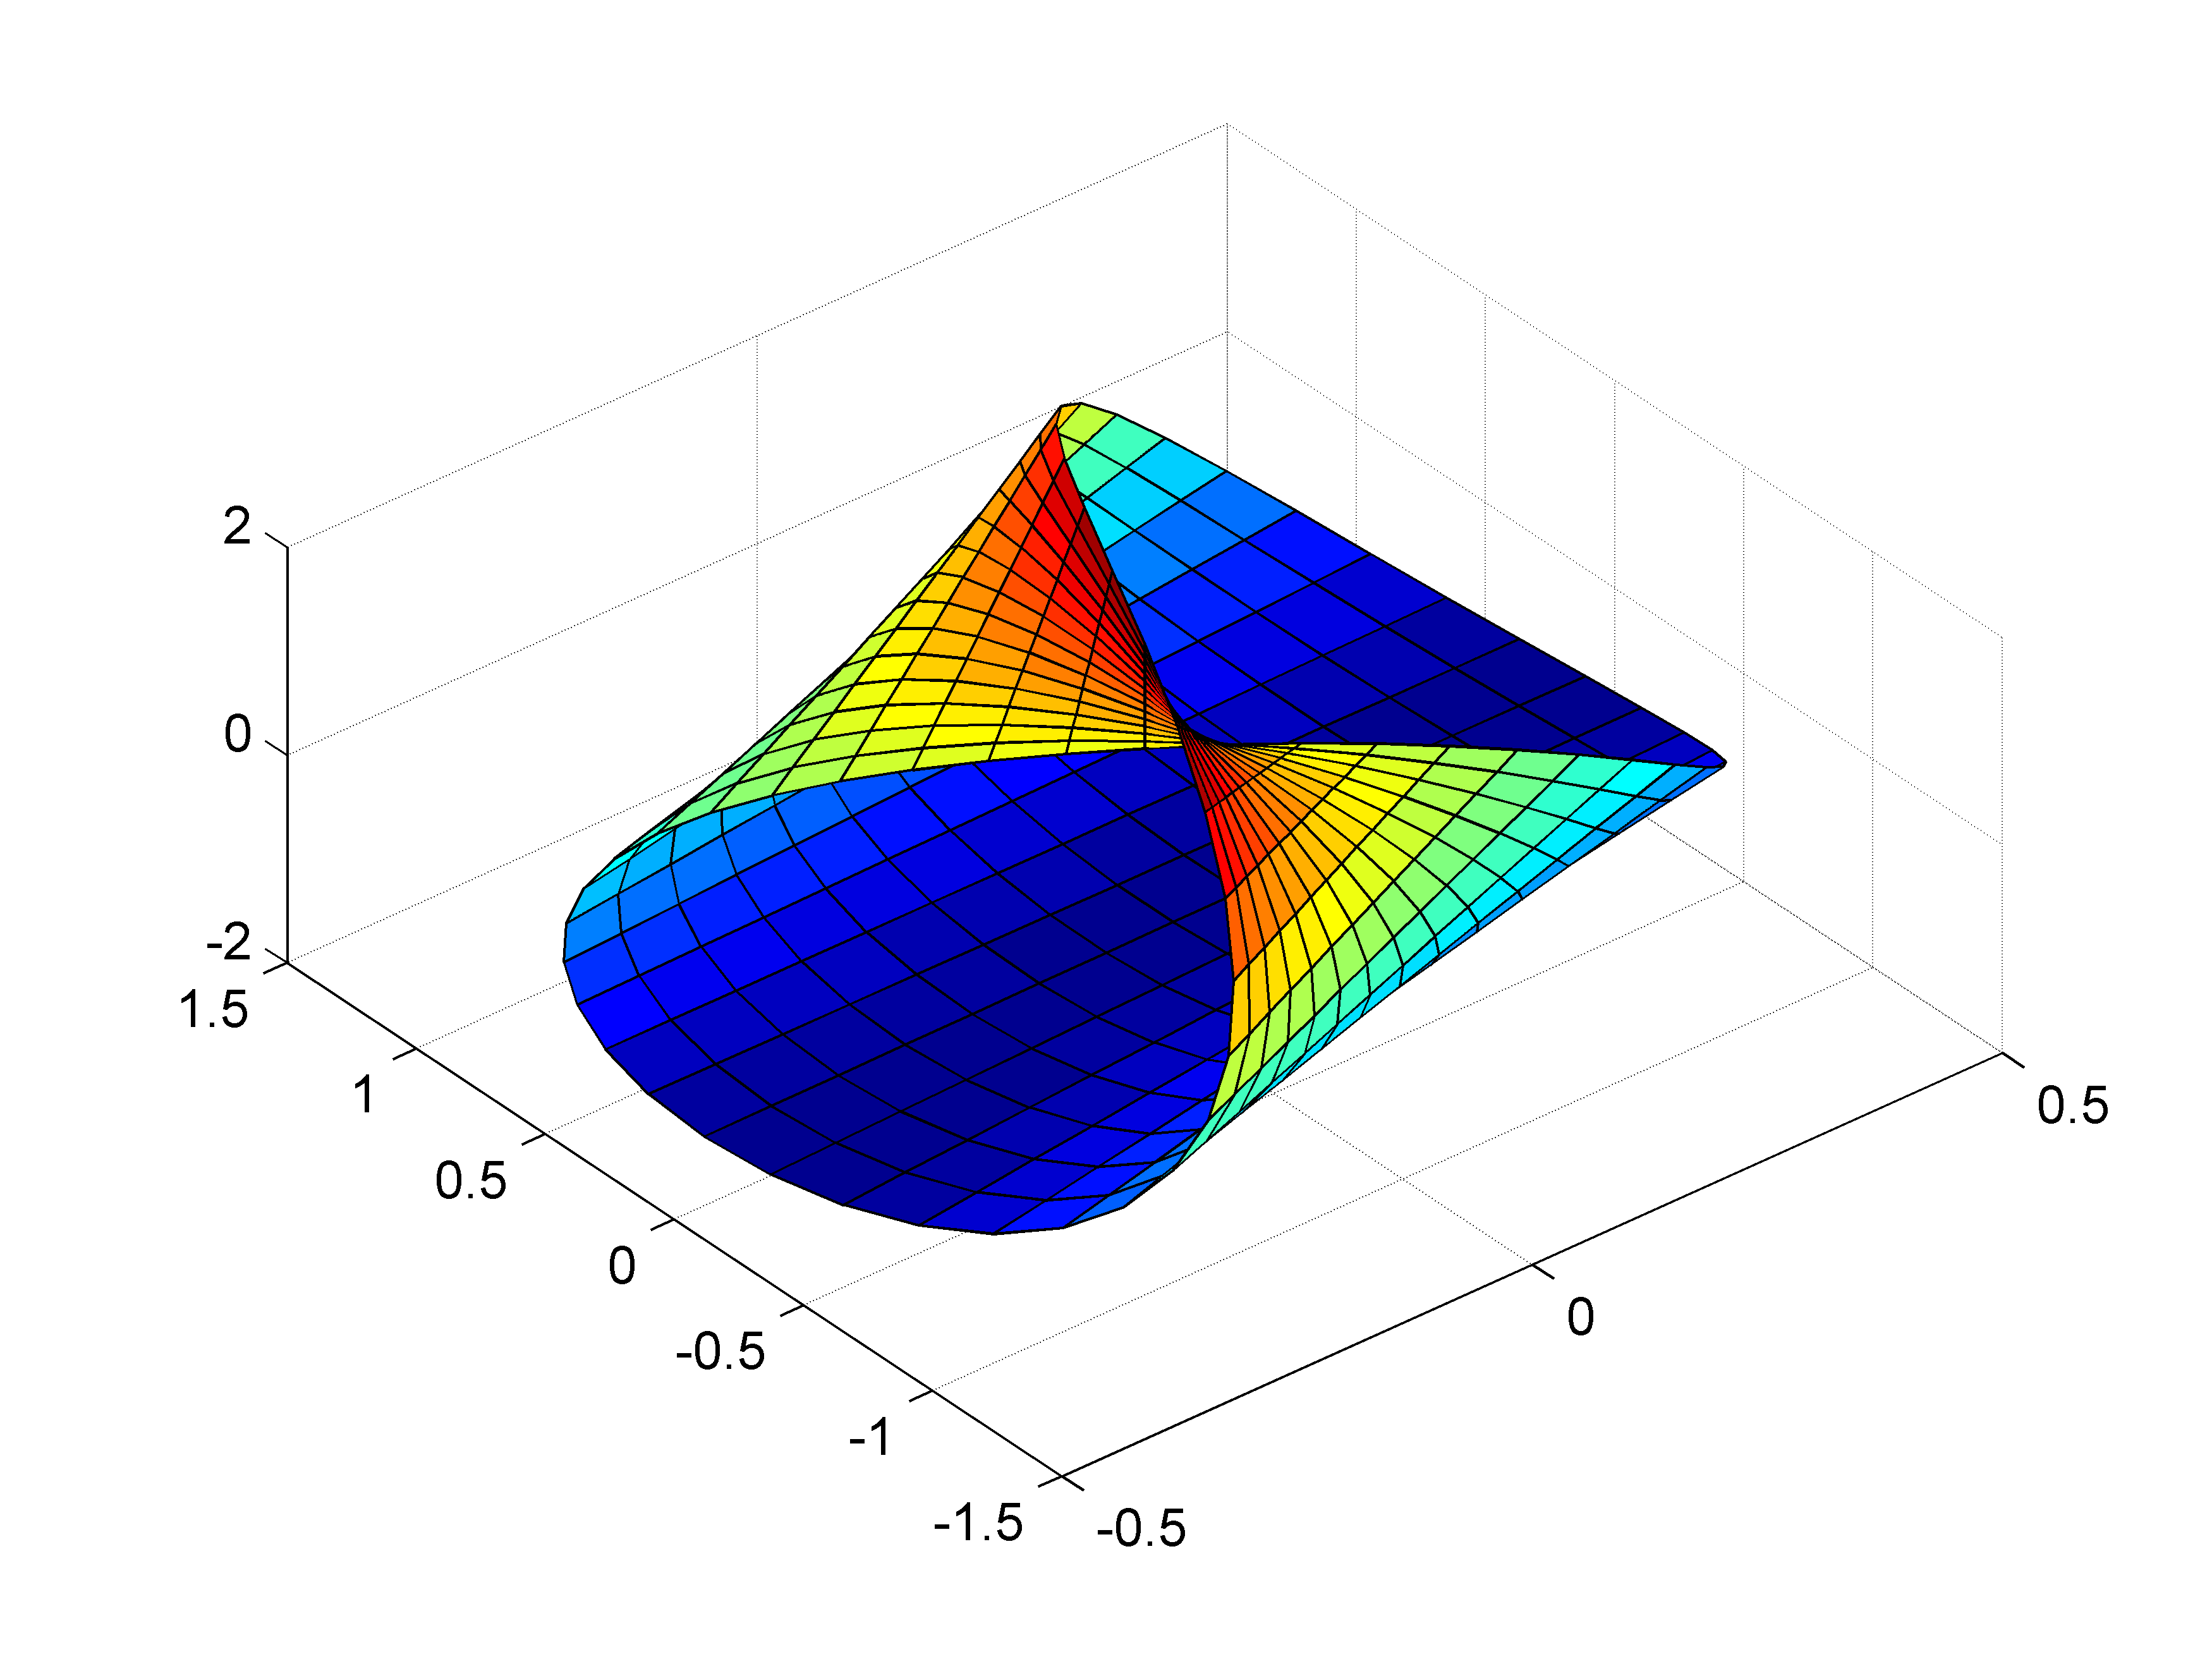
\includegraphics[width=300pt]{./Imagenes/cinta.png}

\end{enumerate}